%% abtex2-modelo-trabalho-academico.tex, v-1.9.2 laurocesar
%% Copyright 2012-2017 by abnTeX2 group at http://abntex2.googlecode.com/ 
%%
%% This work may be distributed and/or modified under the
%% conditions of the LaTeX Project Public License, either version 1.3
%% of this license or (at your option) any later version.
%% The latest version of this license is in
%%   http://www.latex-project.org/lppl.txt
%% and version 1.3 or later is part of all distributions of LaTeX
%% version 2005/12/01 or later.
%%
%% This work has the LPPL maintenance status `maintained'.
%% 
%% The Current Maintainer of this work is Emílio Eiji Kavamura,
%% eek.edu@outlook.com; emilio.kavamura@ufpr.br
%% Further information about abnTeX2 are available on 
%%
%% http://abntex2.googlecode.com/
%%
%% https://code.google.com/p/abntex2/issues/ 
%% Further information about UFPR abnTeX2 are available on 
%%
%% https://github.com/eekBR/ufpr-abntex/
%%
%% This work consists of the files 
% 
%          main.tex   programa principal
%      00-dados.tex   entrada de dados 
%    00-pacotes.tex   pacotes carregados no modelo
% 00-pretextual.tex   processamento dos elementos pre-textuais
%          UFPR.sty   ajusta do modelo canonico às normas  UFPR
%
%    referencias.bib
%
%
%
%------------------------------------------------------------------------
% ------------------------------------------------------------------------
% abnTeX2: Modelo de Trabalho Academico (tese de doutorado, dissertacao de
% mestrado e trabalhos monograficos em geral) em conformidade com 
% ABNT NBR 14724:2011: Informacao e documentacao - Trabalhos academicos -
% Apresentacao
% ------------------------------------------------------------------------
% ------------------------------------------------------------------------

\documentclass[
        % -- opções da classe memoir --
        12pt,                           % tamanho da fonte
        openright,                      % capítulos começam em pág ímpar (insere página vazia caso preciso)
        %twoside,                        % para impressão em verso e anverso. Oposto a oneside
        oneside,
        a4paper,                        % tamanho do papel. 
        % -- opções da classe abntex2 --
        chapter=TITLE,         % títulos de capítulos convertidos em letras maiúsculas
        section=TITLE,         % títulos de seções convertidos em letras maiúsculas
        subsection=Title,      % títulos de subseções convertidos em letras maiúsculas
        %subsubsection=TITLE,  % títulos de subsubseções convertidos em letras maiúsculas
        % -- opções do pacote babel --
        english,                        % idioma adicional para hifenização
        french,                         % idioma adicional para hifenização
        spanish,                        % idioma adicional para hifenização
        portugues,                      % o último idioma é o principal do documento
        %%%%%%%%%%%%
        %eek: colocação da opção para o sumario ter formatação tradicional
        sumario=tradicional             % título no formato tradicional
        ]{abntex2}


\usepackage{UFPR}
\usepackage{subcaption}
\usepackage{physics}
% Pacotes básicos 
% ----------------------------------------------------------
%\usepackage{lmodern}			% Usa a fonte Latin Modern			
\usepackage[T1]{fontenc}		% Selecao de codigos de fonte.
\usepackage[utf8]{inputenc}		% Codificacao do documento (conversão automática dos acentos)
\usepackage{lastpage}			% Usado pela Ficha catalográfica
\usepackage{indentfirst}		% Indenta o primeiro parágrafo de cada seção.
\usepackage{color}		    	% Controle das cores
\usepackage{graphicx}			% Inclusão de gráficos
\usepackage{microtype} 			% para melhorias de justificação
\usepackage{ifthen}		    	% para montar condicionais
\usepackage[brazil]{babel}		% para utilizar termos em portugues
\usepackage[final]{pdfpages}    % para incluir páginas de arquivos pdf
\usepackage{lipsum}				% para geração de dummy text
\usepackage{csquotes}

%\usepackage[style=long]{glossaries}
%\usepackage{abntex2glossaries}

% permite representar o cancelamento de termos em texto ou equacoes
\usepackage{cancel} 		
% cores extendidas
\usepackage{xcolor} 		
% gera diagramas a partir de listas
\usepackage{smartdiagram}   
% Para a figura ficar na posição correta
\usepackage{float} 		    
% supporte para fontes da Text Companion 
\usepackage{textcomp} 		
% uso de longtable
\usepackage{longtable}		
% simbolos matematicos
\usepackage{amsmath}	
% páginas em paisagem
\usepackage{lscape}
% mescla de colunas em tabelas
\usepackage{multicol}
% mescla de linhas em tabelas
\usepackage{multirow}
% criação do indice de quadros
\usepackage{newfloat} 
% configura legenda 
\usepackage{caption}

\usepackage{amsfonts}

% Pacote de física
\usepackage{physics}
%[format=plain]
	%\renewcommand\caption[1]{%
    \captionsetup{font=small}	% tamanho da fonte 10pt
    %,format=hang
 	% \caption{#1}}
	%\captionsetup{width=0.8\textwidth}

% Pacotes de citações BibLaTeX
% ----------------------------------------------------------
\usepackage[style=abnt,backref=true,backend=biber,citecounter=true,backrefstyle=three]{biblatex}
% \usepackage[alf, abnt-emphasize=bf]{abntcite}


\DefineBibliographyStrings{brazil}{%
 backrefpage = {Citado \arabic{citecounter} vez na página},% originally "cited on page"
 backrefpages = {Citado \arabic{citecounter} vezes nas páginas},% originally "cited on pages"
}

% ----------------------------------------------------------

% alterando o aspecto da cor azul
\definecolor{blue}{RGB}{55,10,249}

% ----------------------------------------------------------
\PrepareListOf{quadro}{%
\renewcommand{\cftfigpresnum}{Quadro~}}

\DeclareFloatingEnvironment[
fileext=loq,
listname={\textbf{LISTA DE QUADROS}},
name=Quadro,
%placement=p,
within= none, % numeracao continua
%within=section, % numeracao reinicia em cada seccao
%chapterlistsgaps=off
]{quadro}

\newlistentry{quadro}{loq}{0}


% Customize ‘List of Diagrams’
\PrepareListOf{quadro}{%
\renewcommand{\cftquadropresnum}{\normalsize{QUADRO}~}
\setlength{\cftquadronumwidth}{3.2cm}
%\renewcommand{\cftquadroname}{\quadroname\space} 
\renewcommand*{\cftquadroaftersnum}{\hfill--\hfill}
}

\makeatletter
%% we define a helper macro for adjusting lists of new floats to
%% accept a * behind them for not being shown in the TOC, like
%% the other list printing commands in memoir
\newcommand{\AdjustForMemoir}[1]{%
  \csletcs{kept@listof#1}{listof#1}%
  \csdef{listof#1}{%
    \@ifstar
     {\csappto{newfloat@listof#1@hook}{\append@star}%
      \csuse{kept@listof#1}}%
     {\csuse{kept@listof#1}}%
  }
}
\def\append@star#1{#1*}
\makeatother


\AdjustForMemoir{quadro} % prepare `\listofdirfigures` so it accepts a *

\makeatletter
\let\oldcontentsline\contentsline
\def\contentsline#1#2{%
    \expandafter\ifx\csname l@#1\endcsname\l@section
	\expandafter\@firstoftwo
	\else
	\expandafter\@secondoftwo
	\fi
	{%
		\oldcontentsline{#1}{\MakeTextUppercase{#2}}%
	}{%
	\normalsize %ajusta tamanho da fonte na lista
	\oldcontentsline{#1}{#2}%
}%
}
\makeatother

% Ajusta indentação de Referencias no ToC
% ----------------------------------------------------------
\defbibheading{bay}[\bibname]{%
  \chapter*{#1}%
  \markboth{#1}{#1}%
  \addcontentsline{toc}{chapter}
  {\protect\numberline{}\bibname}
}

\makeatletter
\pretocmd{\chapter}{\addtocontents{toc}{\protect\addvspace{-5\p@}}}{}{}
\pretocmd{\section}{\addtocontents{toc}{\protect\addvspace{2\p@}}}{}{}
\makeatother
%%%%%%%%%%%%%%%%%%%%%%%%%%%%%%%%%%%%%%%%%%%%%%%%%%%%%%%
% Arquivo para entrada de dados para a parte pré textual
%%%%%%%%%%%%%%%%%%%%%%%%%%%%%%%%%%%%%%%%%%%%%%%%%%%%%%%
% 
% Basta digitar as informações indicidas, no formato 
% apresentado.
%
%%%%%%%
% Os dados solicitados são, na ordem:
%
% tipo do trabalho
% componentes do trabalho 
% título do trabalho
% nome do autor
% local 
% data (ano com 4 dígitos)
% orientador(a)
% coorientador(a)(as)(es)
% arquivo com dados bibliográficos
% instituição
% setor
% programa de pós gradução
% curso
% preambulo
% data defesa
% CDU
% errata
% assinaturas - termo de aprovação
% resumos & palavras chave
% agradecimentos
% dedicatoria
% epígrafe


% Informações de dados para CAPA e FOLHA DE ROSTO
%----------------------------------------------------------------------------- 
\tipotrabalho{Dissertação}
%    {Relatório Técnico}
%    {Dissertação}
%    {Tese}
%    {Monografia}

% Marcar Sim para as partes que irão compor o documento pdf
%----------------------------------------------------------------------------- 
 \providecommand{\terCapa}{Sim}
 \providecommand{\terFolhaRosto}{Sim}
 \providecommand{\terTermoAprovacao}{Sim}
 \providecommand{\terDedicatoria}{Nao}
 \providecommand{\terFichaCatalografica}{Nao}
 \providecommand{\terEpigrafe}{Nao}
 \providecommand{\terAgradecimentos}{Nao}
 \providecommand{\terErrata}{Nao}
 \providecommand{\terListaFiguras}{Sim}
 \providecommand{\terListaTabelas}{Sim}
 \providecommand{\terSiglasAbrev}{Sim}
 \providecommand{\terResumos}{Nao}
 \providecommand{\terSumario}{Sim}
 \providecommand{\terAnexo}{Nao}
 \providecommand{\terApendice}{Nao}
 \providecommand{\terIndiceR}{Nao}
%----------------------------------------------------------------------------- 

\titulo{Acurácia da solução numérica em formulações usando malhas não estruturadas}
\autor{Elton Fernando Doehnert}
\local{Curitiba}
\data{2020} %Apenas ano 4 dígitos

% Orientador ou Orientadora
\orientador{Luciano Araki}
%Prof Emílio Eiji Kavamura, MSc}
\orientadora{
Prof\textordfeminine~Grace Kelly, DSc}
% Pode haver apenas uma orientadora ou um orientador
% Se houver os dois prevalece o feminino.

% Em termos de coorientação, podem haver até quatro neste modelo
% Sendo 2 mulhere e 2 homens.
% Coorientador ou Coorientadora
\coorientador{}%Prof Morgan Freeman, DSc}
\coorientadora{Prof\textordfeminine~Audrey Hepburn, DEng}

% Segundo Coorientador ou Segunda Coorientadora
\scoorientador{}
%Prof Jack Nicholson, DEng}
\scoorientadora{}
%Prof\textordfeminine~Ingrid Bergman, DEng}
% ----------------------------------------------------------
\addbibresource{referencias.bib}

% ----------------------------------------------------------
\instituicao{%
Universidade Federal do Paraná}

\def \ImprimirSetor{}%
%Setor de Tecnologia}

\def \ImprimirProgramaPos{}%Programa de Pós Graduação em Engenharia de Construção Civil}

\def \ImprimirCurso{}%
%Curso de Engenharia Civil}

\preambulo{Dissertação apresentada como requisito parcial à obtenção do grau de Mestre em Métodos Numéricos em Engenharia pelo Programa de PósGraduação em Métodos Numéricos em Engenharia, Área de Concentração em Dinâmica dos Fluidos Computacional, dos Setores de Tecnologia e de Ciências Exatas, da Universidade Federal do Paraná.
}


%----------------------------------------------------------------------------- 

\newcommand{\imprimirCurso}{}
%Programa de P\'os Gradua\c{c}\~ao em Engenharia da Constru\c{c}\~ao Civil}

\newcommand{\imprimirDataDefesa}{
09 de Dezembro de 2018}

\newcommand{\imprimircdu}{
02:141:005.7}

% ----------------------------------------------------------
\newcommand{\imprimirerrata}{
Elemento opcional da \cites[4.2.1.2]{NBR14724:2011}. Exemplo:

\vspace{\onelineskip}

FERRIGNO, C. R. A. \textbf{Tratamento de neoplasias ósseas apendiculares com
reimplantação de enxerto ósseo autólogo autoclavado associado ao plasma
rico em plaquetas}: estudo crítico na cirurgia de preservação de membro em
cães. 2011. 128 f. Tese (Livre-Docência) - Faculdade de Medicina Veterinária e
Zootecnia, Universidade de São Paulo, São Paulo, 2011.

\begin{table}[htb]
\center
\footnotesize
\begin{tabular}{|p{1.4cm}|p{1cm}|p{3cm}|p{3cm}|}
  \hline
   \textbf{Folha} & \textbf{Linha}  & \textbf{Onde se lê}  & \textbf{Leia-se}  \\
    \hline
    1 & 10 & auto-conclavo & autoconclavo\\
   \hline
\end{tabular}
\end{table}}

% Comandos de dados - Data da apresentação
\providecommand{\imprimirdataapresentacaoRotulo}{}
\providecommand{\imprimirdataapresentacao}{}
\newcommand{\dataapresentacao}[2][\dataapresentacaoname]{\renewcommand{\dataapresentacao}{#2}}

% Comandos de dados - Nome do Curso
\providecommand{\imprimirnomedocursoRotulo}{}
\providecommand{\imprimirnomedocurso}{}
\newcommand{\nomedocurso}[2][\nomedocursoname]
  {\renewcommand{\imprimirnomedocursoRotulo}{#1}
\renewcommand{\imprimirnomedocurso}{#2}}


% ----------------------------------------------------------
\newcommand{\AssinaAprovacao}{

\assinatura{%\textbf
   {Professora} \\ UFPR}
   \assinatura{%\textbf
   {Professora} \\ ENSEADE}
   \assinatura{%\textbf
   {Professora} \\ TIT}
   %\assinatura{%\textbf{Professor} \\ Convidado 4}
      
   \begin{center}
    \vspace*{0.5cm}
    %{\large\imprimirlocal}
    %\par
    %{\large\imprimirdata}
    \imprimirlocal, \imprimirDataDefesa.
    \vspace*{1cm}
  \end{center}
  }
  
% ----------------------------------------------------------
%\newcommand{\Errata}{%\color{blue}
%Elemento opcional da \textcite[4.2.1.2]{NBR14724:2011}. Exemplo:
%}

% ----------------------------------------------------------
\newcommand{\EpigrafeTexto}{%\color{blue}
\textit{``Não vos amoldeis às estruturas deste mundo, \\
		mas transformai-vos pela renovação da mente, \\
		a fim de distinguir qual é a vontade de Deus: \\
		o que é bom, o que Lhe é agradável, o que é perfeito.\\
		(Bíblia Sagrada, Romanos 12, 2)}
}

% ----------------------------------------------------------
\newcommand{\ResumoTexto}{%\color{blue}
Segundo a \textcite[3.1-3.2]{abntex2modelo}, o resumo deve ressaltar o  objetivo, o método, os resultados e as conclusões do documento. A ordem e a extensão destes itens dependem do tipo de resumo (informativo ou indicativo) e do tratamento que cada item recebe no documento original. O resumo deve ser precedido da referência do documento, com exceção do resumo inserido no próprio documento. (\ldots) As palavras-chave devem figurar logo abaixo do  resumo, antecedidas da expressão Palavras-chave:, separadas entre si por ponto e finalizadas também por ponto.
}

\newcommand{\PalavraschaveTexto}{%\color{blue}
latex. abntex. editoração de texto.}

% ----------------------------------------------------------
\newcommand{\AbstractTexto}{%\color{blue}
This is the english abstract.
}
% ---
\newcommand{\KeywordsTexto}{%\color{blue}
latex. abntex. text editoration.
}

% ----------------------------------------------------------
\newcommand{\Resume}
{%\color{blue}
%Il s'agit d'un résumé en français.
} 
% ---
\newcommand{\Motscles}
{%\color{blue}
 %latex. abntex. publication de textes.
}

% ----------------------------------------------------------
\newcommand{\Resumen}
{%\color{blue}
%Este es el resumen en español.
}
% ---
\newcommand{\Palabrasclave}
{%\color{blue}
%latex. abntex. publicación de textos.
}

% ----------------------------------------------------------
\newcommand{\AgradecimentosTexto}{%\color{blue}
Os agradecimentos principais são direcionados à Gerald Weber, Miguel Frasson, Leslie H. Watter, Bruno Parente Lima, Flávio de  Vasconcellos Corrêa, Otavio Real Salvador, Renato Machnievscz\footnote{Os nomes dos integrantes do primeiro
projeto abn\TeX\ foram extraídos de \url{http://codigolivre.org.br/projects/abntex/}} e todos aqueles que contribuíram para que a produção de trabalhos acadêmicos conforme as normas ABNT com \LaTeX\ fosse possível.

Agradecimentos especiais são direcionados ao Centro de Pesquisa em Arquitetura da Informação\footnote{\url{http://www.cpai.unb.br/}} da Universidade de Brasília (CPAI), ao grupo de usuários
\emph{latex-br}\footnote{\url{http://groups.google.com/group/latex-br}} e aos novos voluntários do grupo \emph{\abnTeX}\footnote{\url{http://groups.google.com/group/abntex2} e
\url{http://abntex2.googlecode.com/}}~que contribuíram e que ainda
contribuirão para a evolução do \abnTeX.

Os agradecimentos principais são direcionados à Gerald Weber, Miguel Frasson, Leslie H. Watter, Bruno Parente Lima, Flávio de Vasconcellos Corrêa, Otavio Real Salvador, Renato Machnievscz\footnote{Os nomes dos integrantes do primeiro
projeto abn\TeX\ foram extraídos de \url{http://codigolivre.org.br/projects/abntex/}} e todos aqueles que contribuíram para que a produção de trabalhos acadêmicos conforme as normas ABNT com \LaTeX\ fosse possível.
}

% ----------------------------------------------------------
\newcommand{\DedicatoriaTexto}{%\color{blue}
\textit{ Este trabalho é dedicado às crianças adultas que,\\
   quando pequenas, sonharam em se tornar cientistas.}
	}



% compila o indice
% ----------------------------------------------------------

\makeindex
% ----------------------------------------------------------
% Início do documento
% ----------------------------------------------------------
\begin{document}
% ----------------------------------------------------------
% Adequando o uppercase titulo dos elementos nas suas respectivas legendas
% Definicoes que n\~ao funcionaram quando colocados no arquivo de estilos ou de pacotes

\renewcommand{\bibname}{{REFER\^ENCIAS}}
\renewcommand{\tablename}{TABELA }
\renewcommand{\figurename}{FIGURA }
\renewcommand{\figureautorefname}{FIGURA}
\renewcommand{\tableautorefname}{TABELA}

% ELEMENTOS PRÉ-TEXTUAIS
% ----------------------------------------------------------
% Capa
% ----------------------------------------------------------
 \ifthenelse{\equal{\terCapa}{Sim}}{
\imprimircapa}{}

% Folha de rosto
% ----------------------------------------------------------
\imprimirfolhaderosto*

% Inserir a ficha bibliografica
% ----------------------------------------------------------
 \ifthenelse{\equal{\terFichaCatalografica}{Sim}}
 {\insereFichaCatalografica{}\cleardoublepage}
 {}

% Inserir errata
% ----------------------------------------------------------
 \ifthenelse{\equal{\terErrata}{Sim}}
 {\begin{errata}%\color{blue}
   \imprimirerrata
  \end{errata}}
 {}

% Inserir folha de aprovação
% ----------------------------------------------------------
\ifthenelse{\equal{\terTermoAprovacao}{Sim}}{
\insereAprovacao}{}

% Dedicatória
% ----------------------------------------------------------
\ifthenelse{\equal{\terDedicatoria}{Sim}}{
\begin{dedicatoria}
   \vspace*{\fill}
   \centering
   \noindent
   \DedicatoriaTexto
   \vspace*{\fill}
\end{dedicatoria}
}{}

% Agradecimentos
% ----------------------------------------------------------

 \ifthenelse{\equal{\terAgradecimentos}{Sim}}
 {\begin{agradecimentos}
    \AgradecimentosTexto
  \end{agradecimentos}
  }{}
% Epígrafe
% ----------------------------------------------------------

\ifthenelse{\equal{\terEpigrafe}{Sim}}{
\begin{epigrafe}
    \vspace*{\fill}
	\begin{flushright}
        \EpigrafeTexto
	\end{flushright}
\end{epigrafe}
}{}

% RESUMOS
% ----------------------------------------------------------
% resumo em português
%\setlength{\absparsep}{18pt} % ajusta o espaçamento dos parágrafos do resumo
 \ifthenelse{\equal{\terResumos}{Sim}}{
\begin{resumo}
    \ResumoTexto
    
    %\vspace{\onelineskip}
    \noindent 
    \textbf{Palavras-chaves}: \PalavraschaveTexto
\end{resumo}

%% resumo em inglês
\begin{resumo}[ABSTRACT]
 \begin{otherlanguage*}{english}
   \AbstractTexto
   
   %\vspace{\onelineskip}
   \noindent 
   \textbf{Key-words}: \KeywordsTexto
 \end{otherlanguage*}
\end{resumo}


% resumo em francês 
\ifthenelse{\equal{\Resume}{}}
{}
{
 \begin{resumo}[RESUME]%Résumé
  \begin{otherlanguage*}{french}
     \Resume
     
     %\vspace{\onelineskip}
     \noindent      
     \textbf{Mots clés}: \Motscles
  \end{otherlanguage*}
 \end{resumo}
} 

% resumo em espanhol
\ifthenelse{\equal{\Resume}{}}{}
{ \begin{resumo}[RESUMEN]
  \begin{otherlanguage*}{spanish}
    \Resumen 
   
   %\vspace{\onelineskip}
   \noindent    
    \textbf{Palabras clave}: \Palabrasclave
  \end{otherlanguage*}
 \end{resumo}
}
}{}

% inserir lista de ilustrações
% ----------------------------------------------------------
\ifthenelse{\equal{\terListaFiguras}{Sim}}{
%\pdfbookmark[0]{\listfigurename}{lof}
\listoffigures*
\cleardoublepage
}{}


% inserir lista de tabelas
% ----------------------------------------------------------
\ifthenelse{\equal{\terListaTabelas}{Sim}}{
%\pdfbookmark[0]{\listtablename}{lot}
\listoftables*
\cleardoublepage
}{}


% inserir lista de abreviaturas e siglas 
% inserir lista de símbolos
% ----------------------------------------------------------

 \ifthenelse{\equal{\terSiglasAbrev}{Sim}}{
    \imprimirlistadesiglas
    \cleardoublepage
    \imprimirlistadesimbolos
    \cleardoublepage
 }{}

% inserir o sumario
% ----------------------------------------------------------
\ifthenelse{\equal{\terSumario}{Sim}}{
%\pdfbookmark[0]{\contentsname}{toc}
\tableofcontents*
%\cleardoublepage
}{}
 

 
 


% ----------------------------------------------------------
% ELEMENTOS TEXTUAIS
% ----------------------------------------------------------
\textual % \pagestyle{textualUFPR}

\pagestyle{simple}
% sugerido por Youssef Cherem 20170316
% https://mail.google.com/mail/u/0/?tab=wm#inbox/15ad3fe6f4e5ff1f

% Introdução (exemplo de capítulo sem numeração, mas presente no Sumário)
% ----------------------------------------------------------
\chapter[INTRODUÇÃO]{INTRODUÇÃO}
%---------------------------------------------------------------------------------------

A simulação numérica de problemas na engenharia possui uma grande importância tanto para o meio acadêmico quanto para a indústria favorecendo o desenvolvimento de novas tecnologias. Dado esse interesse, novas técnicas para aumentar a acurácia das simulações numéricas são de grande importância.

Esse trabalho verifica o erro de discretização que ocorre nas soluções do FVM usando-se uma malha não estruturada triangular comparando a solução com a analítica e suavizando a malha com vários algoritmos diferentes.
\criarsigla{FVM}{Método dos Volumes Finitos}

Muitos problemas de engenharia estão relacionados a geometrias complexas, em que o uso de um sistema de coordenadas cartesianas, cilíndricas ou esféricas não se mostra prático ou adequado. No cálculo numérico do fluxo sobre um semi cilindro, conforme a figura \ref{fig:semicilindro} temos que a fronteira da figura não coincide com as linhas coordenadas da malha estruturada, de modo que essa malha não é adequada para esse problema. \cite{Versteeg2007}

\begin{figure}[]
\centering
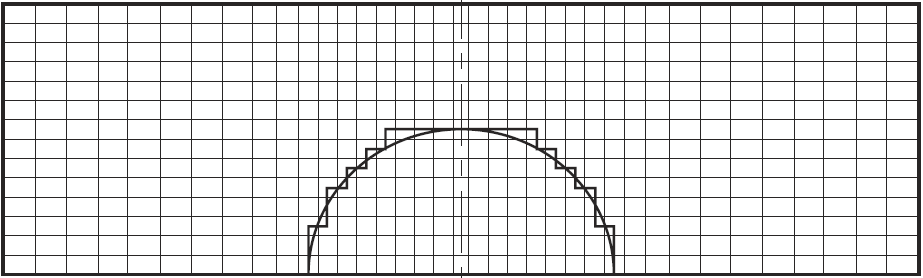
\includegraphics[width=.6\linewidth]{fig/semicilindro.png}
 \caption{Grade cartesiana para prever o fluxo em um semi cilindro}
   \label{fig:semicilindro}
\end{figure}

Malhas cartesianas são exemplos de um método estruturado. Como características de uma malha estruturada, tem-se:

\begin{itemize}
    \item os pontos nodais são posicionados nas interseções das linhas coordenadas.
    \item os pontos nodais interiores (que não estão posicionados nos contornos) possuem um número fixo de pontos nodais vizinhos.
    \item os pontos nodais podem ser mapeados dentro de uma matriz, sua localização na malha e na matriz é fornecida por índices (comumente i,j em problemas 2d e i,j,k em problemas 3d).
\end{itemize}

Os métodos em CFD para geometrias complexas podem ser classificados em malhas não-ortogonais (malhas curvilíneas) estruturadas e em malhas não-estruturadas.

Malhas não-ortogonais estruturadas (ou malhas coincidentes com o corpo / com a fronteira do domínio) são baseadas no mapeamento do "domínio de escoamento" sobre o "domínio computacional" com um formato simples, nota-se contudo, que encontrar um mapeamento viável pode se tornar complicado para geometrias complexas. Neste caso, pode-se recorrer à subdivisão do domínio em diferentes subregiões ou blocos, cada qual apresentando uma malha em separado que deverá ser unida corretamente aos seus vizinhos. Tem-se neste caso as malhas estruturadas por blocos. sdf.

Uma generalização da técnica de malhas estruturadas por blocos é o caso de malhas não-estruturadas, para as quais cada bloco é formado por um único elemento (ou célula). Malhas não-estruturadas garantem uma flexibilidade geométrica ilimitada e são empregadas para escoamentos em geometrias complexas, sendo atualmente a mais empregada técnica em CFD industrial.

Nessas malhas não-estruturadas deve-se, de alguma forma, guardar todos os vizinhos de cada vértice ou elementos. \cite{Shewchuk1992}

Malhas estruturadas possuem como vantagens a obtenção de matrizes diagonais (devido à ordenação), solvers mais fáceis de serem desenvolvidos e mais eficientes e suas equações governantes são descritas de modo mais simples. Já as sua desvantagen é a adaptabilidade para geometrias mais complexas.

No caso de uma malha estruturada mas não-ortogonal, tem-se como vantagens uma maior adaptabilidade para geometrias mais complexas, também se obtém matrizes diagonais com solvers disponíveis e eficientes. Como desvantagens se tem a obtenção de equações governantes de forma mais complexa, maior tempo de geração (devido ao mapeamento que deve ser realizado) e em alguns casos, esse mapeamento é impossível devido a complexidades geométricas.

No caso de uma malha não-estruturada, tem-se como vantagens uma maior versatilidade e adaptabilidade para qualquer complexidade geométrica e uma facilidade de refino local de malha, para pontos de maior interesse (como regiões de recirculação, camadas-limite entre outras). As desvantagens são uma maior complexidade na discretização e a obtenção de matrizes não-diagonais, que devem ser resolvidas usando-se solvers mair gerais e, portanto, menos eficientes.

\section{Acurácia Numérica}
A acurácia numérica na área de dinâmica de fluídos computacional vem tornando-se muito importante na engenharia \cite{doi:10.1080/10407791003685155}. O método mais usado para resolver problemas de fluxo de fluidos é o método dos volumes finitos (FVM), que será discutido no capítulo 2.

O erro de discretização é uma classe de erros muito importante no FVM, que é o método usado nesse trabalho. Existem vários trabalhos cujo objetivo é estimar esse erro de discretização \cite{Muzaferija2014} \cite{Jasak1996} Existem várias maneiras de se estimar esse erro de discretização, esse erro pode ser usado para motivar o refinamento da malha de modo a se controlar o valor desse erro.

Existem análises de vários esquemas de discretização que incluem a influência da qualidade da malha na solução devido a vários parâmetros dessa malha.

Esse erro de discretização é também influenciado pelo tipo de células da malha. \cite{doi:10.1080/10407791003685155}

Esse erro afeta os termos de convecção e difusão para diferentes formatos de volumes de controle, nesse trabalho será considerado apenas células triangulares pois são o tipo mais usado por poderem ser geradas com uma triangularização de Delaunay.

O capítulo 2 apresenta o método dos volumes finitos (FVM) e a dedução para o erro de discretização do termo de convecção e difusão.

De modo a se escrever as equações em um novo sistema de coordenadas é apresentado a teoria necessária para tal conversão começando no capítulo de Transformação de Coordenadas e depois, com a malha gerada, no capítulo Difusão de calor 2D em regime permanente.

A geração de malhas não estruturadas é mostrada no capítulo \ref{MALHAS NAO ESTRUTURADAS}.

\section{OBJETIVOS}

Comparar a acurácia da solução numérica em relação a solução analítica para um problema de transmissão de calor 2D em uma malha em formato 'L' sendo essa malha suavizada usando-se diferentes técnicas, dessa forma comparando-se os métodos de suavização com relação a acurácia da solução analítica e também com relação a um parâmetro de qualidade das malhas que será discutido posteriormente.
Também desenvolver um método de suavização de malhas baseado no algoritmo genético.

\section{IMPORTÂNCIA DO TRABALHO}

Raramente um algoritmo de geração de malhas irá ser capaz de definir uma malha que seja ideal sem alguma forma de pós-processamento para melhorar a qualidade geral dessa malha. \cite{Salama} Dessa forma existe a questão de definir qual método de suavização aplicar na malha gerada levando-se em conta também o custo computacional de modo a se obter o método com o melhor custo-benefício para a simulação computacional em questão. Dessa forma, a determinação de tal método se mostra uma tarefa de grande importância em malhas de grande escala.

\section{ORGANIZAÇÃO DO TRABALHO}

Este trabalho está dividido em 10 capítulos, incluindo-se esta introdução.
O capítulo 2 traz uma revisão da literatura sobre o método dos volumes finitos(FVM), usado na resolução do problema de transmissão de calor 2D, mostra-se as suas vantagens e motivações de uso e a dedução do método.
O capítulo 3 apresenta a teoria para a transformação de coordenadas do domínio físico $(x,y)$ para o domínio computacional $(\xi,\eta)$.
O capítulo 4 define as malhas não estruturadas, a motivação para o seu uso e a discretização usando-se o FVM. Também é mostrado a geração de malhas triangulares, foco do trabalho e métodos de triangulação.
O capítulo 5 é dedicado aos métodos de suavização de malhas não estruturadas com foco em malhas triangulares.
No capítulo 6 é mostrado a dedução para a equação discretizada da difusão de calor 2D em regime permanente.
No capítulo 7 é apresentado a teoria de algoritmos genéticos, usada no método desenvolvido para a suavização da malha.
O capítulo 8 possui o desenvolvimento do projeto.
O capítulo 9 apresenta uma análise dos resultados gerados.
O trabalho finaliza com as conclusões da pesquisa no capítulo 10.

% \cite{ISO5122:1979}
% \textcite{ISO5122:1979}

% \begin{itemize}
%  \item para inserir uma sigla: 
%     \verb|\criarsigla|\{ABNT\}{Associa\c{c}\~ao Brasileira de Normas T\'ecnicas}:

% \criarsigla{ABNT}{teste}

% \item para inserir s\'imbolo: 
%     \verb|\criarsimbolo{$ \Gamma $}{Letra grega Gama}|
  
$ \Gamma $ \criarsimbolo{$ \Gamma $}{Letra grega Gama}

% \end{itemize}

% % Usado para testar o formato uppercase dos t\'itulos 
% % em maiusculas nas respectivas listas
% %---------------------------------------------------------------------------------------
% \begin{table}[!ht]
%  \centering
%  \par\caption{TesTANDO TABELAS}

% \begin{tabular}{c|c|c}
%  teste1&teste1&teste1\\\hline\hline
%   1&2&3\\\hline
%  \end{tabular}
%  \label{tab:tab01}
% \end{table}



% \tabela{tabela teste} %1 Título da tabela
% {
% \begin{tabular}{c|c|c|c|c|c}
%  teste1&teste2&teste3&teste1&teste2&teste3\\\hline\hline
%   1&2&3&4&5&6\\\hline
%  \end{tabular}
% } %2 Tabela
% {teste1} %3 Label da tabela
% {\textcite{ISO5122:1979}}%4 Fonte da tabela
% { Nota de teste } %5 Nota da tabela
% {testando as figuras e tabelas, fda} %6 Legenda da tabela


% \figura
% {TESTE DE FIGURAS 2} %1 Legenda
% {.55} %2  % da largura da área de texto
% {fig/figure} %3 localização da figura
% {\textcite[1]{abntex2modelo}} %4 fonte da figura
% {teste} %5 etiqueta
% {\url{https://goo.gl/EKFRak} TESTE DE FIGURAS 2 TESTE DE FIGURAS 2 TESTE DE FIGURAS 2 TESTE DE FIGURAS 2 TESTE DE FIGURAS 2 TESTE DE FIGURAS 2 TESTE DE FIGURAS 2 TESTE DE FIGURAS 2 TESTE DE FIGURAS 2 TESTE DE FIGURAS 2 TESTE DE FIGURAS 2} %6 Nota da figura
% {} %7 Legenda da figura

% \figura
% {TESTE DE FIGURAS 3} % Legenda
% {.65} % % da largura da área de texto
% {fig/tipog} % localização da figura
% {o Autor (2017)} % fonte da figura
% {tipo1} % etiqueta
% {}
% {}

% \figura
% {Figura original} % Legenda
% {.35} % % da largura da área de texto
% {fig/fig} % localização da figura
% {\textcite{luminaria01}} % fonte da figura
% {tipo2} % etiqueta
% {}
% {}

% \figurac
% {Figura aparada} % Legenda
% {.35} % % da largura da área de texto
% {fig/fig} % localização da figura
% {\textcite{luminaria01}} % fonte da figura
% {tipo3} % etiqueta
% {notinha}   % Nota
% {70} % laterais mm
% {80} % superior e inferior mm
% {legendonha}

% A \autoref{fig:teste} apresenta o seguinte detalhe que deve ser observado em pacientes com Wordnite

%---------------------------------------------------------------------------------------

\section{Métodos de triangulação}
\subsection{Triangulação de Delaunay}
A triangulação de Delaunay otimiza simultaneamente os seguintes critérios:
\begin{itemize}
    \item Maximização do mínimo ângulo interno dos triângulos
    \item Minimização do máximo circuncírculo das arestas
    \item Minimização do máximo mínimo círculo de contenção das arestas
\end{itemize}

A tarefa básica de um triangulador de Delaunay é gerar uma malha de triângulos, a partir de um conjunto de pontos dados, que respeite os critérios citados. Esses três critérios em conjunto garantem a geração de boas malhas tanto para os métodos numéricos que utilizam volumes centrados nos elementos quanto para os métodos com volumes baseados nos vértices.

Essa triangulação, todavia, pode também apresentar características não adequadas para a simulação numérica e a principal delas é a chamada degeneração da triangulação. Esse comportamento ocorre quando existem quatro ou mais pontos co-circulares no conjunto de pontos fornecidos. Nessa condição singular, a triangulação de tais vértices não é única e contém arestas cruzadas, o que invalida a triangulação.

Os métodos de triangulação de Delaunay podem ser divididos em dois grandes grupos: Diretos e incrementais. Os diretos têm como característica básica o conhecimento de todos os vértices que farão parte da triangulação, enquanto os incrementais necessitam da triangulação atual e do novo vértice que será adicionado. Os métodos diretos tem o inconveniente de necessitar refazer a triangulação quando um novo ponto é adicionado. Deste modo, os métodos diretos não são os mais adequados para a área de simulação numérica, uma vez que ao se refinar ou buscar uma malha com melhores características de simulação, toda a triangulação deve ser refeita. Podem-se usar métodos diretos na construção da triangulação básica e métodos incrementais na fase de refino e adaptação, pois estes últimos têm operações apenas locais, não interferindo na malha globalmente.

Algoritmos mais conhecidos para a triangulação de Delaunay:
\begin{itemize}
    \item Incremental (Lawson, 1977)
    \item Divide-and-conquer (Lee e schachter, 1990)
    \item Plane-Sweep (fortune, 1987)
\end{itemize}

\subsection{Métodos de triangulação geral}

Entre os métodos de triangulação geral, o mais empregado é o de avanço de frentes. A etapa inicial é a divisão do domínio em partes simplesmente conexas feita, em geral, pelo próprio usuário, com base na geometria e no problema físico a ser simulado. Definidos os subdomínios, camadas de pontos são adicionadas, uma a uma, partindo-se da fronteira em direção ao centro. Com a adição dos pontos, qualquer método de triangulação pode ser aplicado. Essa metodologia cria elementos de boa qualidade perto das fronteiras, mas enfrenta dificuldades quando duas frentes com grandes diferenças de tamanhos de elementos se encontram, pois dificilmente será possível criar elementos de qualidade aceitável nessa região. O método é, portanto, muito sensível à escolha das frentes e do tamanho dos elementos.

\section{Melhoramento da malha e adaptabilidade}
Os métodos de melhoramento são aplicados a uma malha após o processo de geração e baseiam-se fundamentalmente, no movimento dos nós da malha, procurando melhorar ângulos, formas e áreas dos elementos. Não existe consenso na área sobre a definição de quais operações são classificadas como de melhoramento de uma malha. Na área numérica, por exemplo, o melhoramento é interpretado como operações que suavizam a malha e melhoram sua qualidade sem a alteração do número de elementos. Por outro lado, em geometria computacional, como sempre existe uma primeira malha, sempre grosseira, gerada com os pontos de fronteira, a obtenção da malha final é interpretada como uma operação de melhoramento, quando na realidade é o próprio processo de geração feita através do refino de uma malha inicial.

A distinção entre refino e adaptação de uma malha também não é clara na literatura. O refino, logicamente, pressupõe a redução do tamanho dos elementos e é associado a um processo apenas do gerador, independente do simulador, e que provoca, em geral, um aumento no número total de elementos.
Quando o refino é realizado através de um critério recebido do simulador, a operação é conhecida como de adaptação de malha. A adaptação de malha é feita com base em critérios como a magnitude dos gradientes (capturas de ondas de choque, por exemplo), a magnitude dos erros de truncamento, entre outros. Portanto, melhoramento da malha, refino e adaptabilidade são operações que podem estar ligadas entre si, e nem sempre são definidas com clareza.

\section{Geração de malhas não estruturadas}

Segundo \cite{Shewchuk1992}, a geração automática de malhas não estruturadas consiste em dividir um domínio físico com uma geometria complicada como por exemplo, um motor, vasos sanguíneos ou o ar ao redor de uma asa de avião em elementos menores, que podem ser triângulos ou retângulos no caso de duas dimensões. Milhões ou até mesmo bilhões de elementos podem ser necessários.

Uma malha deve satisfazer requisitos que são um pouco contraditórios: ela deve se conformar com o formato do objeto a ser simulado; seus elementos não devem ser nem muito grandes nem muito numerosos; pode ser necessário uma variação de elementos pequenos para grandes em uma distância relativamente pequena; e ela deve ser composta de elementos que sejam do formato e tamanho corretos.

Pode-se dizer que o formato correto incluem elementos que são quase equilaterais e equiangulares excluindo elementos que sejam longos e finos, como por exemplo do formato de uma agulha. No entanto, algumas aplicações requerem elementos anisotrópicos que sejam longos e finos para modelar fenômenos físicos que requerem anisotropia como o fluxo de ar laminar sobre a asa de um avião.

\subsection{Malhas}
Malhas são categorizadas de acordo com a sua dimensionalidade e escolha de elementos. Malhas triangulares, malhas tetraédricas, malhas quadrilaterais e malhas hexaédricas são nomeadas de acordo com o formato de seus elementos. Os elementos de duas dimensões (triângulos e quadriláteros) servem tanto nos modelos com domínio em duas dimensões quanto em malhas de superfície embutidas em três dimensões, que são prevalente na computação gráfica.

Elementos quadriláteros são polígonos de quatro lados; seus lados não precisam ser paralelos. Elementos hexaédricos são poliedros parecidos com tijolos, no entanto suas faces não precisam ser paralelas ou mesmo planas. Malhas mais simples (triangulares e tetraédrica) são muito mais fáceis de serem geradas, no entanto para aplicações práticas, malhas quadrilaterais e hexaédricas oferecem maior acurácia na interpolação e aproximações.

Algumas aplicações podem usar malhas formadas principalmente de hexágonos em que alguns elementos como tetraedros, pirâmides etc preenchem regiões onde o algoritmo de geração de malhas não consegue produzir bons hexaedros.

Os elementos que formam a malha devem cobrir todo o domínio mas sem sobreporem-se. Para a maior parte das aplicações suas faces devem se interceptar de modo que se dois elementos se interceptam, sua interseção é um vértice ou uma face inteira. (Formalmente, uma malha deve ser um complexo celular.) conforme a figura \ref{fig:celula_correta}.

O problema da geração da malha se tornaria mais fácil se nós permitíssemos elementos não conformes como a figura \ref{fig:celula_errada}. No entanto esses elementos normalmente pioram a solução numérica dos problemas, logo raramente são usados.

\begin{figure}
    \centering
    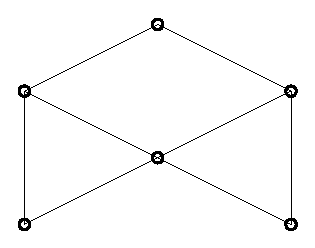
\includegraphics{fig/celula_correta.eps}
    \caption[Elemento conforme]{Elemento conforme}
    \label{fig:celula_correta}
\end{figure}


\begin{figure}
    \centering
    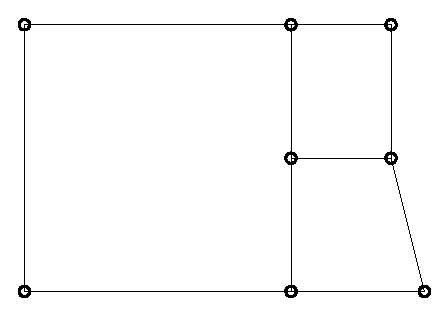
\includegraphics{fig/celula_errada.eps}
    \caption[Elemento não conforme]{Elemento não conforme}
    \label{fig:celula_errada}
\end{figure}

O objetivo da geração de malhas é criar elementos que se conformam com o formato e com a geometria do problema e obedeçam a restrições em seu tamanho e formato.

Nas malhas, tem-se que as fronteiras existem de modo a se poder aplicar as condições de contorno para a equação diferencial parcial e para permitir a descontinuidade nas propriedades físicas, como por exemplo diferenças na condutividade de calor. Uma fronteira, deve ser representada pela união de duas faces na malha. Elementos não podem cruzar essa fronteira, e no local onde dois materiais se encontram, suas malhas devem ter faces equivalentes. Esse requisito faz com que a geração de malhas seja mais difícil se o domínio possuir ângulos pequenos.

\subsection{Elementos desejados}
Um bom elemento de malha deve seguir várias restrições de modo a produzir um bom resultado numérico. Entre essas restrições está o formato dos elementos, que no caso de elemntos triangulares deve ser o mais equilátero possível de modo a diminuir erros de interpolação.

A triangulação de Delaunay para um conjunto de pontos discretos P em um plano é uma triangularização que faz com que nenhum ponto em P esteja dentro do circuncirculo de qualquer triangulo formado pelo algoritmo.

A triangularização de Delaunay maximiza o menor angulo de todos os ângulos criados pela triangularização. O nome desse método vem de Boris Delaunay em seu trabalho no tópico em 1934.

Para um conjunto de pontos em uma mesma linha, não existe triangularização de Delaunay (a noção de triangulo nesse caso é degenerada). Para quatro ou mais pontos em um mesmo círculo (por exemplo os vértices de um retânculo) a triangularização não é única, pois cada um dos possíveis triangulos que dividem o quadrado satisfazem a "condição de Delaunay", ie., a confição de que os circuncírculos de todos os triangulos tenham interiores vazios.

% PARTE DA PREPARAÇÃO DA PESQUISA
% ----------------------------------------------------------
\part{Preparação da pesquisa}
\chapter[VOLUMES FINITOS]{VOLUMES FINITOS}

\section{Introdução}

Na ciência e engenharia, modelos matemáticos são desenvolvidos de modo a ajudar a entender um dado fenômeno físico. Tais modelos frequentemente geram equações que contém alguma derivada de uma função desconhecida. Tais equações são chamadas de equações diferenciais. \cite{NagleR.KentB.SaffEdwardDavidSnider2012}.

Tais modelos matemáticos, desenvolvidos na área da mecânica dos fluídos, possuem como objetivo entender um fenômeno físico que nem sempre podemos medir ou observar, e portanto, compreender completamente. \cite{book}

Por outro lado, o desenvolvimento de uma ferramenta de simulação pressupõe que nós podemos entender um fenômeno físico bem o suficiente para modelá-lo. Felizmente, sabemos que todos os processos físicos são governados pelas mesmas leis de conservação universais.

Por exemplo, podemos não entender completamente as interações que geram fluxos de ar turbulentos em uma aeronave, mas sabemos que não importando a complexidade desse fenômeno, as leis de conservação de massa, momento (linear e angular) e energia existem.
Na maioria dos casos, as equações diferenciais parciais podem ser interpretadas como a manifestação dessas leis de conservação. Portanto, após a solução de tais equações em um domínio computacional, a solução final deve satisfazer as leis de conservação globalmente, assim como localmente.

O método dos volumes finitos é um método de discretização adequado para a simulação numérica de vários tipos de leis de conservação. Este método tem sido usado em muitos problemas na engenharia como na mecânica dos fluidos, transferência de calor e massa e na engenharia de petróleo.

Ele pode ser utilizado em geometrias arbitrárias usando-se malhas estruturadas ou não-estruturadas. Outra grande vantagem do método é a sua propriedade de conservação de fluxos entre uma célula e a sua vizinha, o que faz o método ser muito atrativo para problemas em que o fluxo de uma grandeza tem importância, como no caso da mecânica dos fluidos.

O método dos volume finitos, inicialmente, usava malhas estruturadas, no entanto, essas malhas estruturadas não são adequadas para muitas geometrias que aparecem na prática da engenharia, pois é muito difícil a geração de malhas estruturadas de boa qualidade com o refinamento adequado apenas onde for necessário para aumentar a acurácia da solução usando-se um número razoável de células. O método dos volumes finitos opera em células com qualquer formato, o que facilita o processo de geração de malhas, pois pode-se usar células com formatos arbitrários. \cite{doi:10.1080/10407791003685155}

\section{Conceitos de elementos e volumes de controle}

O conceito de elementos não é tradicionalmente usado no método de volumes finitos pois basta definir volumes de controle para a integração das equações governantes e posterior aproximações pertinentes ao processo de discretização. \cite{Versteeg2007}

Os elementos são sempre definidos em função da malha criada pelo gerador de malhas, o elemento é um ente geométrico que cobre todo o domínio computacional sem superposição e sem pedaços nas fronteiras.

Os volumes de controle são criados tendo-se por base os elementos criados. Existem duas classes básicas de métodos de determinação dos volumes de controle, baseadas na relatividade geométrica entre volumes e elementos:

\begin{itemize}
    \item Volumes centrado ou célula centrada (cell-centered): as informações (variáveis de interesse) são determinadas no centro (geométrico) do volume de controle, que coincide com o elemento de malha. Esta é a construção clássica de volumes finitos, em que os pontos de integração se localizam no centro das faces como na Figura \ref{fig:volume_centrado}
    \item Volume de controle baseado no vértice (vertex-based control volumes): o volume de controle é construído com seu centro coincidente a um nó da malha, ou seja, a um vértice do elemento de malha. Cada volume de controle é constituído por partes (subvolumes de controle) dos elementos vizinhos, aos quais pertence o nó empregado como centro do volume, onde são armazanadas as informações. Uma metodologia para geração dos volumes, conhecida como método das medianas, consiste em ligar os centroides dos elementos aos pontos médios de suas faces como na Figura \ref{fig:volume_vertice}
\end{itemize}

\begin{figure}[ht]
    \begin{subfigure}{.5\textwidth}
        \centering
        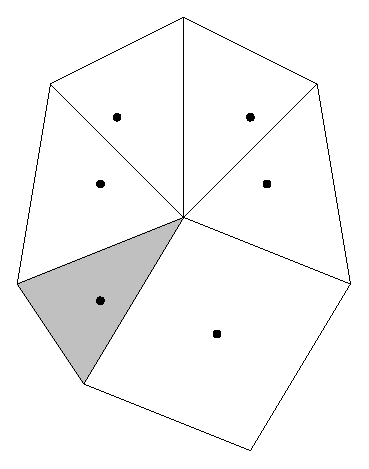
\includegraphics[width=.8\linewidth]{fig/volume_centrado.eps}
        \caption{Volume Centrado}
        \label{fig:volume_centrado}        
    \end{subfigure}
    \begin{subfigure}{.5\textwidth}
        \centering
        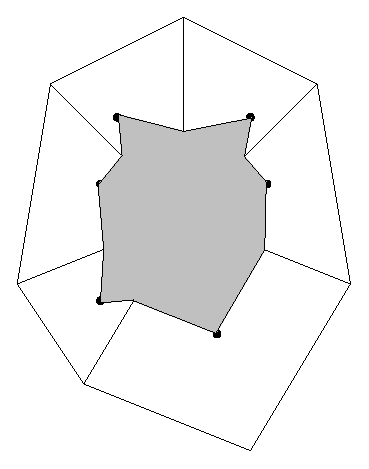
\includegraphics[width=.8\linewidth]{fig/volume_vertice.eps}
        \caption[]{Volume Baseado no vértice}
        \label{fig:volume_vertice}        
    \end{subfigure}

    \caption{Criação de Volumes de Controle}
    \label{fig:volume-controle}
\end{figure}

\section{Método dos Volumes Finitos para o problema da difusão 2D}

As equações governantes da mecânica dos fluidos, também chamadas de equações de Navier-Stokes são um conjunto de equações diferenciais que descrevem o escoamento de fluidos. Tais equações podem ser escritas de forma geral por uma equação de transporte:

\begin{equation}
    \int_{V_{CV}} \frac{\partial \rho \phi}{\partial t}dV + \int_{V_{CV}} \nabla \cdot (\rho \vec{U}\phi)dV - \int_{V_{CV}} \nabla \cdot (\rho \Gamma_\phi \nabla\phi)dV = \int_{V_{CV}} S_\phi(\phi)dV
\end{equation}

Em que $\phi$ é uma propriedade tensorial considerada contínua no espaço, $\Gamma_\phi$ é o coeficiente de difusão e $S_\phi(\phi)$ é o termo fonte. Nesse trabalho é considerado apenas o termo de difusão dessa equação, cuja discretização será apresentada a seguir.
\criarsimbolo{$ \phi $}{Propriedade Tensorial}
\criarsimbolo{$ \Gamma_\phi $}{Coeficiente de Difusão}
\criarsimbolo{$ S_\phi(\phi) $}{Termo Fonte}

O método dos volumes finitos é conservativo localmente porque ele é baseado em um balanço local escrito para cada célula de discretização, também chamada de "volume de controle". Se pegarmos uma equação de Poisson, temos que matematicamente, o lado esquerda dessa equação irá descrever um processo de difusão, enquanto que o lado direito descreve um processo de geração, por exemplo:

\begin{equation}
    \vec{q} = -k \nabla T
\end{equation}
$\vec{q}$ representa o fluxo de calor devido a diferença de temperatura
\criarsimbolo{$ \vec{q} $}{Fluxo de calor}

\begin{equation}
    \vec{J} = -D \nabla Y
\end{equation}
$\vec{J}$ representa o fluxo de massa devido a diferença de massa
\criarsimbolo{$ \vec{J} $}{Fluxo de Massa}

\begin{equation}             
    \vec{j} = -\sigma \nabla \phi
\end{equation}
$\vec{j}$ representa o fluxo de corrente devido a diferença de tensão
\criarsimbolo{$ \vec{j} $}{Fluxo de Corrente Elétrica}

Se agora, considerarmos a conservação de energia em um corpo sólido, e assumindo que:
\begin{itemize}
    \item O único modo de transferência de calor é por condução
    \item Não é realizado trabalho pelo ou sobre o sistema
    \item Estado estacionário
\end{itemize}

Nesse caso, podemos reduzir a conservação de energia em:

Taxa de transferência de calor para o volume de controle + taxa de calor gerado dentro do volume de controle = taxa de transferência de calor para fora do volume de controle.

Matematicamente, escrevemos como:

\begin{equation}
    \dot{Q_{in}} + \dot{Q_{gen}} = \dot{Q_{out}}
    \label{eq:2.4}
\end{equation}

Dado um volume $V_0$ com uma área de superfície $S$, podemos denotar $\vec{q}$ como o vetor de fluxo de calor (devido à condução) e $\vec{q} \cdot \vec{n}$ como a componente do vetor de fluxo normal a borda do volume.

Desse modo temos que $\int_S \vec{q}\cdot\hat{n}dA$ representa o total de calor sendo transferido pela fronteira do volume de controle $(\dot{Q_{out}} - \dot{Q_{in}})$ e, substituindo na equação de conservação da energia \ref{eq:2.4} temos:

\begin{equation}
    \dot{Q}_{gen} = \int_S \vec{q}\cdot\hat{n}dA = \int_V \dot{q}_{gen}dV
\end{equation}

Utilizando o teorema da divergência de Gauss podemos chegar a:

\begin{equation}
    \int_V \dot{q}_{gen}dV = \int_S \vec{q}\cdot\hat{n}dA = \int_V \nabla\cdot\vec{q}dV
\end{equation}

Combinando ambos os termos, temos:

\begin{equation}
    \int_V (\nabla \cdot \vec{q} - \dot{q}_{gen})dV = 0
\end{equation}

Como o termo dV não é igual a zero, isso implica em:

\begin{equation}
    \nabla \cdot \vec{q} - \dot{q}_{gen} = 0
    \label{difusao:poisson}
\end{equation}

Como, nesse caso o fluxo de calor é devido apenas a condução, podemos expressar ela em termos de temperatura usando a lei de Fourier da transferência de calor por condução, $\vec{q} = -k \nabla T$.

Substituindo na equação \ref{difusao:poisson} temos que:

\begin{equation}
    \nabla \cdot \vec{q} - \dot{q}_{gen} = \nabla \cdot (-k \nabla T) - \dot{q}_{gen} = 0
\end{equation}

Rearranjando:

\begin{equation}
    \nabla \cdot (k \nabla T) = -\dot{q}_{gen}
\end{equation}

Considere a seguinte equação de difusão na forma generalizada da equação de Poisson:

\begin{equation}
    \nabla \cdot (\Gamma \nabla \phi) = S_\phi
\end{equation}

Temos que $\Gamma$ é conhecido como a propriedade de transporte, e sendo um escalar, segue que:

\begin{equation}
    \Gamma \nabla \phi = \left( \Gamma \frac{\partial \phi}{\partial x} \vec{i} + \Gamma \frac{\partial \phi}{\partial y} \vec{j} + \Gamma \frac{\partial \phi}{\partial z} \vec{k} \right) = \vec{J}
\end{equation}

O fluxo é $\phi$

Segue agora que o divergente dessa expressão fica:

\begin{equation}
\begin{split}
    \nabla \cdot (\Gamma \nabla \phi) &= \left( \frac{\partial}{\partial x}\vec{i} + \frac{\partial}{\partial y}\vec{j} + \frac{\partial}{\partial z}\vec{k} \right) \cdot \left( \Gamma \frac{\partial \phi}{\partial x}\vec{i} + \Gamma \frac{\partial \phi}{\partial y}\vec{j} + \Gamma \frac{\partial \phi}{\partial z}\vec{k} \right)\\
    &= \frac{\partial}{\partial x} \left( \Gamma \frac{\partial \phi}{\partial x} \right) + \frac{\partial}{\partial y} \left( \Gamma \frac{\partial \phi}{\partial y} \right) + \frac{\partial}{\partial z} \left( \Gamma \frac{\partial \phi}{\partial z} \right)
\end{split}
\end{equation}

Portanto, a equação inicial, em coordenadas cartesianas, pode ser escrita como:

\begin{equation}
    \frac{\partial}{\partial x} \left( \Gamma \frac{\partial \phi}{\partial x} \right) + \frac{\partial}{\partial y} \left( \Gamma \frac{\partial \phi}{\partial y} \right) + \frac{\partial}{\partial z} \left( \Gamma \frac{\partial \phi}{\partial z} \right) = S_\phi
\end{equation}

Ou de forma resumida voltando para o exemplo da transferência de calor:

\begin{equation}
    \nabla^2 T= -\frac{\dot{q}_{gen}}{k}
\end{equation}

No método dos volumes finitos, deve-se integrar a equação governante sobre um volume de controle antes de se fazer as aproximações das derivadas. Desse modo temos:

\begin{equation}
    \int_{V_0} \nabla \cdot (\Gamma \nabla \phi) dV = \int_{V_0} S_\phi dV
\end{equation}

Se agora aplicarmos o teorema da divergência de Gauss no lado esquerdo dessa equação, temos:

\begin{equation}
    \int_{V_0} \nabla \cdot (\Gamma \nabla \phi) dV = \int_{V_0} \nabla \cdot (\vec{J}) dV = \int_S \vec{J} \cdot \hat{n} dA
\end{equation}

Sendo $\vec{J}$ um vetor de fluxo e $\hat{n}$ é um vetor normal que aponta para fora do elemento de área $dA$.

No método de volumes finitos, todas as informações são armazenadas no centro das células.

Uma hipótese crítica que deve ser aceita, é a de que o valor da quantidade analisada nesse interior da célula é igual a média dessa quantidade em todo o volume.

Sob essa hipótese, temos que a média de $S_\phi$ no volume pode ser adquirida com o seu valor no centro da célula, portanto:

\begin{equation}
    \int_{V_0} S_\phi dV \approx S_{\phi,0} V_0
\end{equation}

O resultado final da expressão é dado por:

\begin{equation}
    \int_S (\Gamma \nabla \phi) \cdot \hat{n} dA = S_{\phi,0} V_0
\end{equation}

Essa equação para volumes finitos é válida para um volume de controle de formato arbitrário, nota-se que essa é na verdade uma equação integral e portanto é chamada de forma fraca da equação.

No contexto da resolução desse método computacionalmente, temos que os volumes de controle são limitados por um número finito de faces planas (em 3D) ou de faces lineares (em 2D). Portanto temos que a integral pode ser substituida por uma soma discreta sobre essas faces, resultando em:

\begin{equation}
    \sum_f \vec{J} \cdot \hat{n}_f A_f = \sum_f \Gamma_f (\nabla \phi)_f \cdot \hat{n}_f A_f = S_{\phi,0} V_0
\end{equation}

Nota-se que não é feita nenhuma consideração com relação ao formato ou tamanho do volume de controle.

De modo a continuar com a discretização da equação, deve-se aproximar o gradiente de $\phi$ em termos dos valores de $\phi$ no centro da célula, para isso usa-se a seguir um exemplo de um pedaço de uma malha como na Figura \ref{fig:fig1}.

Considerando a malha da Figura \ref{fig:fig1}, tem-se que a equação expandida fica como:

\begin{figure}
    \centering
    \caption{Grade para o FVM}
    \includegraphics{fig/Figura1}
    \label{fig:fig1}    
\end{figure}

\begin{equation}
    \Gamma_e (\nabla \phi)_e \cdot \hat{n}_e A_e + \Gamma_w (\nabla \phi)_w \cdot \hat{n}_w A_w + \Gamma_n (\nabla \phi)_n \cdot \hat{n}_n A_n + \Gamma_s (\nabla \phi)_s \cdot \hat{n}_s A_s = S_{\phi,0} V_0
\end{equation}

Para essa malha, temos que:

\begin{eqnarray}
    V_0 =& \Delta x \Delta y\\
    A_e =& A_w = \Delta y\\
    A_n =& A_s = \Delta x
\end{eqnarray}

Também podemos dizer:

\begin{eqnarray}
    \hat{n}_e =& \hat{i}\\
    \hat{n}_w =& -\hat{i}\\
    \hat{n}_n =& \hat{j}\\
    \hat{n}_s =& -\hat{j}
\end{eqnarray}

Considerando a definição de gradiente, chegamos a:

\begin{equation}
    (\nabla \phi)_e \cdot \hat{n}_e = \left( \frac{\partial \phi}{\partial x} \hat{i} + \frac{\partial \phi}{\partial y} \hat{j} + \frac{\partial \phi}{\partial z} \hat{k} \right) \cdot \hat{i} = \left( \frac{\partial \phi}{\partial x} \right)_e
\end{equation}

Temos um termo similar para os outros três termos.

Logo a equação governante fica como:

\begin{equation}
    \label{eq:2.29}
    \Gamma_e \left( \frac{\partial \phi}{\partial x} \right)_e \Delta y - \Gamma_w \left( \frac{\partial \phi}{\partial x} \right)_w \Delta y + \Gamma_n \left( \frac{\partial \phi}{\partial x} \right)_n \Delta x - \Gamma_s \left( \frac{\partial \phi}{\partial x} \right)_e \Delta x = S_{\phi,0} \Delta x \Delta y
\end{equation}

O próximo passo é expressar as quantidades nas faces (e,w,n,s) em termos das quantidades nos centros das células (E,W,N,S).

Normalmente, de modo a se obter o coeficiente de transporte nas faces, usa-se uma interpolação linear, para uma malha uniforme para a face e, fica como:

\begin{equation}
    \Gamma_e = \frac{\Gamma_E + \Gamma_O}{2}
\end{equation}

Para expressar a derivada de primeira ordem em termos de valores no centro das células, é empregado a expansão em série de Taylor:

\begin{equation}
    \label{eq:8}
    \phi_E = \phi_e + \frac{\Delta x}{2} \frac{\partial \phi}{\partial x} \bigg|_e + \frac{(\Delta x / 2)^2}{2!} \frac{\partial^2 \phi}{\partial x^2} \bigg|_e + \frac{(\Delta x / 2)^3}{3!} \frac{\partial^3 \phi}{\partial x^3} \bigg|_e + ...
\end{equation}

\begin{equation}
    \label{eq:9}
    \phi_O = \phi_e - \frac{\Delta x}{2} \frac{\partial \phi}{\partial x} \bigg|_e + \frac{(\Delta x / 2)^2}{2!} \frac{\partial^2 \phi}{\partial x^2} \bigg|_e - \frac{(\Delta x / 2)^3}{3!} \frac{\partial^3 \phi}{\partial x^3} \bigg|_e + ...
\end{equation}

Subtraindo \ref{eq:9} de \ref{eq:8} chegamos a:

\begin{equation}
    \label{eq:10}
    \phi_E - \phi_O = \Delta x \frac{\partial \phi}{\partial x} \bigg|_e + \frac{(\Delta x / 2)^3}{3} \frac{\partial^3 \phi}{\partial x^3} \bigg|_e + ...
\end{equation}

Rearranjando a equação \ref{eq:10} chegamos no chamado "Central Difference scheme":

\begin{equation}
    \label{eq:11}
    \frac{\partial \phi}{\partial x} \bigg|_e = \frac{\phi_E - \phi_O}{\Delta x} - \frac{(\Delta x)^2}{24} \frac{\partial^3 \phi}{\partial x^3} \bigg|_e + ...
\end{equation}

Nota-se que essa aproximação é de segunda ordem.

Substituindo a expressão para a aproximação numérica da derivada de primeira ordem e os coeficientes de transporte na equação governante discretizada pelo método dos volumes finitos temos:

\begin{equation}
    \begin{split}
    \label{eq:12}
    &\frac{\Gamma_E + \Gamma_O}{2} \left( \frac{\phi_E - \phi_O}{\Delta x} \right) \Delta y - \frac{\Gamma_W + \Gamma_O}{2} \left( \frac{\phi_O - \phi_W}{\Delta x} \right) \Delta y + \frac{\Gamma_N + \Gamma_O}{2} \left( \frac{\phi_N - \phi_O}{\Delta y} \right) \Delta x\\
    &- \frac{\Gamma_S + \Gamma_O}{2} \left( \frac{\phi_O - \phi_S}{\Delta y} \right) \Delta x = S_{\phi,0} \Delta x \Delta y
    \end{split}
\end{equation}

A equação \ref{eq:12} pode ser reescrita em um formato que irá gerar uma matriz penta-diagonal no seguinte formato:

\begin{equation}
    a_P \phi_P = a_W \phi_W + a_E \phi_E + a_N \phi_N + a_S \phi_S - b_P
\end{equation}

Cujos coeficientes são:

\begin{eqnarray}
    a_P =& \left( \frac{\Gamma_E + \Gamma_O}{2 \Delta x} \Delta y + \frac{\Gamma_W + \Gamma_O}{2 \Delta x} \Delta y + \frac{\Gamma_N + \Gamma_O}{2 \Delta y} \Delta x + \frac{\Gamma_S + \Gamma_O}{2 \Delta y} \Delta x \right)\\
    a_E =& \frac{\Gamma_E + \Gamma_O}{2 \Delta x} \Delta y\\
    a_W =& \frac{\Gamma_W + \Gamma_O}{2 \Delta x} \Delta y\\
    a_N =& \frac{\Gamma_N + \Gamma_O}{2 \Delta y} \Delta x\\
    a_S =& \frac{\Gamma_S + \Gamma_O}{2 \Delta y} \Delta x\\
    b_P =& S_{\phi,0} \Delta x \Delta y
\end{eqnarray}

Se for considerado uma condição de contorno de Dirichlet, teremos, conforme a Figura  \ref{fig:fig2} onde $w$ é conhecido:

\begin{figure}[h!]
    \centering
    \includegraphics[width=0.4\linewidth]{fig/Figura2.eps}
    \caption{Condições de contorno}
    \label{fig:fig2}
\end{figure}

Nesse caso teremos que a aproximação numérica da derivada com relação a face $w$ não pode mais ser feita com CDS-2 pois não existe outra célula a oeste dessa.

Pode-se então usar a aproximação DDS-4 para essa derivada de modo a manter a equação com um erro de segunda ordem.

\begin{equation}
    \label{eq:2.43}
    \frac{\partial \phi}{\partial x} \bigg|_w = \frac{9 \phi_O - \phi_{E} -8\phi_w}{3 \Delta x} + \frac{(\Delta x)^2}{9} \frac{\partial^3 \phi}{\partial x^3} \bigg|_w + ...
\end{equation}

Substituindo agora a equação \ref{eq:2.43} que é a expressão para a derivada do fluxo em relação a $x$ na face $w$ na equação \ref{eq:2.29} tem-se:

\begin{equation}
    \label{eq:2.44}
    \left\{ \Gamma \frac{\partial \phi}{\partial x}\bigg|_e -\Gamma \frac{\partial \phi}{\partial x}\bigg|_w  \right\} \Delta y + \left\{\Gamma \frac{\partial}{\partial y}\bigg|_n - \Gamma \frac{\partial \phi}{\partial y}\bigg|_s  \right\} \Delta x = S_{\phi,o}\Delta x \Delta y
\end{equation}

\begin{equation}
    \label{eq:2.45}
    \left\{\Gamma_e \frac{\Phi_E-\Phi_O}{\Delta x} - \Gamma_w \frac{9 \phi_O - \phi_{E} -8\phi_w}{3 \Delta x} \right\} \Delta y + \left\{\Gamma_n \frac{\Phi_N-\Phi_O}{\Delta y} - \Gamma_s \frac{\Phi_O-\Phi_S}{\Delta y}  \right\} \Delta x = S_{\phi,o}\Delta x \Delta y
\end{equation}

Rearranjando-se a equação \ref{eq:2.45} e aplicando a condição de contorno $\phi_w = \phi_{left}$ temos:

\begin{equation}
\begin{split}
    &\left[\left( \frac{\Gamma_e}{\Delta x}+\frac{3\Gamma_w}{\Delta x}\right)\Delta y  + \left(\frac{\Gamma_n}{\Delta y}+\frac{\Gamma_w}{\Delta y}\right)\Delta x  \right]\phi_O\\
    - &\left[\left(\frac{\Gamma_e}{\Delta x}+\frac{\Gamma_w}{3\Delta x}\right)\Delta y\right]\phi_E\\
    - & \left[\left(\frac{\Gamma_n}{\Delta y}\right)\Delta x\right]\phi_N-\left[\left(\frac{\Gamma_s}{\Delta y}\right)\Delta x\right]\phi_S = S_{\phi,o}\Delta x \Delta y + \left[\frac{8\Gamma_w \Delta y}{3 \Delta x}\right]\phi_w
\end{split}
\end{equation}

Nesse caso teremos que a matriz da equação com relação a essa condição de contorno continuará sendo penta-diagonal, e a informação da condição de contorno ficará no termo fonte correspondente.

Já para o caso da condição de contorno de Neumann, teremos apenas que substituir na equação \ref{eq:2.29} o valor para o fluxo correspondente que já é conhecido.

\section{Análise de erros no método dos volumes finitos}

Na solução do FVM temos que considerar o erro de discretização gerado, essa estimativa de erro já foi realizado várias vezes e existe na literatura como em \cite{Jasak1996} e \cite{Muzaferija2014}.

Segundo \cite{Juretic2004} tanto a qualidade da malha quanto o formato da célula utilizado influenciam na acurácia da solução, que varia para o termo convectivo e difusivo da equação diferencial a ser solucionada.

Na discretização do método dos volumes finitos, uma importante propriedade necessária dessa discretização é que a solução encontrada deve tender à solução exata dado que o número de volumes de controle tenda ao infinito. Para isso ocorrer deve-se satisfazer os seguintes requisitos:
\begin{itemize}
    \item \textbf{Consistência:} O erro de discretização na solução numérica deve tender a zero a medida que o espaçamento da malha tenda a zero.
    \item \textbf{Estabilidade:} A discretização é considerada estável se ela não aumenta nenhum erro durante o processo de cálculo.
    \item \textbf{Concervação:} O FMV é obtido com a integração da equação diferencial governante e, portanto, para propriedades conservativas deve obedecer às mesmas leis de conservação da equação diferencial.
    \item \textbf{Limitação:} Algumas propriedades físicas ficam entre certas fronteiras, por exemplo a densidade nunca é negativa, logo deve-se ter como requisito que a discretização não gere valores impossíveis na física.
\end{itemize}
\cite{Juretic2004}

Nese trabalho é considerado apenas as malhas 2D com o formato de célula triangular pois este é muito comum e mais facilmente implementado, outra limitação desse trabalho é que é considerado apenas o termo difusivo.

Conforme foi mostrado, a partir da equação \ref{eq:2.29}, as derivadas dessa equação são aproximadas usando-se a geometria da malha, no caso com uma célula quadrada. Logo tem-se que o formato da célula influencia na acurácia da solução. A partir da geometria da malha, pode-se gerar as seguintes propriedades:

\begin{itemize}
    \item \textbf{Não Ortogonalidade:} Conforme a Figura \ref{nao-ortogo} pode-se definir a não Ortogonalidade como o angulo $\theta$ entre o vetor $\vec{d}=\vec{PA}$ e o vetor normal a face ab $\hat{n}$. Esse angulo deve ser o menor possível. A razão será discutida posteriormente.
    \item \textbf{Assimetria de malha:} Quando o vetor d não intercepta a face ab no seu centro, a célula de malha é definida como assimétria conforme a Figura \ref{fig:assimetria}. O grau de assimetria pode ser definido como $\Psi = \frac{|m|}{|d|}$
    \item \textbf{Uniformidade:}  Uma malha é uniforme quando o vetor $\vec{d}$ intercepta a face no meio entre os nós $P$ e $A$. A uniformidade pode ser medida como:
    \begin{equation*}
        f_x = \frac{|x_{fi}-x_N|}{|d|}
    \end{equation*}
    portanto $f_x=0.5$ é o valor para uma malha uniforme. Esta propriedade afeta a acurácia dos termos de gradiente.
\end{itemize}

\begin{figure}
    \begin{subfigure}{.5\textwidth}
        \centering
        \caption{Não Ortogonalidade}
        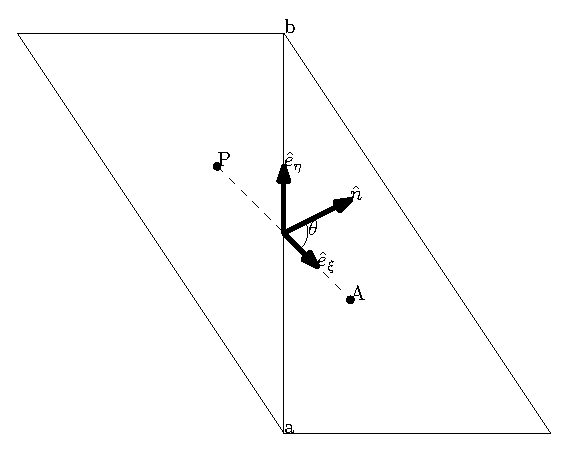
\includegraphics[width=.8\linewidth]{fig/nao-ortogo}
        \label{nao-ortogo}
    \end{subfigure}
    \begin{subfigure}{.5\textwidth}
        \centering
        \caption{Assimetria}
        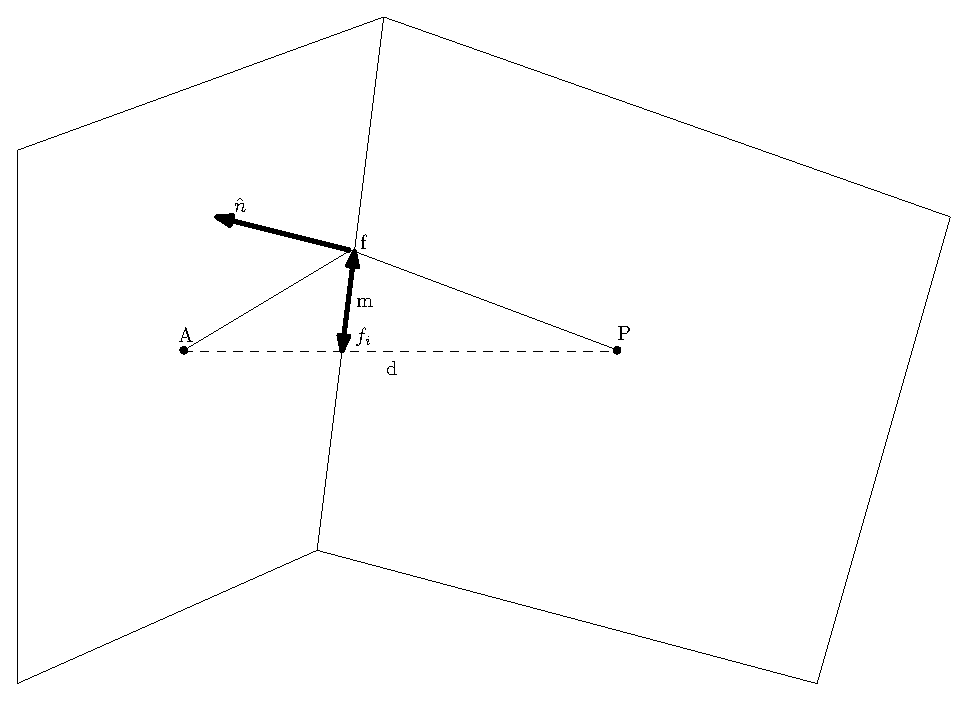
\includegraphics[width=.8\linewidth]{fig/assimetria.eps}
        \label{fig:assimetria}
    \end{subfigure}

    \caption{Erros no volume finito}
\end{figure}

\section{Termo de Difusão}

A partir da equação \ref{eq:2.29} considerando-se o termo de difusão, aplicando-se o teorema da divergência de Gauss e a aproximação de que os gradientes nas faces são constantes (assumindo-se uma variação linear da propriedade $\phi$) chega-se a:

\begin{equation}
    \int_{V_P} \nabla \cdot (\rho \Gamma_\phi \nabla\phi)dV = \sum_f \vec{S} \cdot (\rho \Gamma_\phi \nabla \phi)_f = \sum (\rho \Gamma_\phi)_f (\vec{S} \cdot \nabla \phi)_f
\end{equation}

Onde o vetor $\vec{S}$ está na Figura \ref{fig:non-orthogonality}

\begin{figure}[]
    \centering
    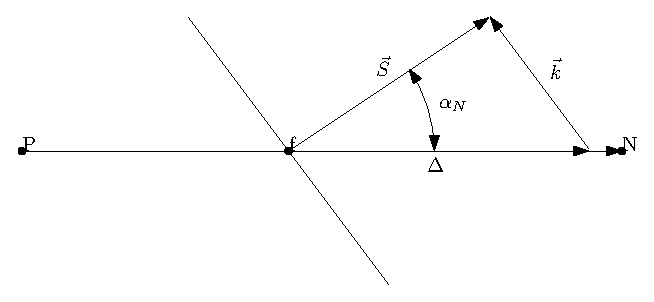
\includegraphics{fig/non-orthogonality.eps}
    \caption{Erro do termo difusivo em malha não ortogonal}
    \label{fig:non-orthogonality}
\end{figure}

% O termo $(\rho \Gamma_\phi)_f$ é interpolado nas faces usando-se a equação \ref{eq:2.49}. Onde $\phi_{f_i}$ e $(\nabla \phi)_{f_i}$ são os valores de $\phi$ e $\nabla \phi$ no ponto onde o vetor $\vec{d}$ intercepta a face conforme a Figura \ref{fig:assimetria}.

% \begin{equation}
%     \phi_f = \phi_{f_i} = \vec{m} \cdot (\nabla \phi)_{f_i}
%     \label{eq:2.49}
% \end{equation}

% Já o termo $(\vec{S} \cdot \nabla \phi)_f$ é aproximado usando-se a seguinte equação:

% \begin{equation}
%     (\vec{S} \cdot \nabla \phi)_f = 
% \end{equation}

Segundo a dedução encontrada em \cite{Juretic2004} a ordem do erro do termo de difusão é igual a menor entre a ordem do erro de interpolação e do erro de discretização do termo gradiente dados por:

\begin{equation}
    e_{interpolation} = -\frac{1}{2} |\vec{d^2}| (f_x(1-f_x)(\hat{d^2}:(\nabla \nabla \phi)_{f_i} + \psi |\vec{d}| \hat{m} \cdot (\hat{d^2} : (\nabla \nabla \nabla \phi)_{f_i})) + \frac{\psi^2}{2} |\vec{d^2}| (\hat{m^2} : (\nabla \nabla \phi)_{f_i}) )
    \label{eq:2.49}
\end{equation}

\begin{equation}
    e_{snGrad} = -\frac{|\vec{S}|}{6 \cot{\alpha_N}} |\vec{d^2}| ((1-f_x)^3 + f_x^3)\hat{d^3}:: (\nabla \nabla \nabla \phi)_f - |\vec{S}| \tan{\alpha_N} \frac{|\vec{d^2}|}{2}f_x(1-f_x)\hat{k} \cdot (\hat{d^2}:(\nabla \nabla \nabla \phi)_f)
    \label{eq:2.50}
\end{equation}

Onde $\hat{d}$ e $\hat{k}$ são vetores unitários nas direções de $\vec{d}$ e $\vec{k}$ respectivamente. Verifica-se da equação \ref{eq:2.50} que essa será de primeira-ordem exceto para o valor de $f_x=0.5$, ou seja, para uma malha uniforme. Logo para uma malha uniforme a aproximação se torna de segunda-ordem. O erro também depende do ângulo $\alpha_N$ e será mínimo quando $\alpha_N=0$, ou seja, quando a malha for ortogonal.
\chapter[TRANSFORMAÇÃO DE COORDENADAS]{TRANSFORMAÇÃO DE COORDENADAS}

Na transformação de coordenadas, é necessário conhecer em quais parâmetros estão embutidas as informações da forma e do tamanho real do domínio de cálculo. \cite{Maliska2004} Existem duas abordagens na transformação de coordenadas:
\begin{itemize}
    \item o sistema de coordenada local (relacionado a malhas não-estruturadas)
    \item sistema de coordenadas global (relacionado a malhas estruturadas)
\end{itemize}

Seja $f=f(\xi, \eta)$, onde $f$ reqpresenta $x,y,T$\dots
Neste caso:

\begin{equation}
    \frac{\partial f}{\partial x} = \frac{\partial f}{\partial \xi}\frac{\partial \xi}{\partial x}+\frac{\partial f}{\partial \eta}\frac{\partial \eta}{\partial x}
    \label{eq:3.1}
\end{equation}
\begin{equation}
    \frac{\partial f}{\partial y} = \frac{\partial f}{\partial \xi}\frac{\partial \xi}{\partial y}+\frac{\partial f}{\partial \eta}\frac{\partial \eta}{\partial y}
    \label{eq:3.2}
\end{equation}

Fazendo $f=x$ na equação \ref{eq:3.1} e $f=y$ na equação \ref{eq:3.2}, obtém-se:
\begin{equation*}
    1 = x_\xi \xi_x + x_\eta \eta_x\\
    0 = y_\xi \xi_x + y_\eta \eta_x
\end{equation*}

Resolvendo o sistema anterior encontra-se:
\begin{equation}
    \label{eq:3.3}
    \xi_x = y_\eta J
\end{equation}
\begin{equation}
    \label{eq:3.4}
    \eta_x = -y_\xi J
\end{equation}

\begin{equation}
    J = (x_\xi y_\eta - x_\eta y_\xi)^(-1)
    \label{eq:3.5}
\end{equation}

Onde na equação \ref{eq:3.5} $J$  é o jacobiano da transformação do sistema de coordenadas.

Agora, fazendo-se $f=x$ em \ref{eq:3.2} e $f=y$ em \ref{eq:3.2}, tem-se:
\begin{equation*}
    0 = x_xi \xi_y + x_\eta \eta_y
    1 = y_\xi \xi_y + y_\eta \eta_y
\end{equation*}

Ao se resolver o sistema anterior, obtém-se:
\begin{equation}
    \label{eq:3.6}
    \xi_y = -x_\eta J
\end{equation}
\begin{equation}
    \label{eq:3.7}
    \eta_y = x_\xi J
\end{equation}

A matriz jacobiana da transformação de coordenadas é definida por:
\begin{equation}
    \label{eq:3.8}
    J =
    \begin{bmatrix}
        \xi_x & \xi_y\\
        \eta_x & \eta_y
    \end{bmatrix}
    = (\xi_x \eta_y - \xi_y \eta_x)
\end{equation}

Tanto o Jacobiano quanto as métricas de transformação $(\xi_x, \xi_y, \eta_x, \eta_y)$ aparecerão nas equações diferenciais quando estas forem transformadas para o novo sistema de coordenadas $(\xi,\eta)$.

Como os domínios são discretos, existem dificuldades em se calcular as métricas da transformação direta $(\xi_x, \xi_y, \eta_x, \eta_y)$. Exemplo:

$\xi_x=\frac{\partial \xi}{\partial x}$ é necessário conhecer a variação $\partial x$ em uma linha de $y$ constante.

Desde modo, para se contornar esta dificuldade, utilizam-se as métricas da transformação inversa $(x_\xi, x_\eta, y_\xi, y_\eta)$, uma vez que no espaço transformado $(\xi, \eta)$ todas as coordenadas são conhecidas a priori.

As relações entre as métricas da transformação direta e inversa são dadas pelas equações \ref{eq:3.3} e \ref{eq:3.4}, \ref{eq:3.6} e \ref{eq:3.7}.

O jacobiano da transformação inversa é dado por:

\begin{equation}
    \label{eq:3.9}
    J^{-1} =
    \begin{vmatrix}
        x_\xi & x_\eta\\
        y_\xi & y_\eta
    \end{vmatrix}
    = (x|xi y_\eta - x|eta y_xi)
\end{equation}

Substituindo-se as equações \ref{eq:3.3}, \ref{eq:3.4}, \ref{eq:3.6} e \ref{eq:3.7} na equação \ref{eq:3.9}, prova-se que:

\begin{equation}
    \label{eq:3.10}
    J = \frac{1}{J^{-1}}
\end{equation}

Conforme a Figura \ref{Figura9} podemos chegar nas seguintes relações:

\begin{figure}[]
    \centering
    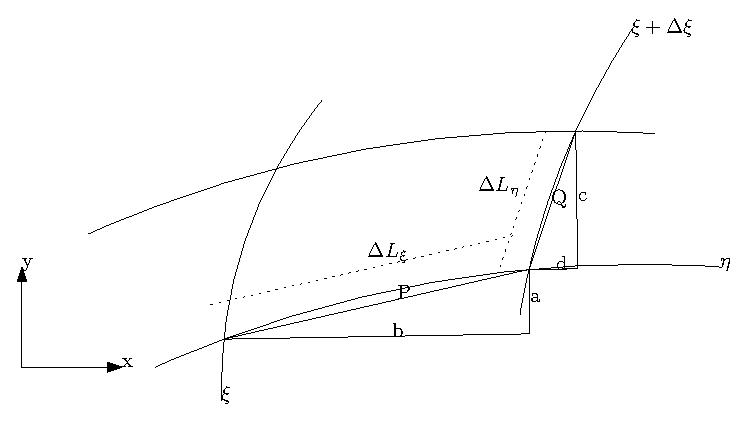
\includegraphics{fig/transformacao.eps}
    \caption{Transformação de Coordenadas}
    \label{Figura9}
\end{figure}

\begin{equation*}
    x_\xi \vert_P = \frac{x(\xi+\Delta \xi)-x(\xi)}{\Delta \xi} = \frac{b}{\Delta \xi}
\end{equation*}

Ou seja, $b=x_\xi \Delta \xi$

\begin{equation*}
    y_\xi \vert_P = \frac{y(\xi+\Delta \xi)-y(\xi)}{\Delta \xi} = \frac{a}{\Delta \xi}    
\end{equation*}

Ou seja, $a=y_\xi \Delta \xi$

\begin{equation*}
    \Delta L_\xi = \sqrt{a^2+b^2} = \sqrt{y_\xi^2 \Delta_\xi^2 + x_\xi^2+\Delta_\xi^2} = \Delta \xi \sqrt{x_\xi^2 + y_\xi^2}
\end{equation*}

Ou, escrito de outro modo:

\begin{equation}
    \label{eq:3.11}
    \Delta_\xi = \Delta \xi \sqrt{\gamma}
\end{equation}

em que:

\begin{equation}
    \label{eq:3.12}
    \gamma = x_\xi^2 + y_\xi^2
\end{equation}

\begin{equation*}
    y_\eta \vert_Q = \frac{y(\eta+\Delta \eta)-y(\eta)}{\Delta \eta} = \frac{c}{\Delta \eta}
\end{equation*}

Ou seja, $c=y_\eta \Delta_\eta$
\begin{equation*}
    x_\eta \vert_Q = \frac{x(\eta+\Delta \eta)-x(\eta)}{\Delta \eta} = \frac{d}{\Delta \eta}
\end{equation*}

Ou seja, $d=x_\eta \Delta_\eta$

\begin{equation*}
    \Delta L_\eta = \sqrt{c^2+d^2} = \sqrt{y_\eta^2 \Delta_\eta^2 + x_\eta^2+\Delta_\eta^2} = \Delta \eta \sqrt{x_\eta^2 + y_\eta^2}
\end{equation*}

Ou, escrito de outro modo:

\begin{equation}
    \label{eq:3.13}
    \Delta L_\eta = \Delta \eta \sqrt{\alpha}
\end{equation}

em que:

\begin{equation}
    \label{eq:3.14}
    \alpha = x_\eta^2 + y_\eta^2
\end{equation}

Para o cálculo da área formada por $\Delta L_\eta$ e $\Delta L_\xi$ temos, conforme a Figura \ref{fig:area}.

\begin{figure}[]
    \centering
    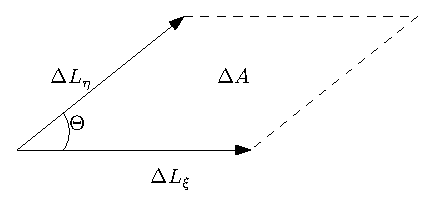
\includegraphics{fig/area.eps}
    \caption{Área}
    \label{fig:area}
\end{figure}

\begin{equation*}
    \Delta \vec{A} =
    \begin{vmatrix}
        \hat{i} & \hat{j} & \hat{k}\\
        x_\xi \Delta \xi & y_\xi \Delta \xi & 0\\
        x_\eta \Delta \eta & y_\eta \Delta -\eta & 0
    \end{vmatrix}
    = (x_\xi \Delta \xi y_\eta \Delta \eta - x_\eta \Delta \eta y_\xi \Delta \xi)\hat{k}
\end{equation*}

Assim:

\begin{equation*}
    \Delta A = x_\xi y_\eta \Delta \xi \Delta \eta - x_\eta y_\xi \Delta \xi \Delta \eta
\end{equation*}
\begin{equation*}
    \Delta A = (x_\xi y_\eta - x_\eta y_\xi)\Delta \xi \Delta \eta = J^{-1} \Delta \xi \Delta \eta\\
\end{equation*}    
\begin{equation}
    \label{eq:3.15}
    \Delta A = \frac{\Delta \xi \Delta \eta}{J}
\end{equation}

No caso tridimensional, pode-se provar que o volume físico $(\Delta v)$ é dado por:
\begin{equation}
    \label{eq:3.16}
    \Delta v = \frac{\Delta \xi \Delta \eta \Delta \gamma}{J}
\end{equation}

Sendo o jacobiano dado por:

\begin{equation}
    \label{eq:3.17}
    J = [x_\xi(y_\eta z_\gamma - y_\gamma z_\eta) - x_\eta(y_xi z_\gamma - y_\gamma z_\xi) + x_\gamma(y_\xi z_\eta - y_\eta z_\xi)]^{-1}
\end{equation}

\section{Tensor métrico 2D}

O Tensor métrico 2D é definido como:

\begin{equation}
    \label{eq:3.18}
    [g_{ij}] =
    \begin{vmatrix}
        g_{11} & g_{12}\\
        g_{21} & g_{22}
    \end{vmatrix}
    =
    \begin{vmatrix}
        \gamma & \beta\\
        \beta & \alpha
    \end{vmatrix}
\end{equation}

Em que:

\begin{equation}
    \label{eq:3.19}
    \beta = x_\xi x_\eta + y_\xi y_\eta
\end{equation}

Pode-se mostrar que o determinante do tensor métrico $g$ é dado por:

\begin{equation}
    \label{eq:3.20}
    g = \frac{1}{J^2}
\end{equation}

Das equações \ref{eq:3.20} e \ref{eq:3.18}, tem-se que:

\begin{equation*}
    \alpha \gamma - \beta^2 = \frac{1}{J^2}
\end{equation*}

E da equação \ref{eq:3.15}:

\begin{equation*}
    J=\frac{\Delta \xi \Delta \eta}{\Delta A}
\end{equation*}


Nesse caso,

\begin{equation*}
    \alpha \gamma - \beta^2 = \frac{\Delta A^2}{\Delta \xi^2 \Delta \eta^2}
\end{equation*}

Logo:

\begin{equation*}
    \Delta A^2 = (\alpha \gamma - \beta^2)\Delta \xi^2 \Delta \eta^2
\end{equation*}

Contudo,

\begin{equation*}
    \Delta A = \Delta L_\xi \Delta L_\eta \sin{\Theta} = \Delta \xi \sqrt{\gamma} \Delta \eta \sqrt{\alpha} \sin{\Theta}
\end{equation*}

Então:
\begin{equation*}
    \Delta A^2 = \Delta \xi^2 \gamma \Delta \eta^2 \alpha \sin{\Theta}^2
\end{equation*}

Igualando-se as expressões para $\Delta A^2$:
\begin{equation*}
    (\alpha \gamma - \beta^2)\Delta\xi^2 \Delta \eta^2 = \Delta \xi^2 \gamma \Delta \eta^2 \alpha \sin{\Theta}^2
\end{equation*}
\begin{equation*}
    \alpha \gamma - \beta^2 = \alpha \gamma \sin{\Theta}^2
\end{equation*}
\begin{equation*}
    \alpha \gamma(1-\sin{\Theta}^2) = \beta^2
\end{equation*}
\begin{equation*}
    \alpha \gamma \cos{\Theta}^2 = \beta^2
\end{equation*}

Ou seja:
\begin{equation}
    \label{eq:3.21}
    \beta = \sqrt{\alpha \gamma}\cos{\Theta}
\end{equation}

No caso de sistema ortogonais, $\Theta = \pi/2 = 90º$ e, portanto, $\beta = 0$. Deste modo, $\beta$ representa a não-ortogonalidade do sistema de coordenadas curvilíneas. O valor de $\Theta$ pode ser obtido para qualquer volume de controle ou malha, uma vez que ele é função de $\alpha, \beta$ e $\gamma$ que são funções das métricas.

\section{Vetores de base covariantes}
São os vetores tangentes às linhas de $\xi$ e $\eta$.

Conforme a Figura \ref{fig:e_xi} tem-se que:

\begin{equation}
    \label{eq:3.22}
    \vec{r} = x \hat{i} + y \hat{j}
\end{equation}

\begin{figure}[h]
    \centering
    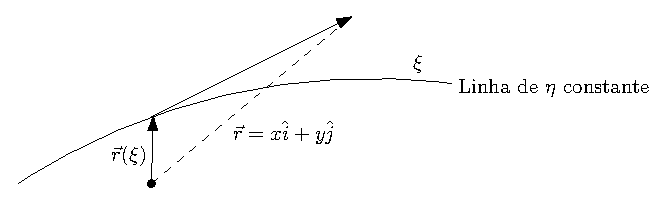
\includegraphics{fig/e_xi.eps}
    \caption{Definição de $e_\xi$}
    \label{fig:e_xi}
\end{figure}

\begin{equation}
    \label{eq:3.23}
    \vec{e_\xi} = \lim_{\Delta \xi \to 0} \frac{\vec{r}(\xi + \Delta \xi) - \vec{r}(\xi)}{\Delta \xi} = \frac{\partial \vec{r}}{\partial \xi}
\end{equation}

Portanto,

\begin{equation}
    \label{eq:3.24}
    \vec{e_\xi} = x_\xi \hat{i} + y_\xi \hat{j}
\end{equation}

que é tangente à linha de $\eta$ constante e analogamente:

\begin{equation}
    \label{eq:3.25}
    \vec{e_\eta} = x_\eta \hat{i} + y_\eta \hat{j}
\end{equation}

que é tangente à linha de $\xi$ constante.

Nota-se que, como $\hat{i}$ e $\hat{j}$ são unitários, $\vec{e_\xi}$ e $\vec{e_\eta}$ não o são.

\begin{equation}
    \label{eq:3.26}
    \vec{e_\xi} \cdot \vec{e_\xi} = x_\xi^2 + y_\xi^2 = \gamma
\end{equation}

\begin{equation}
    \label{eq:3.27}
    \vec{e_\eta} \cdot \vec{e_\eta} = x_\eta^2 + y_\eta^2 = \alpha
\end{equation}

\begin{equation}
    \label{eq:3.28}
    \vec{e_\xi} \cdot \vec{e_\eta} = x_\xi x_\eta + y_\xi y_\eta = \beta
\end{equation}

Como já mensionado, se $\beta = 0$, o sistema é ortogonal.
\chapter[MALHAS NÃO ESTRUTURADAS]{MALHAS NÃO ESTRUTURADAS}
\label{MALHAS NAO ESTRUTURADAS}
\section{Generalidades}

Uma malha não estruturada pode ser considerada um caso limite de uma malha multiblocos na qual cada volume individual é tratado como um bloco. A grande vantagem no uso de malhas não-estruturadas reside no fato de que não existe nenhuma estrutura (implícita) de linhas coordenadas que deva ser imposta à malha, o que permite que a malha seja facilmente concentrada (refinada) onde necessário, sem que haja desperdício de memória computacional. Além disso, os volumes de controle podem apresentar qualquer formato, não havendo restrições quanto ao número de volumes que compartilham um vértice (no caso 2D) ou uma linha (no caso 3D).

Usualmente, são empregados triângulos e quadriláteros no caso de problemas bidimensionais, e tetraedros e hexaedros em problemas tridimensionais. Outros formatos de volumes, no entanto, não são descartados.

O uso de malhas não-estruturadas esteve inicialmente relacionado ao método dos elementos finitos. Os trabalhos iniciais que empregam esse tipo de malha com volumes finitos são: \cite{winslow1966numerical}, \cite{baliga1980new}, \cite{baliga1983solution} e \cite{eiser1985trying}. Inicialmente, o método por eles empregado foi denominado de "métodos de elementos finitos baseados no volume de controle"(control volume based finite element methods - CVFEM). Segundo Maliska (2004), contudo, tal denomina;cão não é precisa, uma vez que balanços de propriedades são realizados sobre um volume de controle criado a partir de elementos (de malha); desta forma, a denominação mais adequada é a de "método de volumes finitos baseados em elementos" (element-based finite volume methods).

Quando se trabalha com malhas não-estruturadas, não ocorrem restrições quanto ao tipo de volume adotado (triângulos, quadriláteros, hexágonos, no caso 2D, tetraedros, hexaedros, no caso 3D). Em diversas situações, são empregados diferentes tipos de volume em diferentes regiões do domínio. Malhas não-estruturadas possuem como principal atrativo o fato de que permitem a discretização de domínios arbitrários, com elevada complexidade. Pode-se, também, realizar refinamentos locais de malhas, em regiões que apresentam elevado gradiente de propriedades.

Existem duas formas de definir volumes de controle em malhas não-estruturadas:
\begin{itemize}
    \item volumes de controle centrados nos elementos;
    \item volumes de controle baseados nos vértices. Ambas as formas são encontradas na literatura.
\end{itemize}

No caso de volumes de controle centrados nos elementos, os nós são dispostos nos centroides dos volumes de controle. O centroide ou centro de gravidade de um volume, é definido como:

\begin{equation}
    \label{eq:6.1}
    x_c = \frac{\int_{vc}x dv}{\int_{vc}dv};
    y_c = \frac{\int_{vc}y dv}{\int_{vc}dv};
    z_c = \frac{\int_{vc}z dv}{\int_{vc}dv}
\end{equation}

No caso bidimensional, tem-se:

\begin{equation}
    \label{eq:6.2}
    x_c = \frac{\int_{vc}x dv}{\int_{vc}dv};
    y_c = \frac{\int_{vc}y dv}{\int_{vc}dv};
\end{equation}

No caso de triângulos, pode-se provar que:

\begin{equation}
    \label{eq:6.3}
    x_c = \frac{x_1+x_2+x_3}{3};
    y_c = \frac{y_1+y_2+y_3}{3}
\end{equation}

e

\begin{equation*}
    2A = det \begin{vmatrix}
        x_1 & y_1 & 1\\
        x_2 & y_2 & 1\\
        x_3 & y_3 & 1
    \end{vmatrix}
    = x_1y_2 + x_2y_3 + x_3y_1 - x_3y_2 - x_2y_1 - x_1y_3
\end{equation*}

ou seja,

\begin{equation}
    \label{eq:6.4}
    A = \frac{1}{2}(x_1y_2 + x_2y_3 + x_3y_1 - x_3y_2 - x_2y_1 - x_1y_3)
\end{equation}

Quando se emprega a metodologia de volumes de controle baseados nos vértices, os nós são dispostos nos vértices dos elementos de malha, neste caso, torna-se necessário construir os volumes ao redor dos centroides. Neste caso, o método mais empregado é o chamado método das medianas. Deve-se conectar os pontos médios dos segmentos de reta que formam os lados dos polígonos, no caso 2D, ou que formam as arestas dos poliedros, no caso 3D, aos centroides dos polígonos/poliedros correspondentes. Gera-se, assim, um volume de controle em cujo interior se encontra o vértice do polígono/poliedro.

Será abordado o método de volumes de controle centrados nos elementos, uma vez que sua compreensão é mais simples e seus requerimentos de memória são menores, uma vez que em uma malha sempre ocorrem mais vértices que centroides.

A discretização em malhas não-estruturadas pode ser realizada partindo-se da técnica básica de volumes de controle, na qual é empregada a forma integral das equações de conservação como ponto de partida:

\begin{equation}
    \label{eq:6.5}
    \int_{vc} \frac{\partial}{\partial t} (\rho \phi) dv + \int_{vc} \vec{\Delta} \cdot (\rho \phi \vec{u}) dv = \int_{vc} \vec{\Delta} \cdot (\Gamma \vec{\Delta} \phi) dv + \int_{vc} S^\phi dv
\end{equation}

As integrais volumétricas do termo transiente e do termo fonte podem ser convenientemente estimados como o produto entre o volume do elemento de malha e o valor apresentado no centroide do volume (no integrando).

A equação \ref{eq:6.5} apresenta, ainda, termos advectivos $(\rho \phi \vec{u})$ e difusivos $(\Gamma \vec{\Delta} \phi)$. Quando da ausência de um sistema específico de coordenadas, é necessário um cuidadoso tratamento desses termos. Recordando-se do teorema da divergência de Gauss, aplicável a qualquer tipo de volume de controle:

\begin{equation}
    \label{eq:6.6}
    \int_{vc}\vec{\Delta} \cdot \vec{a} dv = \int_A \hat{n} \cdot \hat{a} dA
\end{equation}

A integral de superfície deve ser realizada sobre a fronteira A do volume de controle vc. A interpretação física de $\hat{n} \cdot \hat{a}$ reside na componente do vetor $\vec{a}$ na direção do vetor normal $\hat{n}$ (externo à superfície) para um elemento superficial infinitesimal $dA$.

A aplicação do teorema da divergência de Gauss na equação \ref{eq:6.5} origina:

\begin{equation}
    \label{eq:6.7}
    \frac{\partial}{\partial t}\int_{vc} (\rho \phi dv) + \int_A \hat{n} \cdot (\rho \phi \vec{u}) dA = \int_A \hat{n} \cdot (\Gamma \vec{\Delta} \phi)dA + \int_{vc}S^\phi dv
\end{equation}

Nota-se qua A indica a superfície total que envolve o volume de controle vc, enquanto $dA$ é um elemento infinitesimal de superfície. As integrais de superfície podem ser avaliadas sobre todos os segmentos de reta (2D) ou elementos de área (3D) de modo que a equação \ref{eq:6.7} pode ser expressa como:

\begin{equation}
    \label{eq:6.8}
    \frac{\partial}{\partial t}(\int_{vc}\rho \phi dv) + \sum_{\text{superfícies}} \int_{\Delta A_i} \hat{n_i} (\rho \phi \vec{u}) dA= \sum_{\text{superfícies}} \int_{\Delta A_i} \hat{n_i} \cdot (\Gamma \vec{\Delta} \phi) dA + \int_{vc} S^\phi dv
\end{equation}

No caso de regime permanente, tem-se:

\begin{equation}
    \label{eq:6.9}
    \int_A \hat{n} \cdot (\phi \phi \vec{u}) dA = \int_A \hat{n} \cdot (\Gamma \vec{\Delta} \phi) dA + \int_{vc} S^\phi dv
\end{equation}

e então,

\begin{equation}
    \label{eq:6.10}
    \sum_{\text{superfícies}} \int_{\Delta A_i} \hat{n_i} \cdot (\rho \phi \vec{u}) dA = \sum_{\text{superfícies}} \int_{\Delta A_i} \hat{n_i} \cdot (\Gamma \vec{\Delta} \phi) dA + \int_{vc} S^\phi dv
\end{equation}

Para calcular-se as integrais de superfície, são necessárias expressões para os vetores de fluxo $(\rho \phi \vec{u})$ e $(\Gamma \vec{\Delta} \phi)$, assim como para as quantidades geométricas $\hat{n_i}$ e $\Delta A_i$ conforme a figura \ref{fig:geometrias}.

\begin{figure}[h]
    \centering
    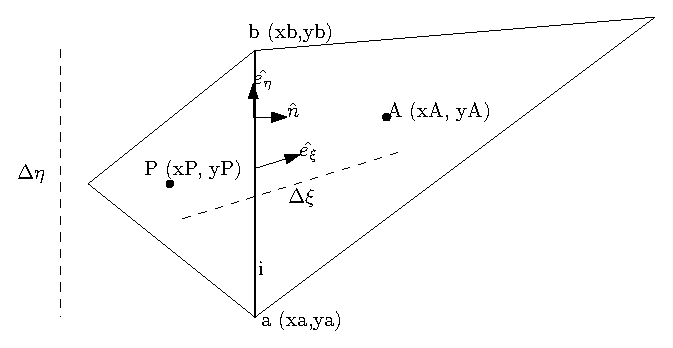
\includegraphics{fig/geometrias.eps}
    \caption{Geometrias para cálculos das expressões}
    \label{fig:geometrias}
\end{figure}

Na figura \ref{fig:geometrias}, P é o centroide do volume de controle para o qual a discretização é feita. O ponto A corresponde ao centroide do volume de controle vizinho e $\hat{e_\xi}$ é um vetor unitário (versor) na direção da linha que une os pontos P e A. A face i separa os dois volumes de controle e a-b é uma linha que une os pontos a e b, vértices compartilhados por ambos os volumes. As coordenadas dos pontos a e b são $(x_a, y_a)$ e $(x_b, y_b)$, respectivamente, enquanto $\hat{n}$ e $\hat{e_\eta}$ são, respectivamente, o vetor unitário normal (direcionado para fora do volume) e o vetor unitário tangente à face i.

Considerando-se a face i, apresentada na figura \ref{face-i} temos:

\begin{figure}[h]
    \centering
    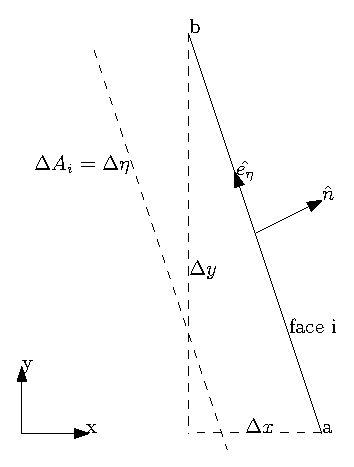
\includegraphics{fig/face-i.eps}
    \caption{Face i}
    \label{face-i}
\end{figure}

Tem-se que a área de tal face é calculada como:

\begin{equation}
    \label{eq:6.11}
    \Delta A_i = \sqrt{(\Delta x)^2 + (\Delta y)^2}
\end{equation}

Sendo:

\begin{equation}
    \label{eq:6.12}
    \Delta x = x_b - x_a
\end{equation}

\begin{equation}
    \label{eq:6.13}
    \Delta y = y_b - y_a
\end{equation}

O vetor unitário normal à superfície i é definida como:

\begin{equation}
    \label{eq:6.14}
    \hat{n} = \frac{\Delta y}{\Delta A_i}\hat{i} - \frac{\Delta x}{\Delta A_i}\hat{j}
\end{equation}

Na ausência de uma estrutura de malha, é necessário criar uma estrutura de dados para as informações geométricas, identificando a relação entre vértices, índices dos volumes, faces relevantes e volumes vizinhos (conectividades).

\section{Geração de malhas triangulares}

Malhas com elementos triangulares (ou tetraédricos) são malhas versáteis que podem preencher com facilidade domínios bastante irregulares, mas apresentam a dificuldade de ordenação que implica em matrizes de coeficientes sem a estrutura de bandas.

Como qualquer tipo de malha, malhas triangulares devem obedecer a certos requisitos, ou possuir certas propriedades, para que a solução numérica tenha qualidade. As propriedades de uma malha são definidas pelo número, forma e tamanho dos elementos, sendo o tempo de CPU e a memória utilizados para a geração também parâmetros importantes. Satisfazer os critérios de boa qualidade de malha e minimizar o tempo de processamento são processos contrários, pois melhorar a qualidade de uma malha significa, quase sempre, em aumentar o esforço computacional. Dessa contradição vem a dificuldade de criar-se geradores versáteis e rápidos e qu atendam aos requisitos numéricos.

Depois de bem representada através das superfícies, a fronteira de cálculo deve coincidir o melhor possível com a malha. Deste modo, tem-se que uma das mais importantes propriedades da malha é a sua coincidência com a fronteira, uma vez que disso depende a correta aplicação das condições de contorno. O controle do tamanho dos elementos é um parâmetro que é facilmente incluído em um gerador de malhas, o controle da forma dos elementos, contudo, é algo mais difícil de se conseguir.

Para uma malha que utilize elementos triangulares, é desejável que os mesmos sejam o mais próximo possível de triângulos equiláteros, pois isto permite que as funções de interpolação representem bem as variáveis dentro do triângulo. Quando um triângulo se afasta por demais do padrão equilátero, tem-se o equivalente a um elemento com elevada razão de aspecto em malhas com quadriláteros. Neste caso, observa-se uma elevada anisotropia nos coeficientes, o que reduz a taxa de convergência do processo de solução do sistema linear.

Além disso, é necessário que as dimensões do elemento variem de forma suave dentro do domínio e não de forma brusca, de modo a evitar volumes de controle irregulares, no qual o centroide se localiza próximo a duas faces do volume e, portante, não se configura em um ponto representativo de todo o volume de controle. É importante, assim, que a malha apresente certa uniformidade.

Outra propriedade de um gerador deve ser sua capacidade de adequação ao problema físico. Isto deve ser feito externamente ao gerador, pois é necessário que se conheça o comportamento da solução, de modo a se gerar a malha com refinamento em locais onde seja requerido. A forma automática de se executar essa tarefa, denominada adaptabilidade, é um ponto forte do gerador.

\begin{figure}[ht]
    \begin{subfigure}{.5\textwidth}
        \centering
        
\includegraphics[width=.8\linewidth]{fig/escaleno.eps}
        \caption{Elemento escaleno}
        \label{fig:sub-escaleno}
    \end{subfigure}
    \begin{subfigure}{.5\textwidth}
        \centering
        
\includegraphics[width=.4\linewidth]{fig/equilatero.eps}
        \caption{Elemento equilátero}
        \label{fig:sub-second}
    \end{subfigure}

    \begin{subfigure}{.5\textwidth}
        \centering
        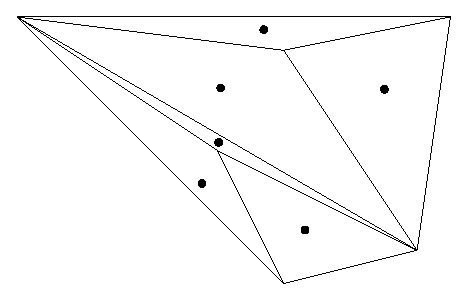
\includegraphics[width=.8\linewidth]{fig/variacao_brusca.eps}
        \caption{Variação brusca nas dimensões dos elementos}
        \label{fig:sub-brusca}
    \end{subfigure}
    \begin{subfigure}{.5\textwidth}
        \centering
        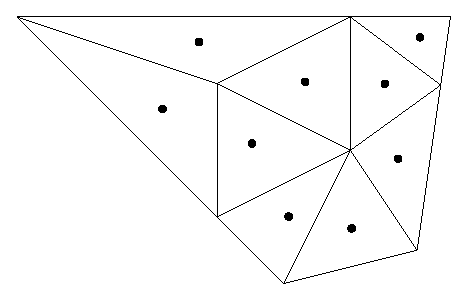
\includegraphics[width=.8\linewidth]{fig/variacao_suave.eps}
        \caption{Malha com variação mais suave dos elementos}
        \label{fig:sub-suave}
    \end{subfigure}
    \caption{Comparação de elementos desejáveis/indesejáveis}
    \label{fig:figlegal}
\end{figure}

\chapter[SUAVIZAÇÃO DE MALHAS NÃO ESTRUTURADAS]{SUAVIZAÇÃO DE MALHAS NÃO ESTRUTURADAS}

Embora ferramentas de geração de malhas automáticas sejam amplamente usadas, essas ferramentas podem não garantir a qualidade das malhas. Não apenas no processo de tesselação, mas também no refinamento da malha, é possível que alguns elementos severamente distorcidos ou fora de forma sejam criados. Mesmo quando uma malha uniforme é desejada, a ferramenta de tesselação pode gerar elementos que são muito pequenos ou muito grandes comparados com os elementos desejados. \cite{Zhou}

Existem vários tipos de esquemas de suavização de malhas, tais como suavização Laplaciana e suavização baseada em otimização. Tipicamente cada método possui um compromisso entre qualidade e custo computacional. Por exemplo, a suavização Laplaciana requer um custo computacional muito baixo, mas frequentemente resulta em uma malha de baixa qualidade nos elementos ou mesmo com elementos inválidos. Por outro lado, enquanto suavizações baseados na otimização são mais prováveis em evitar elementos inválidos e obtém uma maior qualidade na malha, o custo computacional é muito maior que a suavização Laplaciana. \cite{Zhou}

\section{Suavização Centroidal Voronoi Tessellation}

O método \textit{centroidal Voronoi tesselation} é uma tesselação cujos pontos gerados são os centróides das regiões de Voronoi correspondentes. \cite{Du1999}

Dado um conjunto aberto $\Omega \subset \mathbb{R}^N$, o conjunto ${V_i}_{i=1}^k$ é chamado de uma tesselação de $\Omega$ se $V_i \cap V_j = \emptyset$ para $i \neq j$ e $\cup_{i=1}^k \hat{V_i} = \hat{\Omega}$.

Dado um conjunto de pontos ${z_i}_{i=1}^k$ pertencentes a $\hat{\Omega}$, a região de Voronoi $\hat{V_i}$ que corresponde aos pontos $z_i$ é definida por:

\begin{equation}
    \hat{V_i} = {x \in \Omega |  |x-z_i| < |x-z_j| \text{para} j=1,...,j, j \neq i }
\end{equation}

Os pontos ${z_i}_{i=1}^k$ são chamados de sementes. Enquanto que o conjunto ${\hat{V_i}}_{i=1}^k$ é chamado de diagrama de Voronoi de $\Omega$ e cada $\hat{V_i}$ se refere a região de Voronoi correspondente a $z_i$.

Pode-se entender um diagrama de Voronoi como um conjunto de células em que as fronteiras dessas células estão de tal forma que os pontos contidos nas células são os mais próximos de um ponto específico. Ou seja, um diagrama de Voronoi é uma maneira de particionar um plano em regiões conhecidas como células baseado na distância de um conjunto específico de pontos conhecidos como sementes. Cada célula possui uma semente e os pontos nessa célula estão mais próximos dessa semente do que qualquer outra semente. Além disso pode-se considerar as regiões de Voronoi como poliedros.

Dado uma região $V \subset \mathbb{R}^N$ e uma função densidade $\rho$, definida em $V$, o centróide de massa $z^*$ de $V$ é definido como:

\begin{equation}
    z^* = \frac{\int_V y \rho(y) dy}{\int_V \rho(y) dy}
\end{equation}

Dado $k$ pontos $z_i$, $i=1,...,k$ podemos definir as suas regiões de Voronoi associadas $\hat{V_i},i=1,...,k$. Por outro lado, dados as regiões $\hat{V_i},i=1,...,k$ podemos definir seus centros de massa $z_i^k,i=1,...,k$. Nesse caso, interessa a situação em que:

\begin{equation}
    z_i = z_i^*, i=1,...,k
\end{equation}

Ou seja, os pontos $z_i$ que servem como as sementes (ou geradores) das regiões de Voronoi $\hat{V_i}$ são também os centros de massa dessas regiões. Chama-se tal tesselação como "centroidal Voronoi tessellation". A diferença entre uma tesselação de Voronoi e uma tesselação de Voronoi centrada pode ser visualizada na figura \ref{fig:voronoi_tessellation}.

\begin{figure}
    \centering
    
\includegraphics{fig/voronoi_tessellation.eps}
    \caption[Tesselação de Voronoi]{Tesselação de Voronoi}
    \label{fig:voronoi_tessellation}
\end{figure}

% \subsubsection{Fixed Point Uniform}

% O primeiro método de suavização de malha é chamado de Fixed Point Uniform e consiste em mover as sementes das células para o valor da média ponderada dos centroides das células vizinhas. Com essas novas sementes se refaz a tesselação de Voronoi e ligando-se os centroides das novas células, tem-se as triangulações de Delaunay.

\section{Suavização de Laplace}

A suavização de Laplace é o método mais comum e direto para suavisar uma malha. Ele apenas move cada nó para o centróide do polígono formado pelos nós adjacentes. Ele é um algoritmo de suavização local porque, em cada passo, o movimento do nó é calculado usando-se a localização dos seus nós adjacentes apenasa. Normalmente realiza-se a iteração apenas algumas vezes porque a qualidade da malha não é melhorada com novas iterações; de fato a qualidade pode, muitas vezes, piorar. \cite{Zhou}

Na suavização de Laplace nós podemos considerar a malha como um sistema de molas como mostrado na figura \ref{fig:laplacian_smoothing}. Cada aresta conectando ao nó central com os seus nós vizinhos podem ser vistos como um sistema linear de molas com um tamanho inicial de zero. Seja $\vec{v_i}$ o vetor do nó central com o i-ésimo nó vizinho:

\begin{equation*}
    \vec{v_i} = (x_i - x, y_i - y)
\end{equation*}

A soma das forças de mola agindo no nó central é:

\begin{equation*}
    \vec{F} = K \sum_{i=1}^k \vec{v_i}
\end{equation*}

Em que $K$ é a constante de mola, e $k$ é o número de nós vizinhos. Quando o nó central é localizado exatamente no centro geométrico do polígono, as forças de mola estão balanceadas e o sistema de mola está em equilíbrio.

Enquanto a suavização de Laplace é uma maneira iterativa de se achar este estado de forças balanceadas, nós podemos também resolver esse problema por minimização de energia do sistema de molas. Considerando que todas as molas tem um comprimento inicial de zero, nós podemos computar a energia potencial do sistema como:

\begin{equation*}
    E = \sum_{i=1}^k \frac{1}{2} K (||\vec{v_i}||)^2
\end{equation*}

Este é um problema de otimização, em que a função de custo é esta função quadrática. Minimizando-se esta função de custo nós podemos obter o mesmo resultado de se usar a suavização de Laplace.


A suavização de Laplace pode, portanto, ser vista como um tipo de otimização nodal local. A função de custo é a soma dos mínimos quadrados dos comprimentos das arestas compartilhadas pelo mesmo nó:

\begin{equation*}
    f(x,y) = \sum_{i=1}^k ((x-x_i)^2 + (y-y_i)^2)
\end{equation*}

Devido ao custo da função de suavização de Laplace ser o de uma função quadrática, ela se torna muito simples de achar a posição do nó que irá minimizar essa função. Podemos obter a posição $(x,y)$ que minimiza a função de custo simplesmente encontrando-se o centro geométrico dos nós vizinhos:

\begin{equation*}
    \frac{\partial f}{\partial x} = \frac{\partial f}{\partial y} = 0
\end{equation*}

\begin{equation*}
    x = \frac{1}{k} \sum_{i=1}^k x_i, y = \frac{1}{k} \sum_{i=1}^k y_i
\end{equation*}

Essa função de curso, no entaanto, não reflete necessariamente a qualidade da malha, e essa é a razão pela qual a suavização de Laplace frequentemente falha em melhorar a qualidade da malha, e em alguns casos, até mesmo gera elementos inválidos.

Abaixo está listado as vantagens e desvantagens da suavização de Laplace:

Vantagens:
\begin{itemize}
    \item Computacionalmente eficiente
    \item Fácil de ser implementada
\end{itemize}

Desvantagens:
\begin{itemize}
    \item Nem sempre move o nó para a posição ótima de modo a se obter o elemento de melhor qualidade
    \item Pode gerar elementos invertidos
    \item Tende a perder a uniformidade de tamanho caso a iteração rode mais que algumas vezes
    \item Tende a gerar elementos de menor qualidade caso a iteração rode mais que algumas vezes
\end{itemize}

\section{Suavização baseada em otimização}

Métodos baseados em suavização por otimização usam algumas medidas de qualidade da malha de modo a definir as funções de custo. Os nós da malha são movidos de modo a minimizar ou a maximizar essas funções.

Algumas funções de custo usadas nesse tipo de suavização são:

\begin{itemize}
    \item Mínimo/Máximo ângulo:\\
    O mínimo/máximo ângulo é um índice direto para se medir a qualidade da malha. Um elemento com ângulos próximos a 0º ou 180º irá criar dificuldades no processo de análise de elementos finitos. Na suavização baseada em otimização, portanto, ou o menor angulo é maximizado ou o maior angulo é minimizado de modo a se eliminar elementos severamente distorcidos.
    \item Razão de proporção:\\
    A razão de proporção é a razão entre o raio do círculo circunscrito com o círculo inscrito do elemento de malha. Um triângulo equilateral tem uma razão de proporção de 2.0. Quando um elemento se torna muito distorcido, a razão de proporção aumenta.
    \item Métricas de distorção:\\
    As métricas de distorção estão relacionadas com a área e com o comprimento das fronteiras dos elementos. A qualidade do formato de um elemento pode ser verificado quantitativamente usando-se este tipo de métricas. Um triângulo equilateral tem o melhor valor possível, e um elemento muito distorcido tem um valor próximo a zero. Essas métricas podem também ser usadas em elementos quadrilaterais.
\end{itemize}

Uma das vantagens de suavizações baseadas em otimização é a que elas garantem uma melhora na qualidade da malha. Otimizando a qualidade das medidas, elementos severamente distorcidos são efetivamente elimidados. O custo computacional, no entanto, é muito maior do que a suavização de laplace. Para um elemento triangulos 2D, por exemplo, a suavização baseada em otimização pode ser cinco vezes mais caro computacionalmente que a suavização de Laplace esperta \cite{Freitag1997OnCL}, e 30 a 40 vezes mair caro computacionalmente que a suavização de Laplace.

\section{Suavização baseada na otimização de ângulos}

Segundo \cite{Zhou}, o método de suavização de malhas 2D baseado em ângulos compara cada nó da malha com os pares de ângulos adjacentes incidentes no nó e ajusta-se esses ângulos de modo que eles se tornam iguais no caso de uma malha triangular. No artigo é mostrado que essa técnica de suavização gera uma malha de maior qualidade em relação ao método da suavização Laplaciana e com um menor custo computacional.

\subsection{Algoritmo}
Esta seção descreve o algoritmo de suavização baseado em ângulos para uma malha triangular. A ideia central desse método é fazer com que cada par de ângulos adjacentes sejam iguais ou em uma certa razão, isso é eficaz para eliminar ângulos próximos a 0º ou 180º. Este método é fácil de ser implementado, e a qualidade da malha resultante é significativamente melhor que aplicando-se a suavização de Laplace, enquanto que o custo computacional é muito menor que as suavizações baseadas em otimização.

Nesse algoritmo, pode-se fazer uma analogia com um sistema de molas. A diferença entre este método e o método Laplaciano é que as molas usadas aqui são molas de torção. A energia potencial de tal sistema de molas de torção é:

\begin{equation*}
    E = \sum_{i=1}^{2k} \frac{1}{2} K \Theta_i^2
\end{equation*}

onde $k$ é o número de vértices do polígono, $K$ é a constante de mola e $\Theta$ é o ângulo na fronteira do polígono. Cada par de ângulos compartilha um vértice do polígono, portanto, existem $2k$ ângulos no total para serem considerados.

\begin{figure}[h]
    \centering
    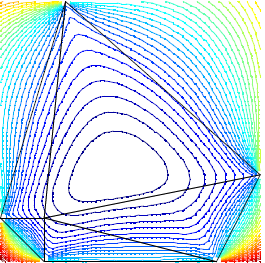
\includegraphics{fig/contorno-mola-torcao.png}
    \caption{Energia do sistema de molas de torção}
    \label{fig:contorno-mola-torcao}
\end{figure}

A plotagem do contorno dessa energia é mostrada na figura \ref{fig:contorno-mola-torcao}. É usado o mesmo polígono que a suavização de Laplace. Comparando-se essas duas plotagens, nós encontramos que a posição de energia mínima é diferente nos dois casos. A suavização baseada em ângulos fornece uma melhor localização em relação ao método de Laplace.

É implementado um método iterativo que irá minimizar a energia potencial do sistema de molas de torção. O algoritmo de suavização baseado em ângulos é resumido nos seguintes cinco passos:

\begin{enumerate}
    \item Como mostrado na figura \ref{fig:angle-based}, para cada nó $N_i$, existem $k$ pares de ângulos ao redor dele, onde $k$ é o número de nós vizinhos. Os dois ângulos adjacentes são calculados como:
    
    \begin{equation*}
        \alpha_1 = \arccos{\qty(\frac{\vec{v_j} \cdot \vec{v_{j+1}}}{\norm{\vec{v_j}} \norm{\vec{v_{j+1}}} })}
    \end{equation*}
    \begin{equation*}
        \alpha_2 = \arccos{\qty(\frac{\vec{v_j} \cdot \vec{v_{j-1}}}{\norm{\vec{v_j}} \norm{\vec{v_{j-1}}} })}
    \end{equation*}

    Onde $\vec{v_{v-i}}$, $\vec{v_j}$ e $\vec{v_{j+1}}$ são vetores que compartilham o vértice $N_j$; $\norm{\vec{v}}$ é a norma $L_2$ do vetor; e $\alpha_1$, $\alpha_2$ são os ângulos determinados pelos três vetores.

    \begin{figure}[]
        \centering
        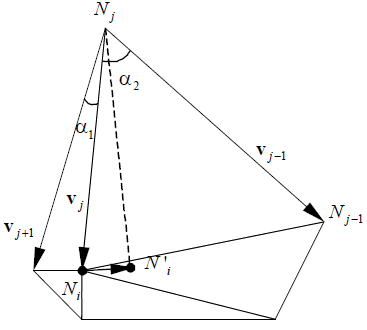
\includegraphics{fig/angle-based.png}
        \caption{Método de suavização baseado em ângulos}
        \label{fig:angle-based}
    \end{figure}

    \item Calcular a diferença entre dois ângulos adjacentes, e decidir qual o ângulo que o vetor $\vec{v_j}$ será rotacionado:
    
    \begin{equation*}
        \beta_j = (\alpha_2 - \alpha_1) / 2
    \end{equation*}

    Onde $\beta_j$ é o ângulo pelo qual o vetor $\vec{v_j}$ irá rotacionar.

    \item Rotacional o vetor $\vec{v_j}$ no ângulo $\beta_j$ ao redor de $N_j$, de modo que as novas coordenadas do nó $N_i$ serão:
    
    \begin{equation*}
    \begin{split}
        x' = x_0 + (x-x_0) \cos{\beta_j} - (y-y_0) \sin{\beta_j}\\
        y' = y_0 + (x-x_0) \sin{\beta_j} + (y-y_0) \cos{\beta_j}
    \end{split}
    \end{equation*}

    Onde $(x_0, y_0)$ é a localização do nó $N_j$, $(x,y)$ é a localização antiga do nó $N_i$ e $(x', y')$ é a nova localização do nó $N_i$.

    \item Iterando-se todos os nós vizinhos, existem $k$ conjuntos de novas localizações para o mesmo nó $N_i$. É computado agora a localização final do nó $N_i$ pegando-se a média de $(x', y')$ computada de todos os nós vizinhos.
    
    \begin{equation*}
    \begin{split}
        x_{new} = \frac{1}{k} \sum_{i=1}^k x'_i\\
        y_{new} = \frac{1}{k} \sum_{i=1}^k y'_i
    \end{split}
    \end{equation*}
\end{enumerate}


\chapter[DIFUSÃO DE CALOR 2D EM REGIME PERMANENTE]{DIFUSÃO DE CALOR 2D EM REGIME PERMANENTE}

\label{dif2d}

Para o estudo da difusão de calor 2D em regime permanente, parte-se das seguintes hipóteses:
\begin{itemize}
    \item Difusão de calor 2D
    \item Regime permanente
    \item Propriedades termofísicas constantes
    \item Presença de termo fonte
\end{itemize}

Sob esses hipóteses, tem-se a seguinte equação governante:

\begin{equation}
    \label{eq:8.1}
    \frac{\partial^2 T}{\partial x^2} + \frac{\partial^2 T}{\partial y^2} = S^\phi
\end{equation}

Que pode ser reescrita como:

\begin{equation}
    \label{eq:8.2}
    \vec{\nabla} \cdot (\vec{\nabla} T) = S^\phi
\end{equation}

Tal expressão deve ser, então, integrada para cada volume de controle do domínio discretizado, de modo que:

\begin{equation}
    \label{eq:8.3}
    \int_{vc} \vec{\nabla} \cdot (\vec{\nabla}T) dv = \int_{vc}S^\phi dv
\end{equation}

Aplicando-se, na sequência, o teorema da divergência de Gauss no lado esquerdo da equação anterior, tem-se:

\begin{equation}
    \label{eq:8.4}
    \int_A \hat{n} \cdot (\vec{\nabla T}) dA = \int_{vc} S^\phi dv
\end{equation}

Ou seja,

\begin{equation}
    \label{eq:8.5}
    \sum_{superficies} \int_{\nabla A_i} \hat{n} \cdot (\vec{\Delta}T)dA = \int_{vc} S^\phi dv
\end{equation}

A integração de superfície de cada elemento é aproximada pelo produto interno entre o vetor normal (direcionado para fora do volume de controle) à superfície $\hat{n_i}$ e um vetor de fluxo difusivo $(\vec{\Delta}T)$ que atravessa a superfície do elemento de controle $(\Delta A_i)$. O primeiro termo da equação \ref{eq:8.5} pode ser aproximado empregando-se o método de diferenças centrais ao longo da linha $PA$. Deste modo,

\begin{equation}
    \label{eq:8.6}
    \int_{\Delta A_i} \hat{n_i} \cdot (\vec{\nabla}T)dA \approx \hat{n_i} \cdot (\vec{\nabla}T) \Delta A_i \approx \frac{T_A - T_P}{\Delta \xi} \Delta A_i
\end{equation}

\begin{figure}[ht]
    \begin{subfigure}{.5\textwidth}
        \centering
        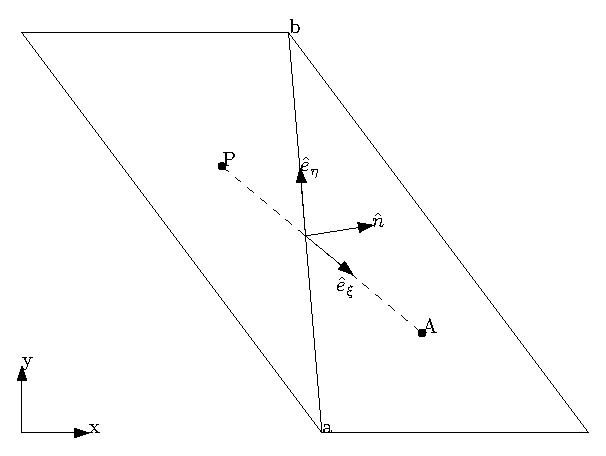
\includegraphics[width=.8\linewidth]{fig/difusao-cruzada-a.eps}
        \caption{}
        \label{fig:8.1-a}
    \end{subfigure}
    \begin{subfigure}{.5\textwidth}
        \centering
        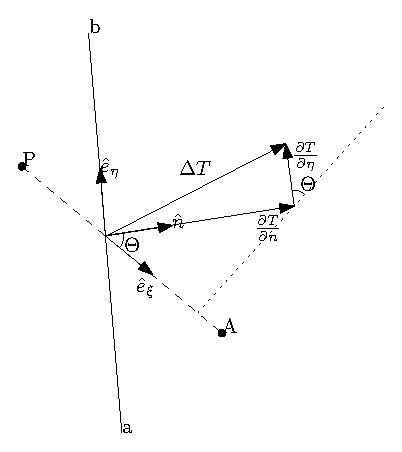
\includegraphics[width=.8\linewidth]{fig/difusao-cruzada-b.eps}
        \caption{}
        \label{fig:8.1-b}
    \end{subfigure}

    \begin{subfigure}{.5\textwidth}
        \centering
        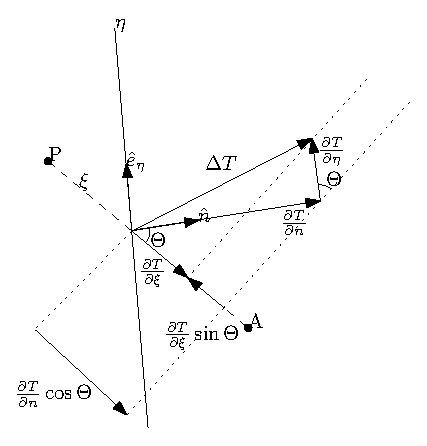
\includegraphics[width=.8\linewidth]{fig/difusao-cruzada-c.eps}
        \caption{}
        \label{fig:8.1-c}
    \end{subfigure}

    \caption{Esquemas para definição do termo de difusão cruzada}
    \label{fig:8.1}
\end{figure}

Na equação \ref{eq:8.6} $\Delta \xi$ é a distância entre os centroides A e P. Nota-se que a diferença central na equação \ref{eq:8.6} só é acurada se a linha que une os pontos A e P e o vetor normal unitário $\hat{n_i}$ estão na mesma direção, ou seja, a aproximação só é correta no caso em que a malha é completamente ortogonal. Normalmente, em malhas não-estruturadas as linhas que conectam os centroides P e A não são paralelas ao vetor normal unitário $\hat{n_i}$. Isto é conhecido como não-ortogonalidade de malha (mesh skewness ou mesh non-orthogonality). O cálculo do fluxo na equação \ref{eq:8.6} deve, desse modo, ser corrigido pela adição de uma contribuição provocada pela não-ortogonalidade. Existem diversos meios de realizar essa correção, mas a forma mais comum é a de introduzir um termo conhecido como difusão cruzada (cross diffusion), que é tratada como termo-fonte na equação discretizada.

Seguindo-se a metodologia proposta por Mathur e Murthy (1997), tem-se que o termo de difusão cruzada é obtido, introduzindo-se as coordenadas $\xi$ e $\eta$, sendo: $\xi$ definida ao longo da linha que une os pontos A e P, e $\eta$ ao longo da face do volume de controle (ao longo da linha que une os vértices a e b). Desse modo, o gradiente $\vec{\Delta}T$ pode ser expresso por:

\begin{equation}
    \label{eq:8.7}
    \vec{\nabla}T = \frac{\partial T}{\partial x}\hat{i} + \frac{\partial T}{\partial y}\hat{j} = \frac{\partial T}{\partial n}\hat{n} + \frac{\partial T}{\partial \eta}\hat{e_\eta}
\end{equation}

Sendo $\hat{i}$ e $\hat{j}$ vetores unitários nas direções $x$ e $y$ e $\hat{n}$ e $\hat{e_\eta}$ vetores unitários ao longo das direções normal e tangencial.

O vetor unitário normal $\hat{n}$, bem como os vetores unitários nas direções $\xi$ e $\eta$, $\hat{e_\xi}$ e $\hat{e_\eta}$, respectivamente, podem ser expressas através das seguintes relações envolvendo centroides e vértices:

\begin{equation}
    \label{eq:8.8}
    \hat{n} = \frac{\Delta y}{\Delta A_i}\hat{i} - \frac{\Delta x}{\Delta A_i}\hat{j} = \frac{y_b - y_a}{\Delta \eta}\hat{i} - \frac{x_b - x_a}{\Delta \eta}\hat{j}
\end{equation}

\begin{equation}
    \label{eq:8.9}
    \hat{e_\xi} = \frac{x_A - x_P}{\Delta \xi}\hat{i} + \frac{y_A - y_P}{\Delta \xi}\hat{j}
\end{equation}

\begin{equation}
    \label{eq:8.10}
    \hat{e_\eta} = \frac{x_b - x_a}{\Delta \eta}\hat{i} + \frac{y_b - y_a}{\Delta \eta}\hat{j}
\end{equation}

Uma observação que deve ser feita a respeito da equação \ref{eq:8.6} é a que ela é uma aproximação real de $\partial T/\partial \xi$ apenas no caso de uma malha ortogonal, ou seja, quando $\partial T/\partial \xi = \partial T/\partial n$. Caso contrário, para malhas não-ortogonais, $\partial T/\partial \xi$ pode ser muito diferente de $\partial T/\partial n$.

Observa-se nas figuras \ref{fig:8.1-b} e \ref{fig:8.1-c} que $\partial T/\partial \xi$ corresponde ao comprimento da projeção do vetor $\vec{\Delta}T$ na direção de $\xi$. Empregando a equação \ref{eq:8.7}, pode-se representar também $\vec{\Delta}T$ como a soma de $(\partial T/\partial n)\hat{n}$ e $(\partial T/\partial \eta)\hat{e_\eta}$, conforme a figura \ref{fig:8.1-c}.

Para se obter uma melhor estimativa do fluxo normal $\hat{n} \cdot \vec{\Delta}T = \partial T/\partial n$, examina-se a relação entre a projeção de $\vec{\Delta}T$ na direção $\xi$ que é $(\partial T/\partial \xi)$ e as projeções nessa direção de duas componentes de $\vec{\Delta}T$ que são: $(\partial T/\partial n)\hat{n} \cdot \hat{e_\xi}$ e $(\partial T/\partial \eta)\hat{e_\eta} \cdot \hat{e_\xi}$.

Denotando-se o ângulo entre as direções $\hat{n}$ e $\xi$ por $\Theta$, tem-se que:

\begin{equation}
    \label{eq:8.11}
    \frac{\partial T}{\partial n} \hat{n} \cdot \hat{e_\xi} = \frac{\partial T}{\partial n} \cos{\Theta}
\end{equation}

e

\begin{equation}
    \label{eq:8.12}
    \frac{\partial T}{\partial \eta} \hat{e_\eta} \cdot \hat{e_\xi} = - \frac{\partial T}{\partial \eta} \sin{\Theta}
\end{equation}

Deste modo, tem-se que:

\begin{equation}
    \label{eq:8.13}
    \frac{\partial T}{\partial \xi} = \frac{\partial T}{\partial n}\cos{\Theta} - \frac{\partial T}{\partial \eta} \sin{\Theta}
\end{equation}

Recorda-se, então, que $\hat{n} \cdot \vec{\Delta}T = \partial T/\partial n$ e, rearranjando os termos da equação \ref{eq:8.13}, obtém-se o fluxo difusivo da equação \ref{eq:8.6}:

\begin{equation}
    \label{eq:8.14}
    \hat{n} \cdot \vec{\Delta}T = \frac{\partial T}{\partial n} = \frac{\partial T}{\partial \xi} \frac{1}{\cos{\Theta}} + \frac{\partial T}{\partial \eta} \tan{\Theta}
\end{equation}

Os dois gradientes que transportam T no lado direito da equação \ref{eq:8.14} podem ser aproximados por diferenças centrais (CDS):

\begin{equation}
    \label{eq:8.15}
    \frac{\partial T}{\partial \xi} = \frac{T_A - T_P}{\Delta \xi}
\end{equation}

\begin{equation}
    \label{eq:8.16}
    \frac{\partial T}{\partial \eta} = \frac{T_b - T_a}{\Delta \eta}
\end{equation}

Onde $\Delta \xi$ é a distância entre os centroides $A$ e $P_i$ e $\Delta \eta$ é a distância entre os vértices $a$ e $b$ ($\Delta \eta = \Delta A_i)$.

Na literatura, tem-se que $\partial T/\partial \xi$ e $\partial T/\partial \eta$ são chamaods de gradiente direto (Direct Gradient) e difusão cruzada (Cross Diffusion), respectivamente. A substituição das aproximações por diferenças centrais, equações \ref{eq:8.15} e \ref{eq:8.16} na equação \ref{eq:8.14} resulta em:

\begin{equation}
    \label{eq:8.17}
    \hat{n} \cdot \vec{\nabla}T \Delta A_i = \frac{\Delta A_i}{\cos{\Theta}} \frac{T_A - T_P}{\Delta \xi} + \Delta A_i \tan{\Theta} \frac{T_b - T_a}{\Delta \eta}
\end{equation}

Da figura \ref{fig:8.1}, observa-se que:

\begin{equation}
    \label{eq:8.18}
    \frac{1}{\cos \Theta} = \frac{1}{\hat{n}\cdot \hat{e_\xi}} = \frac{\hat{n} \cdot \hat{n}}{\hat{n} \cdot \hat{e_\xi}}
\end{equation}

e

\begin{equation}
    \label{eq:8.19}
    \tan{\Theta} = \frac{\sin{\Theta}}{\cos{\Theta}} = - \frac{\hat{e_\xi} \cdot \hat{e_\eta}}{\hat{n} \cdot \hat{e_\xi}}
\end{equation}

Lembrando-se que:

\begin{equation}
    \label{eq:8.20}
    \vec{a} \cdot \vec{b} = |a| |b| \cos{\Theta}
\end{equation}

e

\begin{equation}
    \label{eq:8.21}
    \cos{\pi / 2 = \alpha} = - \sin{\alpha}
\end{equation}

Deste modo, a equação \ref{eq:8.17} pode ser escrita na forma vetorial como:

\begin{equation}
    \label{eq:8.22}
    \hat{n} \cdot \vec{\nabla} T \Delta A_i = \frac{\hat{n} \cdot \hat{n} \Delta A_i}{\hat{n} \cdot \hat{e_\xi}} \frac{T_A - T_P}{\Delta \xi} - \frac{\hat{e_\xi} \cdot \hat{e_\eta} \Delta A_i}{\hat{n} \cdot \hat{e_\xi}} \frac{T_b - T_a}{\Delta \eta}
\end{equation}

Os fatores $\hat{n} \cdot \hat{n} \Delta A_i / (\hat{n} \cdot \hat{e_\xi})$ e $\hat{e_\xi} \cdot \hat{e_\eta} \Delta A_i / (\hat{n} \cdot \hat{e_\xi})$ podem ser obtidos da geometria dos elementos de malha.

Normalmente, o termo de disufão cruzada é tratado como termo-fonte na equação dicretizada. Deste modo, separando-se o termo de difusão cruzada da equação \ref{eq:8.22}, obtém-se:

\begin{equation}
    \label{eq:8.23}
    \hat{n} \cdot \vec{\nabla}T \Delta A_i = \frac{\hat{n} \cdot \hat{n} \Delta A_i}{\hat{n} \cdot \hat{e_\xi}} \frac{T_A - T_P}{\Delta \xi} + S_{DC}
\end{equation}

Para a estimativa do termo de difusão cruzada, é necessário avaliar o $\vec{\nabla}T$ ao longo da linha $ab$. Existem vários métodos que podem ser empregados nesse cáclulo. Um deles consiste em interpolar os valores de $T$ nodais (obtidas para os centroides) para calcular os valores de $T_a$ e $T_b$ e então estimar o gradiente. Empregando-se a média entre todos os pontos nodais vizinhos ao vértice $a$ conduz a:

\begin{equation}
    \label{eq:8.24}
    T_a = \frac{T_P + T_A + T_B + \dots}{N}
\end{equation}

Onde $N$ é o número total de nós (centroides) ao redor do vértice $a$. Uma alternativa é empregar uma média ponderada pela distância entre o vértice e os nós, cujo resultado é mais acurado, porém, também mais caro computacionalmente.

O termo-fonte, da equação \ref{eq:8.15}, é tratado de modo semelhante ao método empregado para malhas ortogonais, ou seja:

\begin{equation}
    \label{eq:8.25}
    \int_{vc} S^\phi dv = \bar{S} \Delta v
\end{equation}

Onde $\Delta v$ é o volume do volume de controle envolvido, e $\bar{S}$ é o valor médio de $S^\phi$ sobre todo o volume de controle.

A aproximação da equação \ref{eq:8.25}, com uma aproximação de segunda ordem de acurácia, é obtida ao se empregar o teorema do valor intermediário para integrais, substituindo-se o valor médio $\bar{S}$ pelo valor nodal da função $S$ aplicado no centroide do volume de controle. No caso bidimensional, o volume $\Delta v$ corresponde à área do elemento de malha multiplicada por um comprimento unitário na direção normal ao plano bidimensional. Assim:

\begin{equation}
    \label{eq:8.26}
    \int_{vc} S^\phi dv = S_P \Delta v
\end{equation}

No caso 2D tem-se que $\Delta v = \Delta A$.

Antes de efetuar o acoplamento das diversas partes da equação discretizada para se obter o sistema de equações lineares correspondente. A equação \ref{eq:8.23} será reescrita como:

\begin{equation}
    \label{8.27}
    \hat{n} \cdot \vec{\nabla}T \Delta A_i = D_i (T_A-T_P) + S_{DC,i}
\end{equation}

Onde

\begin{equation}
    \label{eq:8.28}
    D_i = \frac{\hat{n_i} \cdot \hat{n_i}}{\hat{n_i} \cdot \hat{e_{\xi,i}}} \frac{\Delta A_i}{\Delta \xi}
\end{equation}

e

\begin{equation}
    \label{eq:8.29}
    S_{DC,i} = - \frac{\hat{e_{\xi,i}} \cdot \hat{e_{\eta,i}}}{\hat{n_i} \cdot \hat{e_{\xi,i}}} \frac{\Delta A_i}{\Delta \eta_i} (\phi_b - \phi_a)
\end{equation}

Generalizando-se a equação \ref{8.27} para todas as faces de um volume de controle e utilizando-se também a equação \ref{eq:8.26} na equação \ref{eq:8.25}, obtém-se:

\begin{equation}
    \label{eq:8.30}
    \sum_{i=1}^{nb} [ D_i (T_i - T_P) + S_{DC,i}] = S_P \Delta v
\end{equation}

No caso 2D tem-se que $\Delta v = \Delta A$ e onde:

\begin{equation}
    \label{eq:8.31}
    D_i = \frac{\hat{n_i} \cdot \hat{n_i}}{\hat{n_i} \cdot \hat{e_{\xi,i}}} \frac{\Delta A_i}{\Delta \xi}
\end{equation}

\begin{equation}
    \label{eq:8.32}
    S_{DC,i} = - \frac{\hat{e_{\xi,i}} \cdot \hat{e_{\eta,i}}}{\hat{n_i} \cdot \hat{e_{\xi,i}}} \frac{\Delta A_i}{\Delta \eta_i} (T_b - T_a)
\end{equation}

Sendo:

\begin{itemize}
    \item i: o índice referente a uma face qualquer do volume de controle
    \item nb: a quantidade total de faces do volume de controle
    \item P: o índice do centroide do volume de controle considerado
    \item Ti: a temperatura no centroide do volume de controle vizinho ao volume P, com compartilhamento da face i
    \item $\hat{n_i}$: o vetor normal unitário à face i, que aponta para fora do volume P
    \item $\hat{e_{\xi,i}}$: vetor unitário na direção $\xi$, para a face i
    \item $\hat{e_{\eta,i}}$: vetor unitário na direção $\eta$, para a face i
    \item $\xi$: direção da linha que une os centroides do volume P e do volume vizinho com compartilhamento da face i
    \item $\eta$: direção da linha que une os vértices a e b, pertencentes à face i
    \item $\Delta A_i$: área da face i, no caso 2D, $\Delta A_i = \Delta \eta$
    \item $\Delta v$: volume total do volume de controle P, no caso 2D, $\Delta v = \Delta A$ (área do elemento de malha).
    \item $T_b, T_a$: temperaturas avaliadas nos vértices $b$ e $a$, respectivamente, da face i (é conveniente que $b$ e $a$ estejam dispostos de tal modo que a ordenação dos vértices esteja no sentido anti-horário)
\end{itemize}

A equação \ref{eq:8.30} pode ser rearranjada para a forma:

\begin{equation}
    \label{eq:8.33}
    a_P T_P = \sum a_{nb} T_{nb} + b_P
\end{equation}

Sendo:

\begin{equation}
    \label{eq:8.34}
    a_P = \sum a_{nb}
\end{equation}

\begin{equation}
    \label{eq:8.35}
    \sum a_{nb} = \sum_{i=1}^{nb} S_{DC,i}
\end{equation}

\begin{equation}
    \label{eq:8.36}
    b_P = -S_P \Delta v = \sum_{i=1}^{nb} S_{DC,i}
\end{equation}

O sistema de equações, na forma da equação \ref{eq:8.33}, pode ser resolvido por qualquer método para solução de sistemas lineares. Caso o método escolhido seja o de Gauss-Seidel, tem-se que:

\begin{equation}
    \label{eq:8.37}
    T_P = (\sum a_{nb}T_{nb}+b_P)/a_P
\end{equation}

\section{Algoritmo}

O algoritmo apresenta os seguintes passos:

\begin{enumerate}
    \item Gerar a malha: tipos de elementos, vértices, centroides, conectividades
    \item Para um volume de controle P, calcular os coeficientes $a_P$ e $\sum a_{nb}$. Para tanto, é necessário.
    \begin{enumerate}
        \item Em cada face i, definem-se os vetores unitários: normal à superfície $(\hat{n})$, na direção da linha que une os vértices $a$ e $b$ da face $(\hat{e_\eta})$, e na direção da linha que une o centroide de P e o centroide do volume que compartilha a face i $(\hat{e_\xi})$: equações \ref{eq:8.8} a \ref{eq:8.10}, no caso 2D.
        \item Obter o valor de $D_i$, referente à face i, pela equação \ref{eq:8.28}
        \item Voltar ao passo 2a, para que sejam obtidos todos os vetores unitários $(\hat{n}, \hat{e_\xi}, \hat{e_\eta})$, bem como todos os valores de $D_i$ para as $nb$ faces do volume de controle, obtendo-se então todos os coeficientes $a_{nb}$.
    \end{enumerate}
    \item Calcular o termo-fonte $b_P$. Para tanto, é necessário calcular $\Delta v$ para o volume de controle P (no caso 2D, $\Delta v = \Delta A$). É necessário, também, avaliar a função $S^\phi$ no centroide do volume P, bem como calcular $S_{DC,i}$ para todas as $nb$ faces do volume P. Para o cálculo das temperaturas nos vértices, pode-se empregar a equação \ref{eq:8.24}, utilizando-se todos os centroides cujos volumes são construídos empregando-se o vértice em questão.
    \item Retornar ao passo 2, até que todos os volumes de controle da malha sejam avaliados.
    \item Resolver o sistema linear obtido através de um método como o de Gauss-Seidel, equação \ref{eq:8.37}
    \item Recalcular os termos-fontes de todos os volumes (Passo 3).
    \item Voltar ao passo 5 até que um dado critério de parada (Tolerância, número de iterações) seja atingido.
\end{enumerate}

\section{Condições de contorno}
A aplicação das condições de contorno pode ser realizada com o auxílio, por exemplo, de volumes fictícios. Neste caso, duas possibilidades são listadas:

\subsection{Volume espelhado}

Também chamado de volume simétrico, neste caso, apesar do vetor normal à superfície de controle que separa os volumes A e P ser paralelo à linha que une A a P, nota-se que há um desalinhamento entre o ponto médio da face (m) e a linha $\bar{AP}$. Neste caso, existe um erro de discretização relacionado ao fato de a linha $\bar{PA}$ não interceptar o ponto médio $m$ da face $ab$. Esse erro cresce com o aumento da não-ortogonalidade da malha, bem como com o aumento da razão de aspecto da malha como pode ser visto na figura \ref{contorno-1}.

\begin{figure}[h]
    \centering
    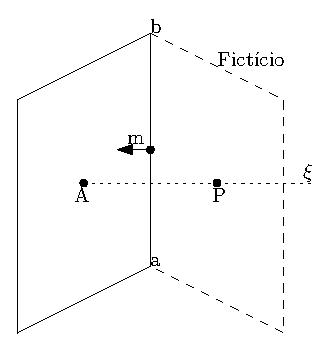
\includegraphics{fig/contorno-1.eps}
    \caption{Volume Espelhado}
    \label{contorno-1}
\end{figure}

Outro modo de se aplicar as condições de contorno com volumes fictícios é feita empregando-se um volume antissimétrico, ou seja, ele deve ser espelhado em ambas as direções (e e y), como se segue:

\subsection{Volume antissimétrico}

\begin{figure}[]
    \centering
    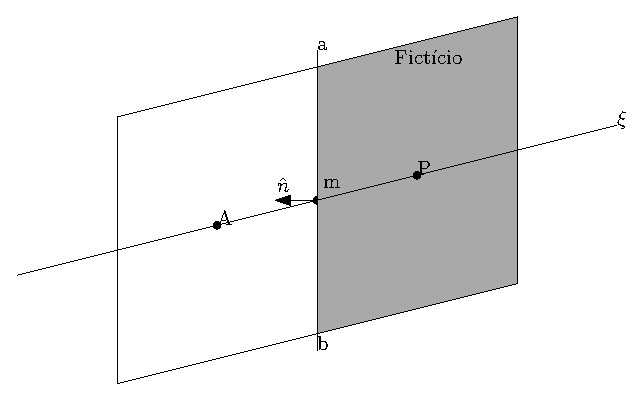
\includegraphics{fig/contorno-2.eps}
    \caption{Volume Antissimétrico}
    \label{contorno-2}
\end{figure}

Neste caso, a linha que une P e A passa pelo ponto médio da face $(m)$. Assim, não há o erro de não-ortogonalidade existente ao se aplicar o volume fictício espelhado (simétrico). Nota-se, contudo, que será necessário avaliar o termo de difusão cruzada, uma vez que o vetor normal $\hat{n}$ e o vetor unitário na direção $\xi$ podem não ser coincidentes. Nesse caso, será necessário empregar uma expressão semelhante à equação \ref{8.27}. Contudo, a temperatura nos vértices $T_a$ e $T_b$ pode ser avaliada mediante o uso das condições de contorno.

Uma importante observação a respeito da utilização de diferenças centrais envolvidas na integração da superfície dos elementos de controle diz respeito ao fato que sua acurácia será de segunda ordem apenas no caso em que as mesmas sejam avaliadas no ponto médio de $\hat{n} \cdot \vec{\nabla}T \Delta A_i$. Este não é o caso se as linhas PA e ab não se interceptam no ponto médio m de ab quando a malha é não-ortogonal.

Este erro aumenta com a não-ortogonalidade e a razão de aspecto da malha, de modo que um grande esforço deve ser feito com relação ao controle da não-ortogonalidade e da razão de aspecto em malhas não-estruturadas.

\chapter[ALGORÍTMO GENÉTICO]{ALGORÍTMO GENÉTICO}

Algoritmos Genéticos (GAs) são métodos adaptativos que podem ser usados para resolver problemas envolvendo procura e otimização. Eles são baseados nos processos genéticos de organismos biológicos. Ao longo de muitas gerações, populações naturais evoluem de acordo com os princípios da seleção natural e "sobrevivência do mais apto", primeiramente pronunciados por Charles Darwin no livro \textit{A Origem das Espécies}. Imitando este processo, o algoritmo genético é capaz de "evoluir" soluções para problemas do mundo real, desde que tenham sido corretamente codificados. Por exemplo, GAs podem ser usados para desenhar estruturas de pontes, para a maior proporção de força/peso, ou para determinar a menor quantidade de sobras no corte de tecidos. Ele também pode ser usado para o controle de processos online, tais como em uma fábrica química, ou balanceando sistemas de computadores de multi processadores. \cite{Beasley1993}

Os princípios básicos de GAs foram primeiro rigorozamente estabelecidos por Holland \cite{Holland1992}, e são bem descritos em muitos textos. GAs simulam aqueles processos em populações naturais que são essenciais para a evolução. Exatamente quais processos biológicos são \text{essenciais} para a evolução, e quais processos tem pouco ou nenhum papel no processo ainda é material para pesquisa; mas as fundações são claras.

Na natureza, indivíduos na população competem entre si por recursos tais como comida, água e abrigo. Membros da mesma espécie também competem para atrair um parceiro. Aqueles indivíduos mais bem sucedidos em sobreviver e atrair parceiros teram um número relativamente maior de descendentes. Indivíduos com baixa performance irão produzir menos ou mesmo nenhum descendente. Isto significa que os genes de indivíduos altamente adaptados irão se espalhar de modo maior para um número maior de indivíduos nas gerações sucessivas. A combinação de boas características de diferentes ancestrais pode, algumas vezes, produzir descentendes "super aptos", cuja adaptabilidade é maior do que aquela de seus ancestrais. Dessa forma, espécies evoluem para se tornar mais e mais bem adaptadas ao seu meio ambiente. \cite{Beasley1993}

GAs usam uma analogia direta do ambiente natural. Ele trabalha com uma \textit{população} de "indivíduos", cada um representando uma possível solução para um dado problema. Cada indivíduos recebe um "nível de adaptabilidade" de acordo com quão boa é a sua solução para o problema. Por exemplo, o nível pode ser a proporção de força/peso para um dado desenho de uma ponte. (Na natureza isso é o equivalente a determinar o quão efetivo um organizmo é em competir por recursos.) Os indivíduos altamente adaptados recebem uma maior oportunidade para "reproduzir", por "cruzamento" com outro indivíduos na população. Isso produz novos indivíduos como "descendentes", os quais compartilham algumas características de cada um dos seus "pais". Os membros menos adaptados da população irão ter menor chance de reprodução, de modo que eles "desaparecem".

Uma nova população de possíveis soluções é, portanto, produzida por seleção dos melhores indivíduos da população atual, e por cruzamente eles produzem um novo conjunto de indivíduos. Essa nova geração contém uma maior proporção de características dos melhores membros da geração anterior. Dessa maneira, ao longo de muitas gerações, aos boas características são espalhadas através da população, sendo misturadas e trocadas com outras boas características ao longo do tempo. Favorecendo o cruzamente de indivíduos mais adaptados, as áreas mais promissoras de procura são exploradas. Se o GA for bem desenhado, a população irá \textit{convergir} para uma solução ótima do problema.

GA não é o único algoritmo baseado em uma analogia com a natureza. \text{Redes neuras} são baseados no comportamento de neurônios no cérebro. Eles podem ser usados para uma grande variedade de problemas de classificação, tais como reconhecimento de padrões, aprendizado de máquinas, processamento de imagens etc. A sua área de aplicação sobrepõe-se em parte com o GA. O usa de GAs para o desenho de redes neurais é atualmente uma área de pesquisa \cite{Harp1991}

O poder de GAs vem do fato de que esta técnica é robusta, e pode lidar de modo satisfatório com uma grande variedade de problemas, incluindo aqueles em que outro método seria muito difícil de resolver. GAs não garantem que encontrarão a solução global ótima, mas eles são geralmente bons em encontrar "razoavelmente boas" soluções para problemas "razoavelmente rapidamente". Existindo técnicas especializadas para resolver problemas em particular, normalmente elas terão uma melhor performance em relação aos GAs tanto em velocidade quanto em acurácia.O principal uso de GAs, então, é em áreas difíceis em que tais técnicas não existem. Mesmo onde tais técnicas funcionam bem, é possível uma melhora de tais técnicas com o auxílios de GA.

\section{Princípios Básicos}
Antes que um GA possa rodar, é necessário uma \textit{codificação} (ou \textit{representação}) do problema. Também é necessário uma \textit{função fitness}, que nos permite verificar o mérito de cada solução codificada. Durante o processo, pais precisam ser \textit{selecionados} para reprodução, e \textit{recombinados} para gerar os descendentes. Tais processos são descritos a seguir.

\subsection{Codificação}
É assumido que uma solução em potencial para o problema pode ser representado por um conjunto de parâmetros (por exemplo, a dimensão dos feixes no desenho de uma ponte). Esses parâmetros (conhecidos como \textit{genes}) são unidos juntos para formar uma cadeia de valores (frequentemente chamados de \textit{cromossomos}). (\cite{Holland1992} foi o primeiro a mostrar e muitos ainda acreditam que o ideal é o uso de um alfabeto binário para essa cadeia de valores.) Por exemplo, se nosso problema for o de maximizar uma função de três variáveis, $F(x,y,z)$, nós podemos representar cada variável por um número binário de 10-bits. Nossos cromossomos, portanto, conteriam três genes, e possuiriam 30 números binários.

Em termos genéticos, o conjunto de parâmetros representados por um dado cromossomo é chamado de \textit{genótipo}. O genótipo contém informações necessárias para construir um organizmo - que é chamado de \textit{fenótipo}. Os mesmos termos são usados em GAs. Por exemplo, na tarefa de desenhar uma ponte, o conjunto de parâmetros especificando um desenho em particular é o \textit{genótipo}, enquanto que a construção finalizada é o \textit{fenótipo}. A adaptação de cada indivíduo depende da performance do seu fenótipo. Isso pode ser inferido do seu \textit{genótipo} - i.e. pode ser computado do seu cromossomo usando a função fitness.

\subsection{Função Fitness}
A função fitness deve ser desenvolvida para cada problema a ser resolvido. Dado um cromossomo em particular, a função fitness retorna um único número "fitness", que é supostamente proporcional à sua "utilidade" ou "adaptabilidade" como indivíduo representado por esse cromossomo. Para muitos problemas, particularmente funções de otimização, é óbvio o que a função fitness deve medir - ela deve ser apenas o valor da função. Mas em outros casos, por exemplo na otimização combinatorial esse não é o caso. No problema realístico de desenho de uma ponte, existem muitas medidas de performance que nós queremos otimizar: proporção força/peso, comprimento, carga máxima, custo, tempo de construção, ou mais provavelmente, uma combinação desses. \cite{Beasley1993}

\subsection{Reprodução}
Durante a fase de reprodução do GA, indivíduos são selecionados da população e recombinados, produzindo descendentes que irão constituir a próxima geração. Pais devem ser selecionado aleatoriamente da população usando um esquema que favoreça mais os mais aptos. Bons indivíduos irão provavelmente ser selecionados diversas vezes na geração, enquanto maus indivíduos podem nunca serem selecionados.

Tendo selecionado dois pais, seus cromossomos são \textit{recombinados}, tipicamente usando-se o mecanismo de \textit{crossover} e \textit{mutação}. A forma mais básica dessas operações são:

\textbf{Crossover}: seleciona-se dois indivíduos, e corta-se seus cromossomos em alguma posição aleatória para produzir dois segmentos "head"e dois segmentos "tail". Os segmentos "tail" são trocados para produzir dois novos cromossomos inteiros. Os dois descendentes irão herdar alguns genes de cada pai. Isso é conhecido como crossover \textit{single point}.

Crossover não é usualmente aplicado em todos os pares de indivíduos selecionado para reprodução. Uma escolha aleatória é feita, onde a chance de crossover ser usado é tipicamente entre 0.6 e 1.0. Se o crossover não for aplicado, os descendentes são produzidos simplesmente como uma duplicata dos pais. Isso dá a cada indivíduo a chance de passar seus genes sem a distorção do crossover. \cite{Beasley1993}

\textbf{Mutação} é normalmente aplicada a cada criança individualmente após o crossover. Isso irá, com uma pequena probabilidade, alterar aleatoriamente cada gene.

A visão tradicional é que o crossover é a técnica mais importante entre essas duas e pode explorar rapidamente o espaço de procura. Mutação provém uma pequena aleatoriedade na procura, e ajuda a que em nenhum ponto da procura tenha uma probabilidade zero de ser examinada. \cite{Beasley1993}

\subsection{Metodologia}

Segundo \cite{Kumar2010} a metodologia usada para se trabalhar com GAs é a seguinte:

\subsubsection{Inicialização}
Inicialmente muitas soluções representando indivíduos são geradas aleatoriamente de modo a se formar a população inicial. O tamanho dessa população depende da natureza do problema, mas tipicamente contém muitas centenas de milhares de possíveis soluções. Tradicionalmente, a população é gerada aleatoriamente, cobrindo-se todo o possível espaço de soluções. Ocasionalmente, pode-se priorizar determinada área desse espaço entendido como tendo uma maior probabilidade de ter a solução ideal.

\subsubsection{Seleção}
A cada nova geração, um conjunto da população atual é selecionada de alguma forma de modo a gerarem a nova geração. Tais indivíduos são selecionados pela sua função \textit{fitness}. Alguns métodos calculam o fitness de toda a geração enquanto outros selecionam apenas alguns indivíduos aleatórios, no entanto este último método pode ser muito mais custoso com relação ao tempo.

Normalmente a função fitness escolhida é estocástica e feita de tal forma que mesmo soluções com baixo fitness tem uma pequena chance de serem selecionadas, tal estratégia ajuda a manter a diversidade genética da população alta, prevenindo o surgimento prematuro de soluções ruins. As formas de seleção mais estudadas e usadas incluem seleção \textit{roulette whell} e \textit{tournament selecion}.

\subsubsection{Reprodução}
O próximo passo é a geração dos novos indivíduos que irão fazer parte da nova população, que irá substituir a população antiga. Tal reprodução é feita usando-se o \textit{genótipo} dos pais selecionados e os recombinando através do processo de \textit{crossover} e \textit{mutation}.

Como a "criança" gerada nesse processo possui genótipos dos dois pais, ela compartilhará muitas características com seus "pais". Novos pais são selecionados para cada nova criança e esse processo continua até toda a nova população ser gerada. Embora tipicamente escolham-se apenas dois pais para cada criança, alguns pesquisadores \cite{Eiben2012} sugerem que mais de dois pais podem produzir uma criança com um melhor genótipo.

Este procedimento irá, geralmente, aumentar a média do \textit{fitness} da população.

\subsubsection{Término}
O processo de evolução de novas soluções(indivíduos) continua até que algum critério de parada seja estabelecido, que pode ser:
\begin{itemize}
    \item Uma solução é encontrada satisfazendo um critério mínimo;
    \item Um número de gerações fixado é alcançado;
    \item Um tempo computacional é alcançado;
    \item A solução com o maior fitness da população atinge um platô tal que novas gerações não conseguem melhorar o resultado;
    \item Inspeção Manual;
    \item Uma combinação das anteriores.
\end{itemize}




\subsection{Convergência}
Se o GA for corretamente implementado, a população irá evoluir ao longo de sucessivas gerações de modo que o fitness do melhor e do indivíduos médio de cada geração melhore através da otimização global. \textit{Convergência} é a progressão para a uniformidade. Um gene é dito convergente quando $95\%$ da população compartilha o mesmo valor \cite{DeJong1975}. A população é dita convergente quando todos os seus genes forem convergentes.

\chapter[DESENVOLVIMENTO]{DESENVOLVIMENTO}

\section{Metodologia}
O objetivo principal do trabalho é a geração de uma malha não estruturada triangular e posterior suavização da malha de modo a se comparar a solução de um problema de exemplo com o método dos volumes finitos em tais malhas. Dessa forma é possível a comparação entre os métodos implementados com a solução analítica.

A geração da malha triangular foi feita usando-se o módulo "triangle" para o Python \cite{shewchuk96b}. Esse módulo foi usado para gerar uma triangulação de Delaunay.

Também foi usado o módulo "optimesh" para Python para gerar os algoritmos de suavização "Centroidal Path Tesselation", "Optimal Delaunay Tesselation" e "Centroidal Voronoi Tesselation".

\section{Problema Proposto}

O problema proposto consiste na implementação computacional da seguinte equação de Poisson 2D em regime permanente:

\begin{equation*}
    \frac{\partial^2 T}{\partial x^2} + \frac{\partial^2 T}{\partial y^2} = S^\phi
\end{equation*}

cujo domínio é definido como:

\begin{equation*}
\begin{split}
    0\leq x \leq 1, \text{se } 0 \leq y \leq 0.5 \text{ e}\\
    0 \leq x \leq 0.5, \text{ se } 0.5 \leq y \leq 1.
\end{split}
\end{equation*}
e
\begin{equation*}
\begin{split}
    0\leq y \leq 1, \text{se } 0 \leq x \leq 0.5 \text{ e}\\
    0 \leq y \leq 0.5, \text{ se } 0.5 \leq x \leq 1.
\end{split}
\end{equation*}

e termo-fonte $S^\phi = -\frac{\pi^2}{2}\sin{\frac{\pi x}{2}}\sin{\frac{\pi y}{2}}$. Deste modo, têm-se as seguinte condições de contorno:

\begin{equation*}
\begin{split}
    T(x,0)&=T(0,x)=0\\
    T(x,1)&=\sin(\frac{\pi x}{2}), \text{ se } 0 \leq x \leq \frac{1}{2};\\
    T(x,\frac{1}{2})&=\frac{\sqrt{2}}{2} \sin{\frac{\pi x}{2}}, \text{ se } \frac{1}{2} \leq x \leq 1;
\end{split}
\end{equation*}

\begin{equation*}
\begin{split}
    T(1,y)&=\sin{\frac{\pi y}{2}}, \text{ se } 0 \leq y \leq \frac{1}{2}\\
    T(\frac{1}{2},1)&=\frac{\sqrt{2}}{2}\sin{\frac{\pi y}{2}}, \text{ se } \frac{1}{2} \leq y \leq 1.
\end{split}
\end{equation*}
    
\section{Implementação}
Para a implementação do projeto foi usado a linguagem de programação Python com o uso do paradigma de programação orientado a objetos. A malha é criada como uma classe que possui propriedades como os volumes (triangulações) que a compõe e também os seus vértices. Os volumes e vértices por sua vez também são objetos que possuem métodos e atributos. Começando pelos objetos mais básicos e aumentando a complexidade pode-se resumir o projeto da seguinte forma:


\subsubsection{Classe No}
Representa um vértice dentro da malha a ser criada.

\begin{itemize}
    \item \textbf{Propriedades}
    \begin{itemize}
        \item \textbf{Nome:} O nome do vértice como um número 1,2,3...
        \item \textbf{Valor:} Um vetor 2D com o valor de x e y
        \item \textbf{Fronteira:} Booleano que diz se o vértice é de fronteira ou não
        \item \textbf{Volumes:} Objetos volume que compartilham esse vértice e podem ser considerados seus Vizinhos
        \item \textbf{Vizinhos:} Outros objetos No que possuem alguma ligação direta com o nó atual
    \end{itemize}
    \item \textbf{Métodos}
    \begin{itemize}
        \item \textbf{Calcula Fitness:} retorna o fitness desse nó usado para o algoritmo genético
    \end{itemize}
\end{itemize}

\subsection{Classe Volume}
Representa os volumes (triangulações) presentes na malha.

\begin{itemize}
    \item \textbf{Propriedades}
    \begin{itemize}
        \item \textbf{p1,p2,p3:} Os três pontos x,y que criam esse volume
        \item \textbf{faces:} Três faces criadas com os pontos desse triângulo
        \item \textbf{vizinhos:} Os objetos volume, vizinhos a este volume atual
        \item \textbf{ficticio:} Booleano que informa se este é um volume fictício, usado para condições de contorno, ou não.
        \item \textbf{temp:} A temperatura numérica calculada para o centróide desse volume
        \item \textbf{P:} um vetor x,y com o centróide calculado do volume atual
    \end{itemize}
    \item \textbf{Métodos}
    \begin{itemize}
        \item \textbf{qualidade:} Retorna 2 vezes a razão entre o raio do circulo inscrito pelo raio do circulo circunscrito
        \item \textbf{angulos:} Retorna o maior angulo e o menor angulo
        \item \textbf{centroide:} retorna o x,y do centroide
        \item \textbf{normal:} recebe a face do volume e retorna sua normal
        \item \textbf{eeta:} calcula $\hat{e_\eta}$ conforme \ref{eq:8.10}
        \item \textbf{exi:} calcula $\hat{e_\xi}$ conforme \ref{eq:8.9}
        \item \textbf{Difusao Direta:} Retorna o termo de difusão direta referente a esse volume de controle, recebe como parâmetro o volume vizinho $A$.
        \item \textbf{area:} Retorna a área desse volume
        \item \textbf{Difusao Cruzada:} Retorna o termo de difusão cruzada do volume
    \end{itemize}
\end{itemize}

\subsection{Malha}
Representa a malha não estruturada triangular gerada.

\begin{itemize}
    \item \textbf{Propriedades}
    \begin{itemize}
        \item \textbf{volumes:} Possui todos os volumes que compõe essa malha
        \item \textbf{nos:} Possui todos os vértices que compõe essa malha
    \end{itemize}
    \item \textbf{Métodos}
    \begin{itemize}
        \item \textbf{Melhora Malha:} Realiza algum algoritmo de suavização da malha atual
        \item \textbf{Carrega Malha:} Abre um arquivo de extensão .vtk e cria os objetos correspondentes a partir dele definindo volumes, seus vizinhos etc.
        \item \textbf{Plotar:} Plota a malha atual
        \item \textbf{Resolve:} Usa a teoria do capítulo 6 para resolver a equação proposta
        \item \textbf{Salva Malha:} Salva a malha atual no formato .vtk
    \end{itemize}
\end{itemize}

\subsection{Programa Principal}
O programa principal tem a função de criar um objeto de malha, chamar a função de suavização de malha e opcionalmente também a função para a solução do problema proposto. Também é feito a comparação com os valores analíticos e plotagem da malha. A qualidade da malha é calculado como a média da qualidade dos seus volumes, sendo que a qualidade de um volume é calculado como $2\frac{r}{R}$ em que $r$ é o raio do círculo inscrito e $R$ o raio do círculo circunscrito.

\subsection{Algoritmo Genético}
O algoritmo genético evolui a posição de cada nó interno da malha separadamente de modo a se obter a melhor posição de acordo com a soma da função 'fitness' de todos os volumes ao seu redor. Pode-se descrever o algoritmo nos seguintes passos:

\begin{itemize}
    \item Inicialmente para cada nó é criado uma população de objetos do tipo nó, essa população é de 300 indivíduos;
    \item É calculado a função 'fitness' para cada indivíduo dessa população;
    \item Os indivíduos se reproduzem através do 'crossover' de acordo com seu 'fitness';
    \item Os novos indivíduos gerados podem sofrer mutação com uma probabilidade de 1\%;
    \item O ciclo é continuado até um total de 40 gerações, esse algoritmo é repetido para cada nó.
\end{itemize}

%

% PARTE DOS REFERENCIAIS TEÓRICOS
% ----------------------------------------------------------
%\part{Referenciais teóricos}
%\chapter[TRANSFORMAÇÃO DE COORDENADAS]{TRANSFORMAÇÃO DE COORDENADAS}

Na transformação de coordenadas, é necessário conhecer em quais parâmetros estão embutidas as informações da forma e do tamanho real do domínio de cálculo. \cite{Maliska2004} Existem duas abordagens na transformação de coordenadas:
\begin{itemize}
    \item o sistema de coordenada local (relacionado a malhas não-estruturadas)
    \item sistema de coordenadas global (relacionado a malhas estruturadas)
\end{itemize}

Seja $f=f(\xi, \eta)$, onde $f$ reqpresenta $x,y,T$\dots
Neste caso:

\begin{equation}
    \frac{\partial f}{\partial x} = \frac{\partial f}{\partial \xi}\frac{\partial \xi}{\partial x}+\frac{\partial f}{\partial \eta}\frac{\partial \eta}{\partial x}
    \label{eq:3.1}
\end{equation}
\begin{equation}
    \frac{\partial f}{\partial y} = \frac{\partial f}{\partial \xi}\frac{\partial \xi}{\partial y}+\frac{\partial f}{\partial \eta}\frac{\partial \eta}{\partial y}
    \label{eq:3.2}
\end{equation}

Fazendo $f=x$ na equação \ref{eq:3.1} e $f=y$ na equação \ref{eq:3.2}, obtém-se:
\begin{equation*}
    1 = x_\xi \xi_x + x_\eta \eta_x\\
    0 = y_\xi \xi_x + y_\eta \eta_x
\end{equation*}

Resolvendo o sistema anterior encontra-se:
\begin{equation}
    \label{eq:3.3}
    \xi_x = y_\eta J
\end{equation}
\begin{equation}
    \label{eq:3.4}
    \eta_x = -y_\xi J
\end{equation}

\begin{equation}
    J = (x_\xi y_\eta - x_\eta y_\xi)^(-1)
    \label{eq:3.5}
\end{equation}

Onde na equação \ref{eq:3.5} $J$  é o jacobiano da transformação do sistema de coordenadas.

Agora, fazendo-se $f=x$ em \ref{eq:3.2} e $f=y$ em \ref{eq:3.2}, tem-se:
\begin{equation*}
    0 = x_xi \xi_y + x_\eta \eta_y
    1 = y_\xi \xi_y + y_\eta \eta_y
\end{equation*}

Ao se resolver o sistema anterior, obtém-se:
\begin{equation}
    \label{eq:3.6}
    \xi_y = -x_\eta J
\end{equation}
\begin{equation}
    \label{eq:3.7}
    \eta_y = x_\xi J
\end{equation}

A matriz jacobiana da transformação de coordenadas é definida por:
\begin{equation}
    \label{eq:3.8}
    J =
    \begin{bmatrix}
        \xi_x & \xi_y\\
        \eta_x & \eta_y
    \end{bmatrix}
    = (\xi_x \eta_y - \xi_y \eta_x)
\end{equation}

Tanto o Jacobiano quanto as métricas de transformação $(\xi_x, \xi_y, \eta_x, \eta_y)$ aparecerão nas equações diferenciais quando estas forem transformadas para o novo sistema de coordenadas $(\xi,\eta)$.

Como os domínios são discretos, existem dificuldades em se calcular as métricas da transformação direta $(\xi_x, \xi_y, \eta_x, \eta_y)$. Exemplo:

$\xi_x=\frac{\partial \xi}{\partial x}$ é necessário conhecer a variação $\partial x$ em uma linha de $y$ constante.

Desde modo, para se contornar esta dificuldade, utilizam-se as métricas da transformação inversa $(x_\xi, x_\eta, y_\xi, y_\eta)$, uma vez que no espaço transformado $(\xi, \eta)$ todas as coordenadas são conhecidas a priori.

As relações entre as métricas da transformação direta e inversa são dadas pelas equações \ref{eq:3.3} e \ref{eq:3.4}, \ref{eq:3.6} e \ref{eq:3.7}.

O jacobiano da transformação inversa é dado por:

\begin{equation}
    \label{eq:3.9}
    J^{-1} =
    \begin{vmatrix}
        x_\xi & x_\eta\\
        y_\xi & y_\eta
    \end{vmatrix}
    = (x|xi y_\eta - x|eta y_xi)
\end{equation}

Substituindo-se as equações \ref{eq:3.3}, \ref{eq:3.4}, \ref{eq:3.6} e \ref{eq:3.7} na equação \ref{eq:3.9}, prova-se que:

\begin{equation}
    \label{eq:3.10}
    J = \frac{1}{J^{-1}}
\end{equation}

Conforme a Figura \ref{Figura9} podemos chegar nas seguintes relações:

\begin{figure}[]
    \centering
    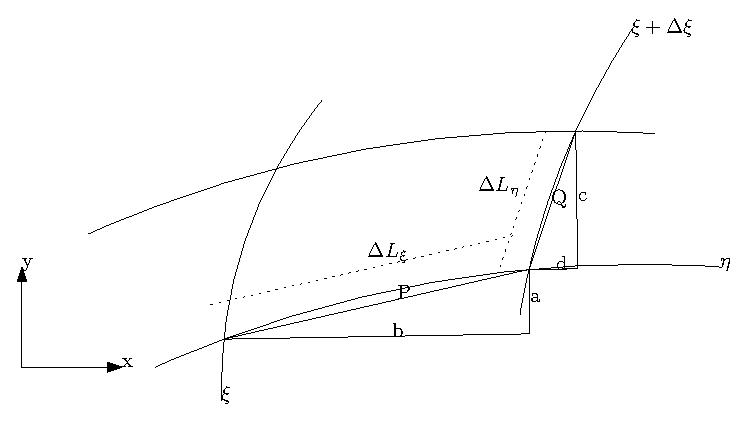
\includegraphics{fig/transformacao.eps}
    \caption{Transformação de Coordenadas}
    \label{Figura9}
\end{figure}

\begin{equation*}
    x_\xi \vert_P = \frac{x(\xi+\Delta \xi)-x(\xi)}{\Delta \xi} = \frac{b}{\Delta \xi}
\end{equation*}

Ou seja, $b=x_\xi \Delta \xi$

\begin{equation*}
    y_\xi \vert_P = \frac{y(\xi+\Delta \xi)-y(\xi)}{\Delta \xi} = \frac{a}{\Delta \xi}    
\end{equation*}

Ou seja, $a=y_\xi \Delta \xi$

\begin{equation*}
    \Delta L_\xi = \sqrt{a^2+b^2} = \sqrt{y_\xi^2 \Delta_\xi^2 + x_\xi^2+\Delta_\xi^2} = \Delta \xi \sqrt{x_\xi^2 + y_\xi^2}
\end{equation*}

Ou, escrito de outro modo:

\begin{equation}
    \label{eq:3.11}
    \Delta_\xi = \Delta \xi \sqrt{\gamma}
\end{equation}

em que:

\begin{equation}
    \label{eq:3.12}
    \gamma = x_\xi^2 + y_\xi^2
\end{equation}

\begin{equation*}
    y_\eta \vert_Q = \frac{y(\eta+\Delta \eta)-y(\eta)}{\Delta \eta} = \frac{c}{\Delta \eta}
\end{equation*}

Ou seja, $c=y_\eta \Delta_\eta$
\begin{equation*}
    x_\eta \vert_Q = \frac{x(\eta+\Delta \eta)-x(\eta)}{\Delta \eta} = \frac{d}{\Delta \eta}
\end{equation*}

Ou seja, $d=x_\eta \Delta_\eta$

\begin{equation*}
    \Delta L_\eta = \sqrt{c^2+d^2} = \sqrt{y_\eta^2 \Delta_\eta^2 + x_\eta^2+\Delta_\eta^2} = \Delta \eta \sqrt{x_\eta^2 + y_\eta^2}
\end{equation*}

Ou, escrito de outro modo:

\begin{equation}
    \label{eq:3.13}
    \Delta L_\eta = \Delta \eta \sqrt{\alpha}
\end{equation}

em que:

\begin{equation}
    \label{eq:3.14}
    \alpha = x_\eta^2 + y_\eta^2
\end{equation}

Para o cálculo da área formada por $\Delta L_\eta$ e $\Delta L_\xi$ temos, conforme a Figura \ref{fig:area}.

\begin{figure}[]
    \centering
    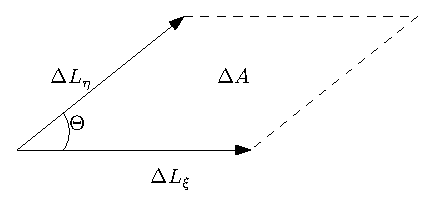
\includegraphics{fig/area.eps}
    \caption{Área}
    \label{fig:area}
\end{figure}

\begin{equation*}
    \Delta \vec{A} =
    \begin{vmatrix}
        \hat{i} & \hat{j} & \hat{k}\\
        x_\xi \Delta \xi & y_\xi \Delta \xi & 0\\
        x_\eta \Delta \eta & y_\eta \Delta -\eta & 0
    \end{vmatrix}
    = (x_\xi \Delta \xi y_\eta \Delta \eta - x_\eta \Delta \eta y_\xi \Delta \xi)\hat{k}
\end{equation*}

Assim:

\begin{equation*}
    \Delta A = x_\xi y_\eta \Delta \xi \Delta \eta - x_\eta y_\xi \Delta \xi \Delta \eta
\end{equation*}
\begin{equation*}
    \Delta A = (x_\xi y_\eta - x_\eta y_\xi)\Delta \xi \Delta \eta = J^{-1} \Delta \xi \Delta \eta\\
\end{equation*}    
\begin{equation}
    \label{eq:3.15}
    \Delta A = \frac{\Delta \xi \Delta \eta}{J}
\end{equation}

No caso tridimensional, pode-se provar que o volume físico $(\Delta v)$ é dado por:
\begin{equation}
    \label{eq:3.16}
    \Delta v = \frac{\Delta \xi \Delta \eta \Delta \gamma}{J}
\end{equation}

Sendo o jacobiano dado por:

\begin{equation}
    \label{eq:3.17}
    J = [x_\xi(y_\eta z_\gamma - y_\gamma z_\eta) - x_\eta(y_xi z_\gamma - y_\gamma z_\xi) + x_\gamma(y_\xi z_\eta - y_\eta z_\xi)]^{-1}
\end{equation}

\section{Tensor métrico 2D}

O Tensor métrico 2D é definido como:

\begin{equation}
    \label{eq:3.18}
    [g_{ij}] =
    \begin{vmatrix}
        g_{11} & g_{12}\\
        g_{21} & g_{22}
    \end{vmatrix}
    =
    \begin{vmatrix}
        \gamma & \beta\\
        \beta & \alpha
    \end{vmatrix}
\end{equation}

Em que:

\begin{equation}
    \label{eq:3.19}
    \beta = x_\xi x_\eta + y_\xi y_\eta
\end{equation}

Pode-se mostrar que o determinante do tensor métrico $g$ é dado por:

\begin{equation}
    \label{eq:3.20}
    g = \frac{1}{J^2}
\end{equation}

Das equações \ref{eq:3.20} e \ref{eq:3.18}, tem-se que:

\begin{equation*}
    \alpha \gamma - \beta^2 = \frac{1}{J^2}
\end{equation*}

E da equação \ref{eq:3.15}:

\begin{equation*}
    J=\frac{\Delta \xi \Delta \eta}{\Delta A}
\end{equation*}


Nesse caso,

\begin{equation*}
    \alpha \gamma - \beta^2 = \frac{\Delta A^2}{\Delta \xi^2 \Delta \eta^2}
\end{equation*}

Logo:

\begin{equation*}
    \Delta A^2 = (\alpha \gamma - \beta^2)\Delta \xi^2 \Delta \eta^2
\end{equation*}

Contudo,

\begin{equation*}
    \Delta A = \Delta L_\xi \Delta L_\eta \sin{\Theta} = \Delta \xi \sqrt{\gamma} \Delta \eta \sqrt{\alpha} \sin{\Theta}
\end{equation*}

Então:
\begin{equation*}
    \Delta A^2 = \Delta \xi^2 \gamma \Delta \eta^2 \alpha \sin{\Theta}^2
\end{equation*}

Igualando-se as expressões para $\Delta A^2$:
\begin{equation*}
    (\alpha \gamma - \beta^2)\Delta\xi^2 \Delta \eta^2 = \Delta \xi^2 \gamma \Delta \eta^2 \alpha \sin{\Theta}^2
\end{equation*}
\begin{equation*}
    \alpha \gamma - \beta^2 = \alpha \gamma \sin{\Theta}^2
\end{equation*}
\begin{equation*}
    \alpha \gamma(1-\sin{\Theta}^2) = \beta^2
\end{equation*}
\begin{equation*}
    \alpha \gamma \cos{\Theta}^2 = \beta^2
\end{equation*}

Ou seja:
\begin{equation}
    \label{eq:3.21}
    \beta = \sqrt{\alpha \gamma}\cos{\Theta}
\end{equation}

No caso de sistema ortogonais, $\Theta = \pi/2 = 90º$ e, portanto, $\beta = 0$. Deste modo, $\beta$ representa a não-ortogonalidade do sistema de coordenadas curvilíneas. O valor de $\Theta$ pode ser obtido para qualquer volume de controle ou malha, uma vez que ele é função de $\alpha, \beta$ e $\gamma$ que são funções das métricas.

\section{Vetores de base covariantes}
São os vetores tangentes às linhas de $\xi$ e $\eta$.

Conforme a Figura \ref{fig:e_xi} tem-se que:

\begin{equation}
    \label{eq:3.22}
    \vec{r} = x \hat{i} + y \hat{j}
\end{equation}

\begin{figure}[h]
    \centering
    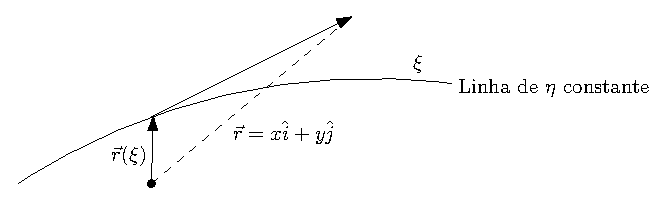
\includegraphics{fig/e_xi.eps}
    \caption{Definição de $e_\xi$}
    \label{fig:e_xi}
\end{figure}

\begin{equation}
    \label{eq:3.23}
    \vec{e_\xi} = \lim_{\Delta \xi \to 0} \frac{\vec{r}(\xi + \Delta \xi) - \vec{r}(\xi)}{\Delta \xi} = \frac{\partial \vec{r}}{\partial \xi}
\end{equation}

Portanto,

\begin{equation}
    \label{eq:3.24}
    \vec{e_\xi} = x_\xi \hat{i} + y_\xi \hat{j}
\end{equation}

que é tangente à linha de $\eta$ constante e analogamente:

\begin{equation}
    \label{eq:3.25}
    \vec{e_\eta} = x_\eta \hat{i} + y_\eta \hat{j}
\end{equation}

que é tangente à linha de $\xi$ constante.

Nota-se que, como $\hat{i}$ e $\hat{j}$ são unitários, $\vec{e_\xi}$ e $\vec{e_\eta}$ não o são.

\begin{equation}
    \label{eq:3.26}
    \vec{e_\xi} \cdot \vec{e_\xi} = x_\xi^2 + y_\xi^2 = \gamma
\end{equation}

\begin{equation}
    \label{eq:3.27}
    \vec{e_\eta} \cdot \vec{e_\eta} = x_\eta^2 + y_\eta^2 = \alpha
\end{equation}

\begin{equation}
    \label{eq:3.28}
    \vec{e_\xi} \cdot \vec{e_\eta} = x_\xi x_\eta + y_\xi y_\eta = \beta
\end{equation}

Como já mensionado, se $\beta = 0$, o sistema é ortogonal.

% PARTE DOS RESULTADOS
% ----------------------------------------------------------
\part{Resultados}
\chapter[RESULTADOS]{RESULTADOS}

\section{Malha em formato 'L'}
Conforme já especificado, a malha a ser resolvida para o problema de difusão de calor 2D é uma malha em formato 'L'. Tal malha, gerada por uma triangulação de Delaunay em um domínio fechado é apresentada na figura \ref{fig:malha-inicial}.

Nessa malha aparecem em todos as células o valor da solução analítica seguido do valor numérico encontrado. Em vermelho estão os centroides dos volumes 'Reais' e em azul o centroide dos volumes 'Virtuais'

Além de visualizar a malha, é muito útil a informação de maior ângulo, menor ângulo, desvio padrão do ângulo, média da qualidade da malha, maior qualidade, menor qualidade resultando nas tabelas \ref{tab:angulos-malha-inicial} e \ref{tab:qualidades-malha-inicial}. As qualidades se referem às qualidades de cada volume que constitui a malha, sendo que esta é obtida pela fórmula:

\begin{equation}
    2 \frac{r}{R}
    \label{eq:qualidade}
\end{equation}

Onde $r$ é o raio da circunferência inscrita e $R$ é o raio da circunferência circunscrita.
\criarsimbolo{$r$}{raio daa circunferência inscrita}
\criarsimbolo{$R$}{raio daa circunferência circunscrita}

A média das qualidades pode ser associada à malha como uma indicação da sua qualidade geral.

De modo a testar os algoritmos de suavização da malha, esta malha inicial foi distorcida, ou seja, seus vértices internos foram propositalmente alterados de posição, resultando na malha \ref{fig:malha-ruim} com as tabelas \ref{tab:angulos-malha-distorcida} e \ref{tab:qualidades-malha-distorcida}.

\newpage
\subsection{Malha Inicial}

\begin{figure}[ht]
    \centering
    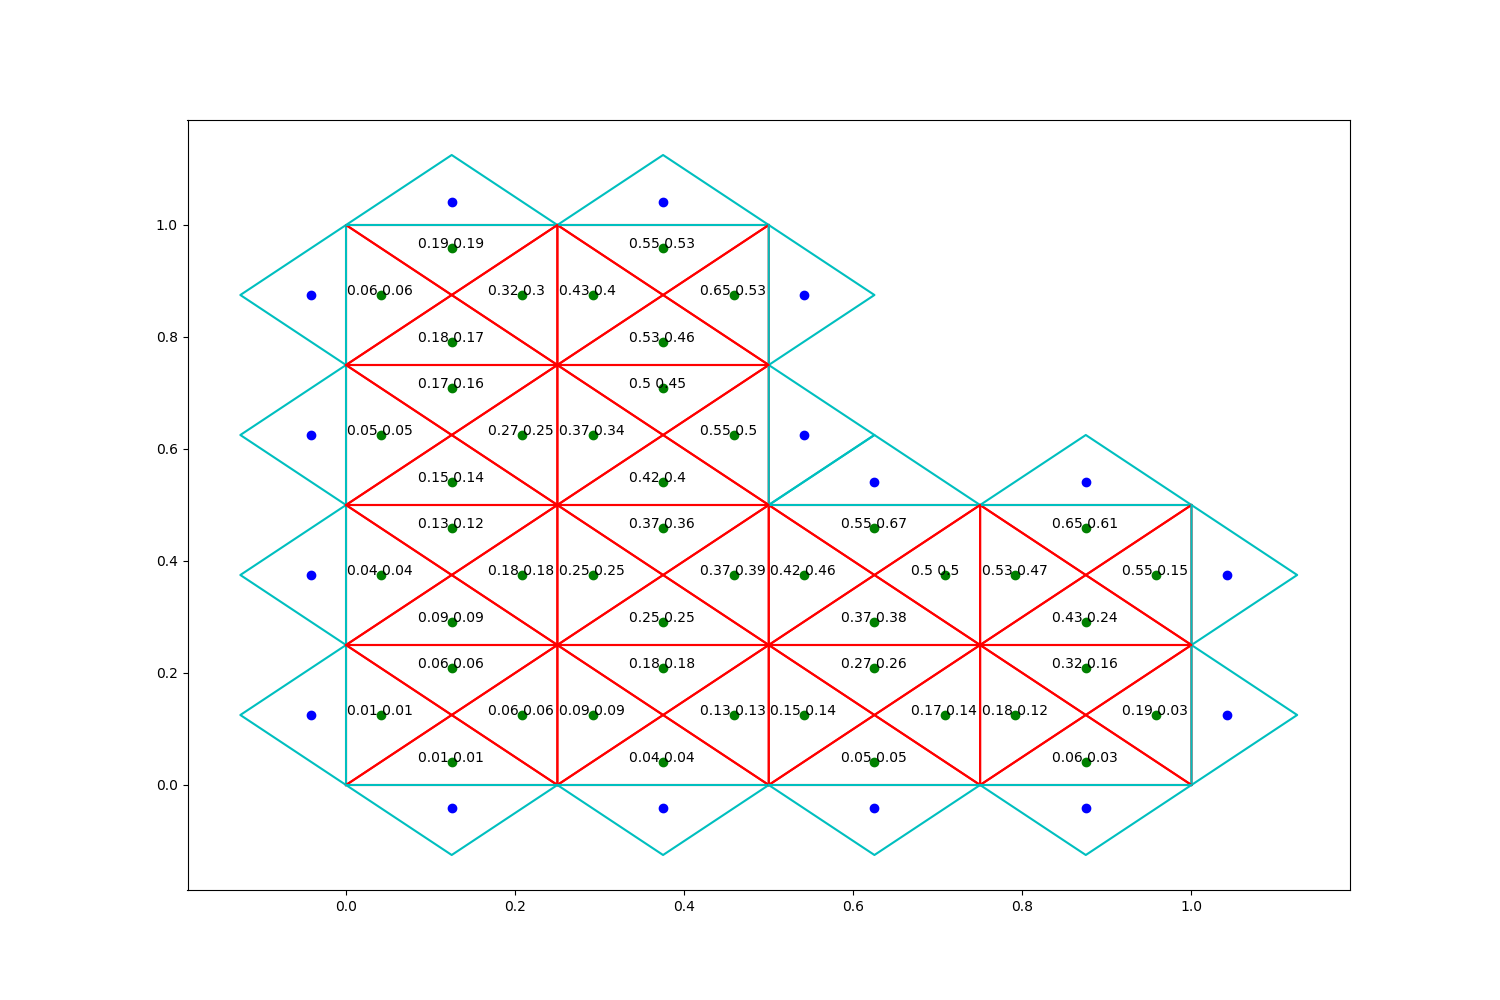
\includegraphics[width=1\linewidth]{fig/malha_inicial.png}
    \caption{Malha Inicial}
    \label{fig:malha-inicial}
\end{figure}

Na tabela \ref{tab:angulos-malha-inicial} a seguir, temos os seguintes resultados:

\begin{enumerate}
    \item Maior: Maior ângulo interno dentre todas as triangulações criadas;
    \item Menor: Menor ângulo interno dentre todas as triangulações criadas;
    \item Média: A média entre os ângulos internos de todas as triangulações, como a soma dos ângulos internos de um triângulo é sempre 180 graus, essa média é sempre 60;
    \item Desvio Padrão: O valor do desvio padrão entre os valores dos ângulos internos, quanto menor esse valor mais próximos são os valores dos ângulos e portanto mais equiláteros são os triângulos.
\end{enumerate}

\begin{table}[hb]
 \centering
 \par\caption{Ângulos da Malha Inicial}
\begin{tabular}{c|c|c|c}
 Maior&menor&média&desvio padrão\\\hline\hline
  90&45&60&21.268663\\\hline
 \end{tabular}
 \label{tab:angulos-malha-inicial}
\end{table}

Já na tabela \ref{tab:qualidades-malha-inicial} temos os seguintes resultados:

\begin{enumerate}
    \item Maior: O maior valor encontrado entre os triângulos gerados para a equação \ref{eq:qualidade};
    \item Menor: O menor valor encontrado entre os triângulos gerados para a equação \ref{eq:qualidade};
    \item Média: A média da qualidade de todos os volumes;
    \item Desvio padrão: O desvio padrão da qualidade das malhas;
\end{enumerate}

\begin{table}[h!]
 \centering
 \par\caption{Qualidades da Malha Inicial}
\begin{tabular}{c|c|c|c}
 Maior&menor&média&desvio padrão\\\hline\hline
 8.284271e-01&8.284271e-01&8.284271e-01&0\\\hline
 \end{tabular}
 \label{tab:qualidades-malha-inicial}
\end{table}

\newpage
\subsection{Malha Distorcida}

\begin{figure}[ht]
    \centering
    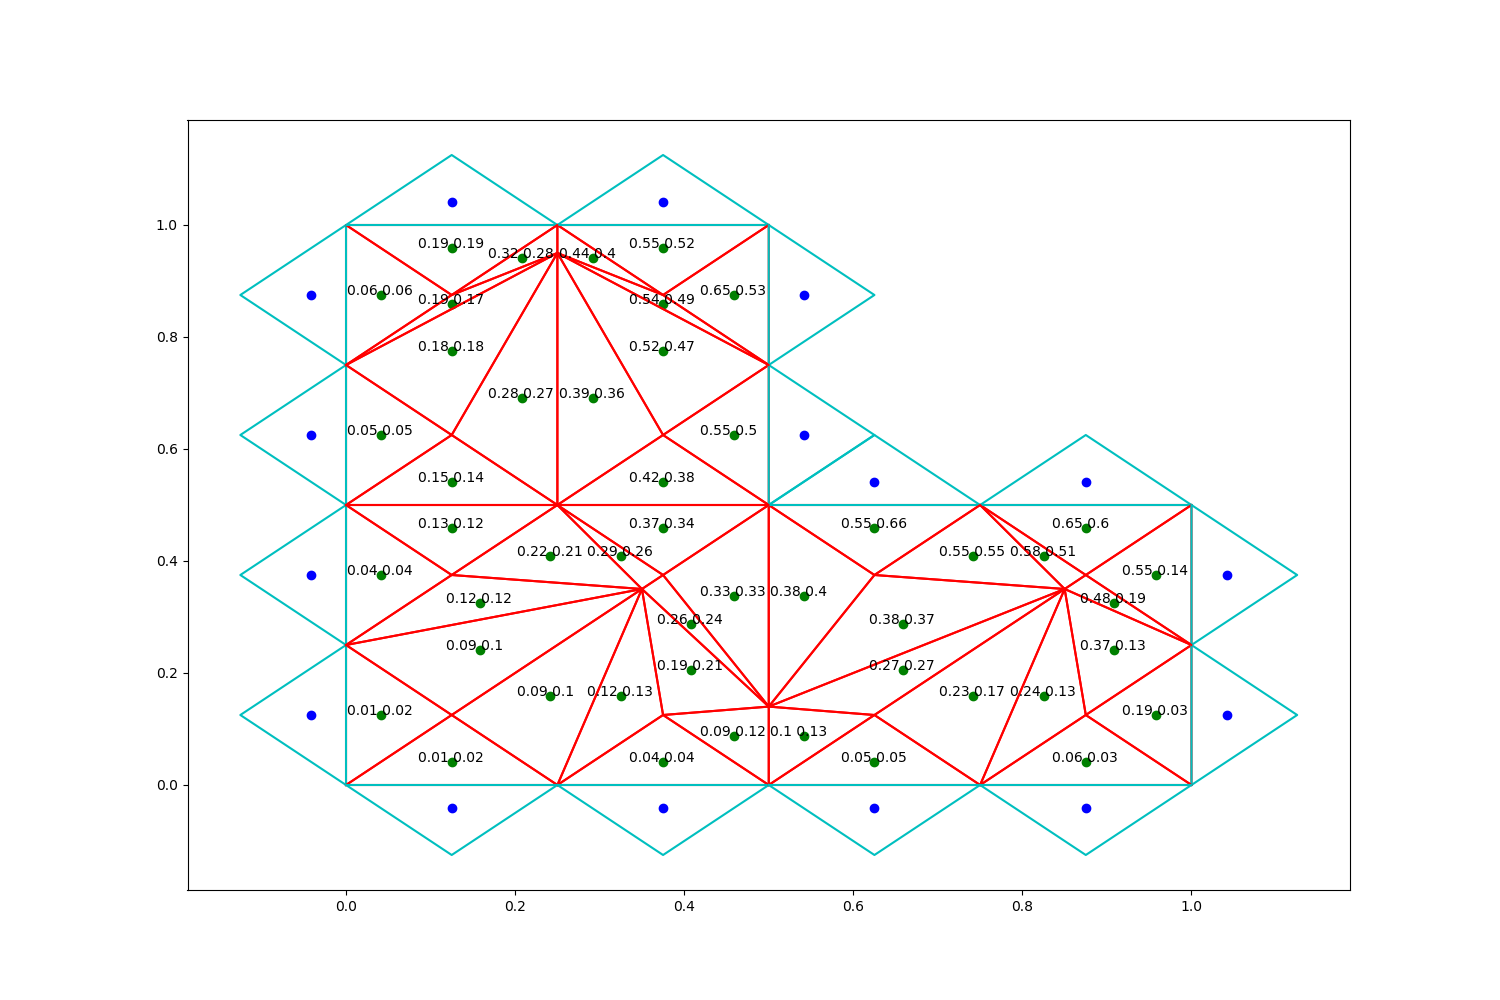
\includegraphics[width=1\linewidth]{fig/malha-ruim.png}
    \caption{Malha Inicial após Deformações}
    \label{fig:malha-ruim}
\end{figure}

Essa malha foi propositalmente distorcida de modo a se poder comparar os algoritmos de suavização. Como pode ser visto na tabela \ref{tab:angulos-malha-distorcida} o maior ângulo encontrado aumentou e o menor diminuiu. A média das qualidade de malha, que é usada como métrica da qualidade, diminuiu de valor.

\begin{table}[hb]
\centering
\par\caption{Ângulos da Malha Distorcida}
\begin{tabular}{c|c|c|c}
Maior&menor&média&desvio padrão\\\hline\hline
165.963757&6.340192&60.000000&30.017315\\\hline
\end{tabular}
\label{tab:angulos-malha-distorcida}
\end{table}



\begin{table}[hb]
\centering
\par\caption{Qualidades da Malha Distorcida}
\begin{tabular}{c|c|c|c}
Maior&menor&média&desvio padrão\\\hline\hline
0.928007&0.029467&0.700351&0.227835\\\hline
\end{tabular}
\label{tab:qualidades-malha-distorcida}
\end{table}

\newpage
\subsection{Centroidal Path Tesselation}

Em seguida, executou-se os algoritmos de melhoramento da malha com apenas uma iteração, começando pelo método centroidal patch tesselation (CPT) como na figura \ref{fig:malha-cpt}

\begin{figure}[ht]
    \centering
    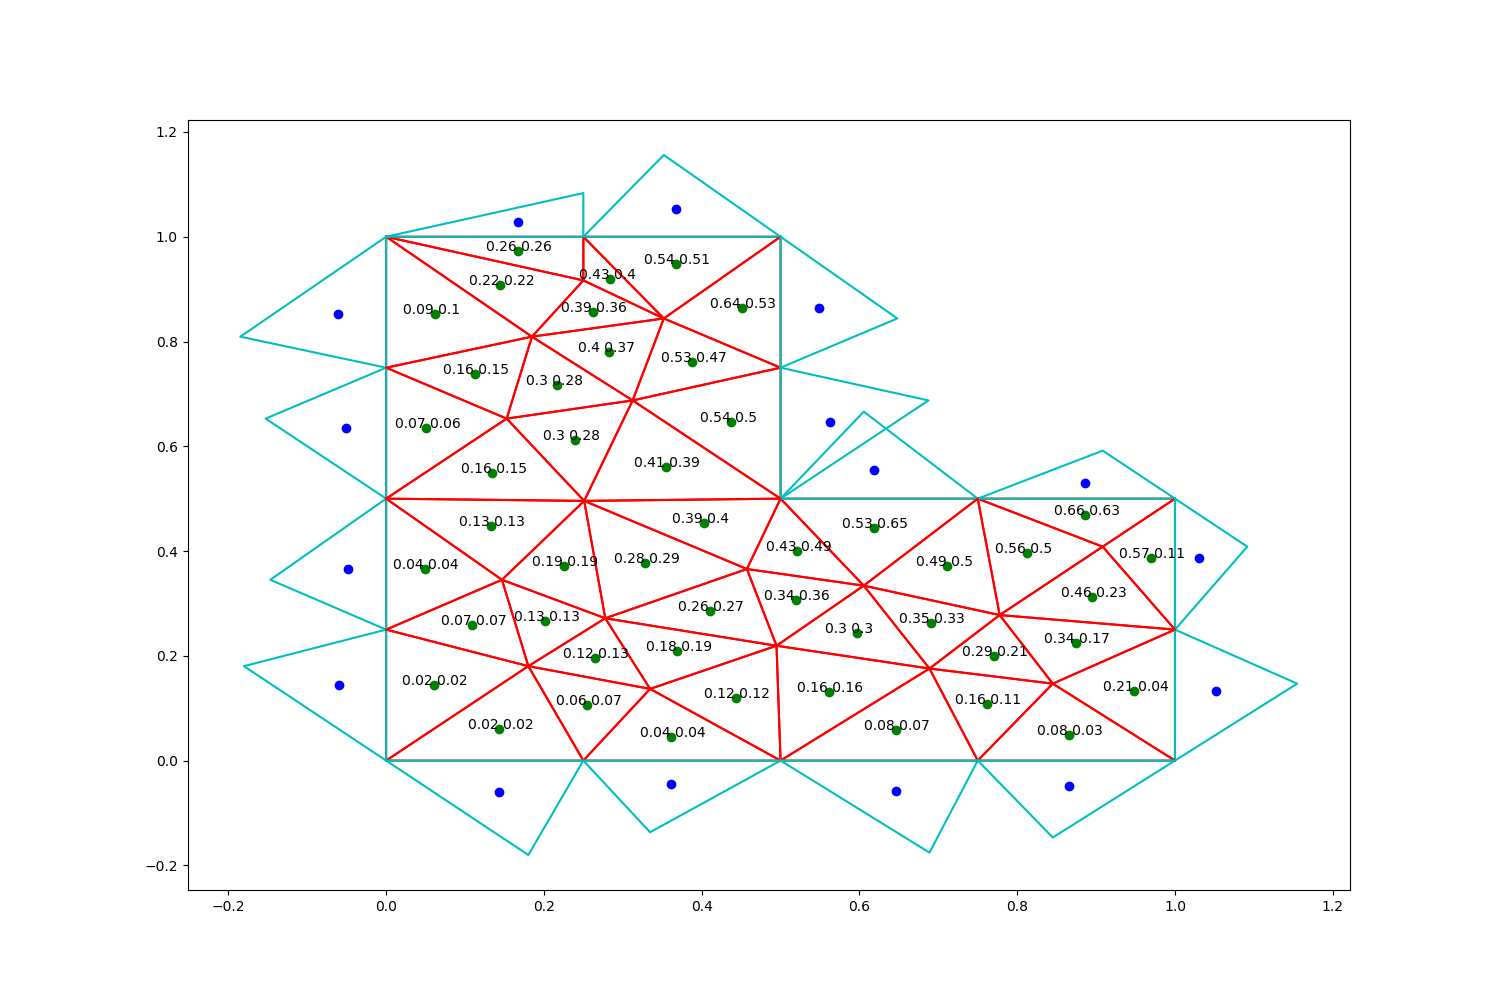
\includegraphics[width=1\linewidth]{fig/malha-cpt.png}
    \caption{Melhoramento CPT}
    \label{fig:malha-cpt}
\end{figure}

Pode-se observar que a média da qualidade aumentou de valor com essa suavização.

\begin{table}[hb]
\centering
\par\caption{Ângulos da Malha CPT}
\begin{tabular}{c|c|c|c}
Maior&menor&média&desvio padrão\\\hline\hline
125.476562&18.434949&60.000000&16.412226\\\hline
\end{tabular}
\label{tab:angulos-malha-cpt}
\end{table}

\begin{table}[hb]
\centering
\par\caption{Qualidades da Malha CPT}
\begin{tabular}{c|c|c|c}
Maior&menor&média&desvio padrão\\\hline\hline
0.997240&0.376030&0.889689&0.126673\\\hline
\end{tabular}
\label{tab:qualidades-malha-cpt}
\end{table}

\newpage
\subsection{Optimal Delaunay Tesselation}

\begin{figure}[ht]
    \centering
    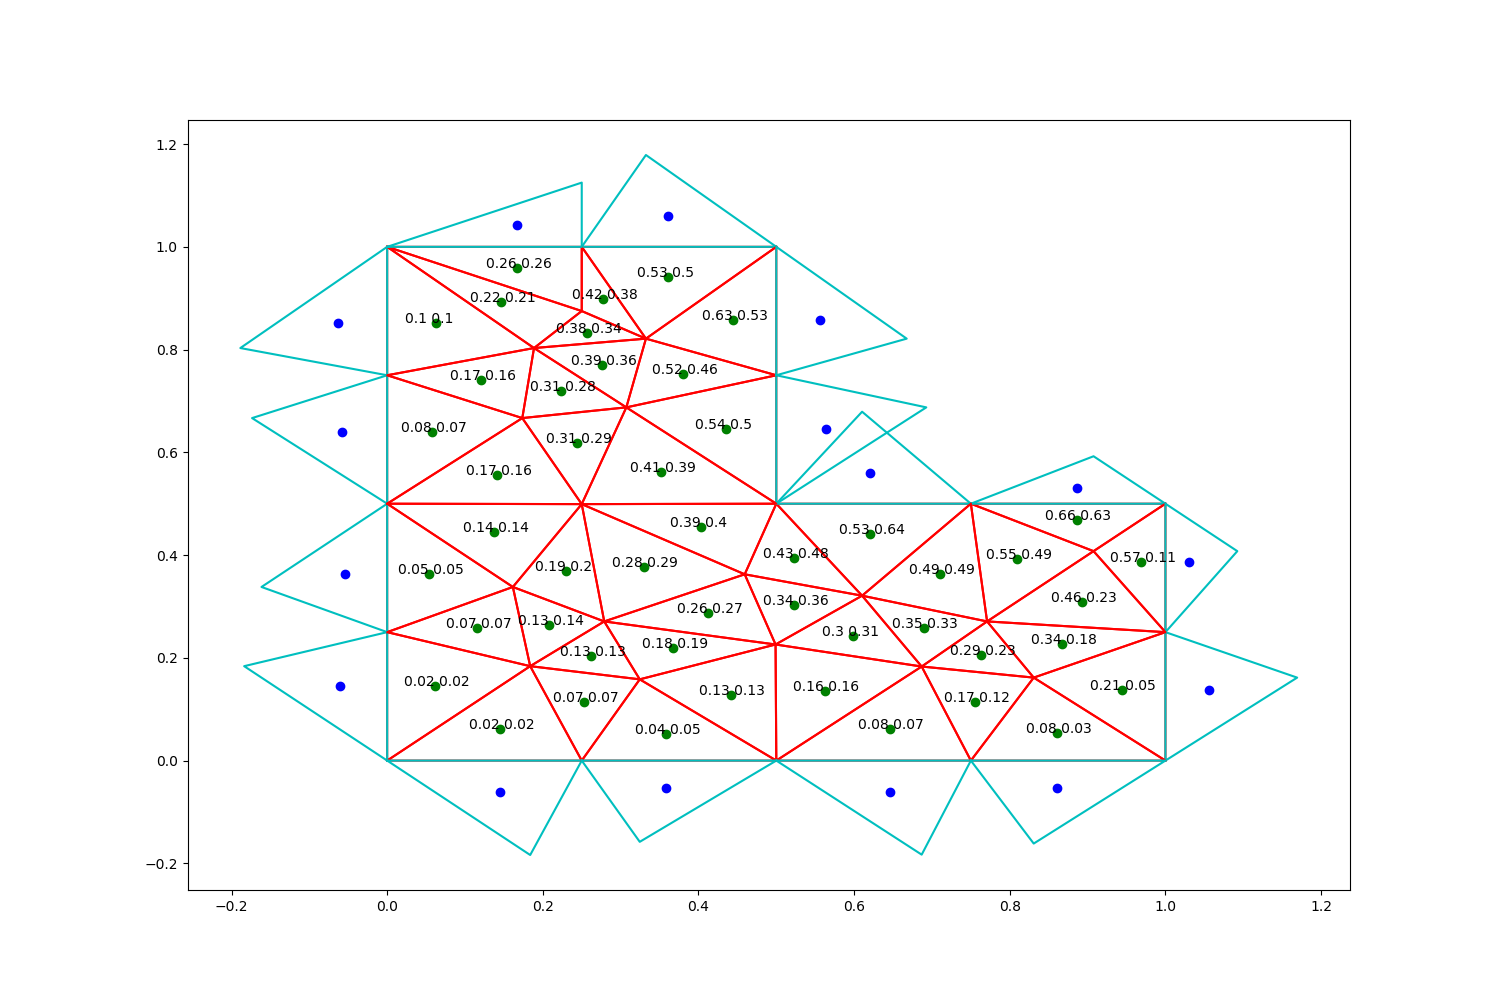
\includegraphics[width=1\linewidth]{fig/malha-odt.png}
    \caption{Melhoramento ODT}
    \label{fig:malha-odt}
\end{figure}

Esse algoritmo também apresentou um valor de média de qualidade superior em relação a malha original.

\begin{table}[hb]
\centering
\par\caption{Ângulos da Malha ODT}
\begin{tabular}{c|c|c|c}
Maior&menor&média&desvio padrão\\\hline\hline
123.086976&19.672726&60.000000&16.668335\\\hline
\end{tabular}
\label{tab:angulos-malha-odt}
\end{table}

\begin{table}[hb]
\centering
\par\caption{Qualidades da Malha ODT}
\begin{tabular}{c|c|c|c}
Maior&menor&média&desvio padrão\\\hline\hline
0.992361&0.417613&0.885554&0.119807\\\hline
\end{tabular}
\label{tab:qualidades-malha-odt}
\end{table}

\newpage
\subsection{Centroidal Voronoi Tesselation}

\begin{figure}[ht]
    \centering
    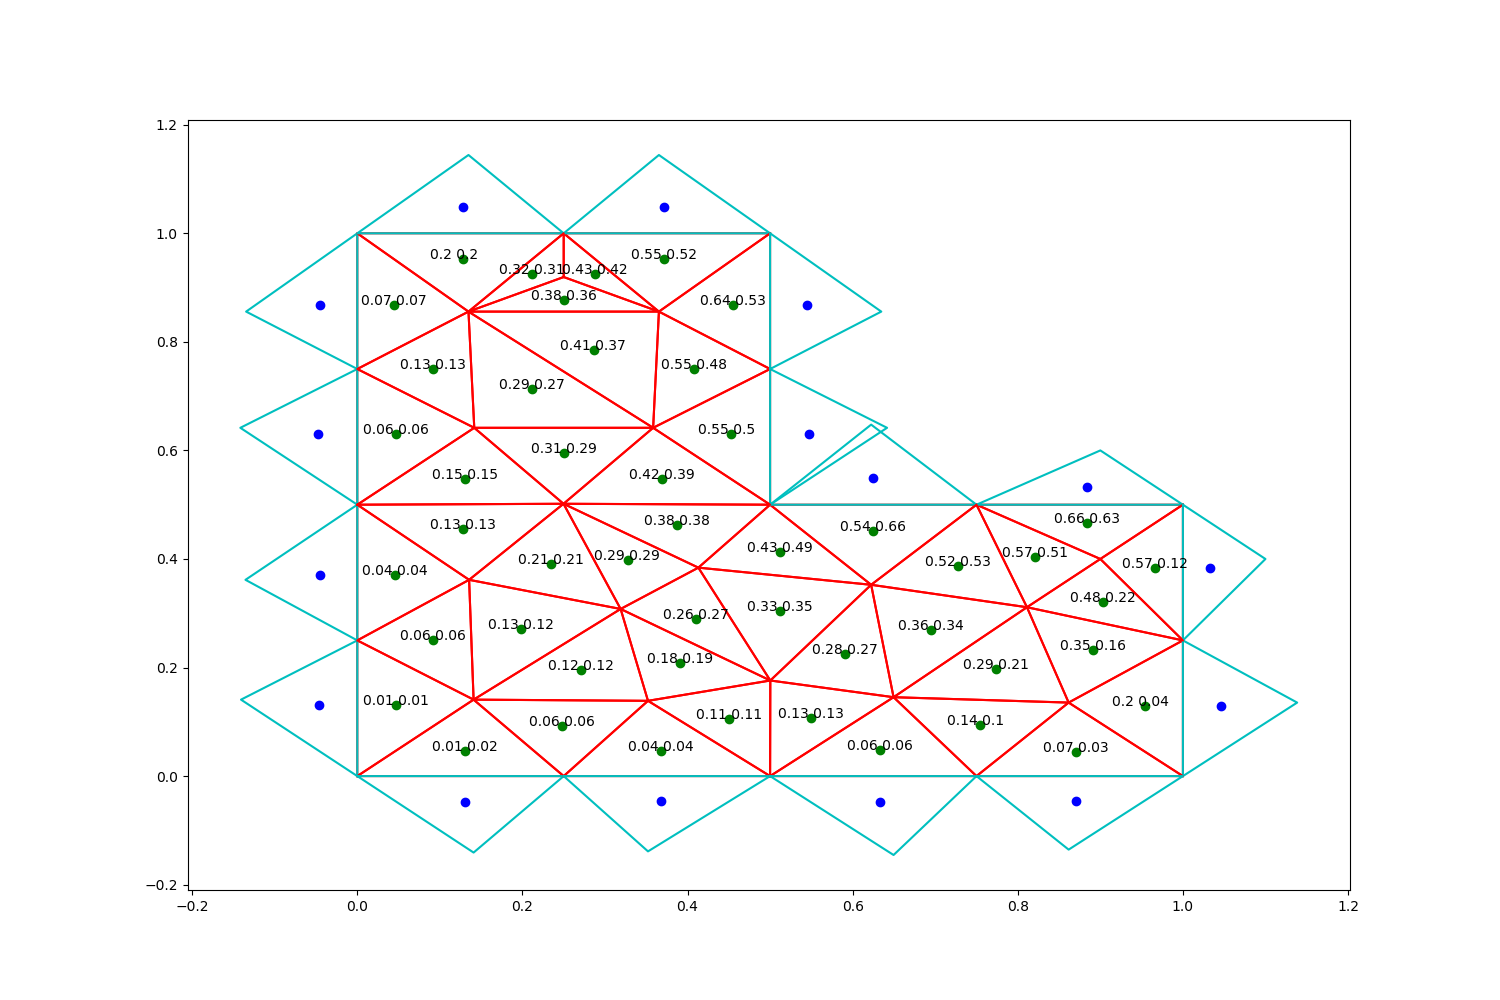
\includegraphics[width=1\linewidth]{fig/malha-cvt.png}
    \caption{Melhoramento CVT}
    \label{fig:malha-cvt}
\end{figure}

O CVT apresentou valores semelhantes aos outros algoritmos para a malha usada.

\begin{table}[hb]
\centering
\par\caption{Ângulos da Malha CVT}
\begin{tabular}{c|c|c|c}
Maior&menor&média&desvio padrão\\\hline\hline
122.171970&22.444618&60.000000&18.811931\\\hline
\end{tabular}
\label{tab:angulos-malha-cvt}
\end{table}

\begin{table}[hb]
\centering
\par\caption{Qualidades da Malha CVT}
\begin{tabular}{c|c|c|c}
Maior&menor&média&desvio padrão\\\hline\hline
0.999421&0.436461&0.865904&0.116918\\\hline
\end{tabular}
\label{tab:qualidades-malha-cvt}
\end{table}

\newpage
\subsection{Angle Based Tesselation}

\begin{figure}[ht]
    \centering
    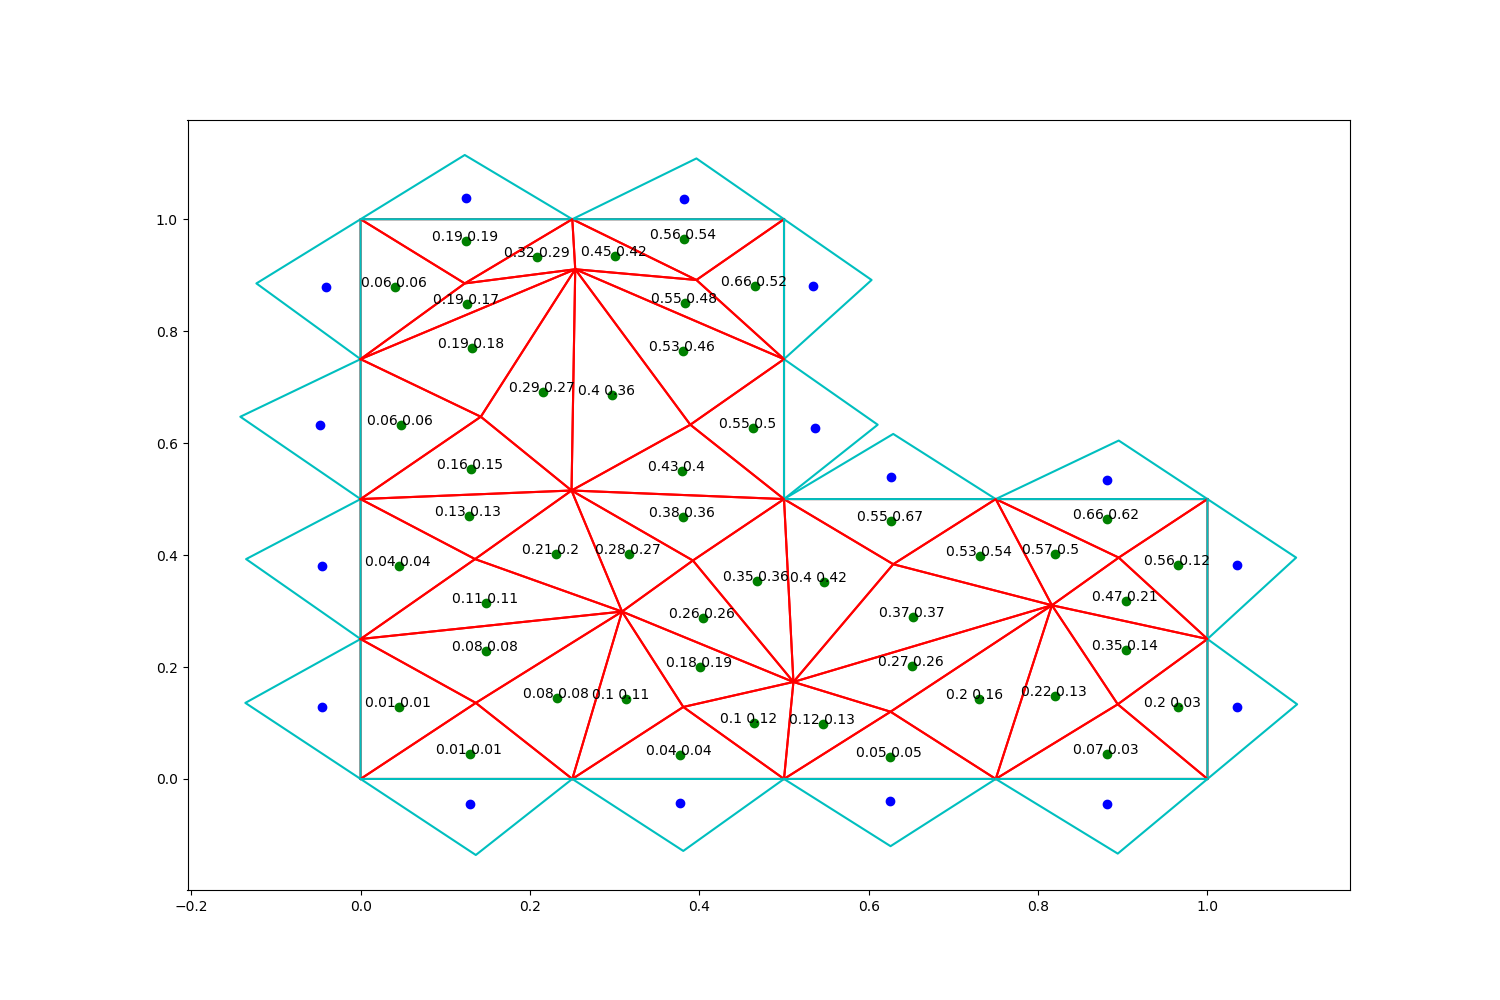
\includegraphics[width=1\linewidth]{fig/malha-angulos.png}
    \caption{Melhoramento Ângulos}
    \label{fig:malha-angulos}
\end{figure}

O algoritmo ABT resultou em uma qualidade inferior com relação aos outros métodos.

\begin{table}[hb]
\centering
\par\caption{Ângulos da Malha Ângulos}
\begin{tabular}{c|c|c|c}
Maior&menor&média&desvio padrão\\\hline\hline
143.247344&15.367140&60.000000&26.037994\\\hline
\end{tabular}
\label{tab:angulos-malha-angulos}
\end{table}

\begin{table}[hb]
\centering
\par\caption{Qualidades da Malha Ângulos}
\begin{tabular}{c|c|c|c}
Maior&menor&média&desvio padrão\\\hline\hline
0.972793&0.188339&0.758870&0.141551\\\hline
\end{tabular}
\label{tab:qualidades-malha-angulos}
\end{table}

\newpage
\subsection{Gurobi Optimization Based Tesselation}

\begin{figure}[ht]
    \centering
    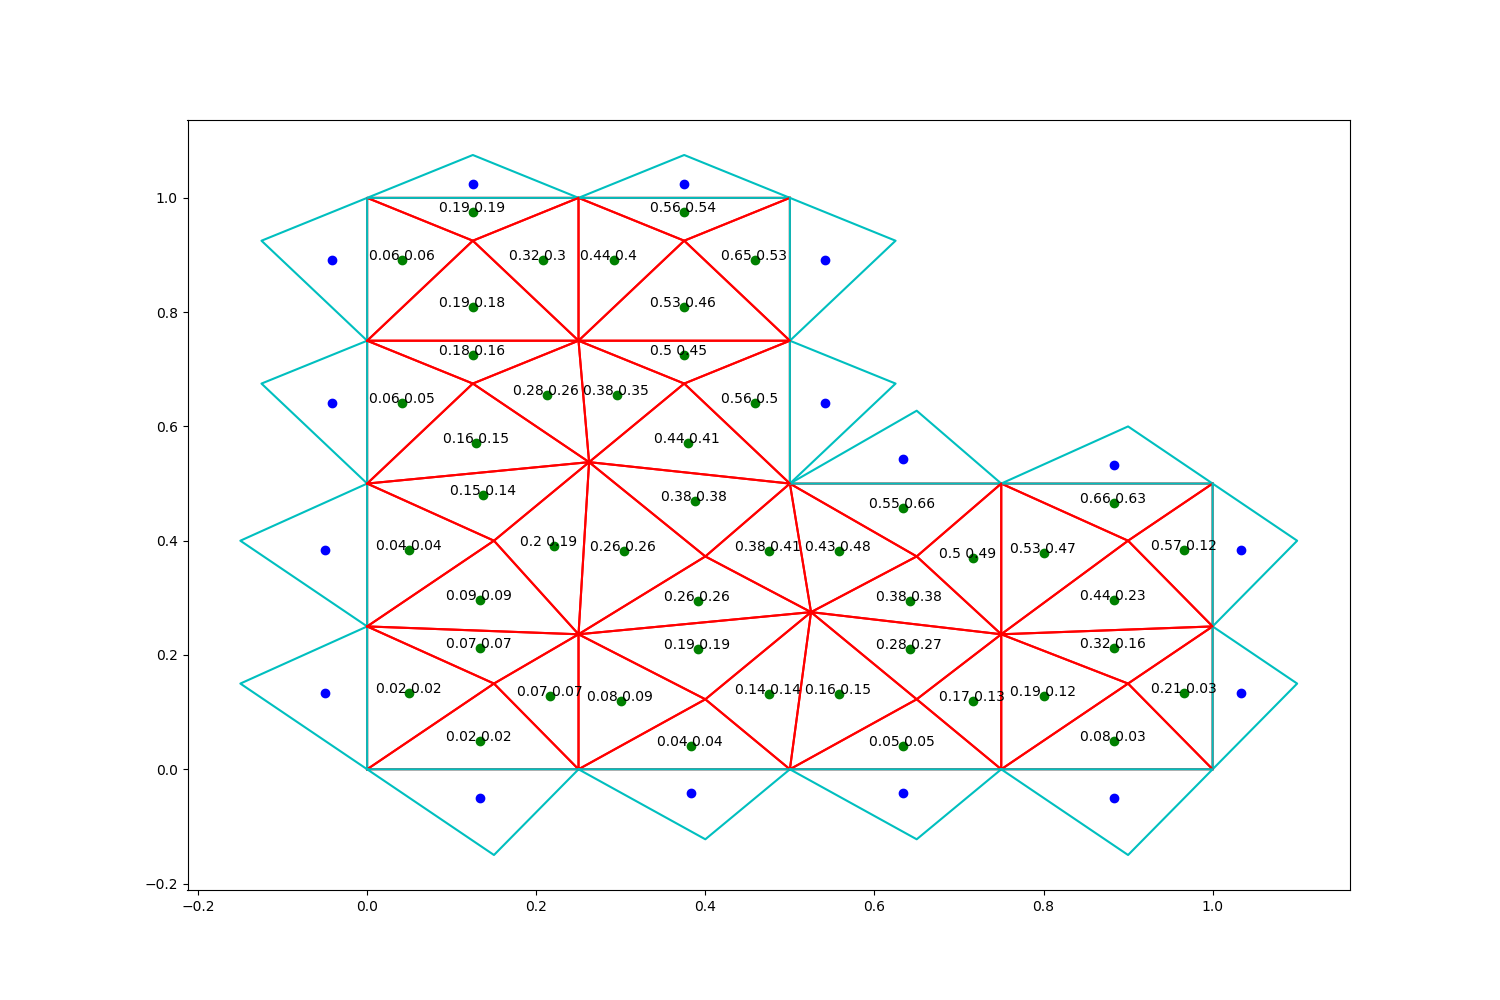
\includegraphics[width=1\linewidth]{fig/malha-gurobi.png}
    \caption{Melhoramento Gurobi}
    \label{fig:malha-gurobi}
\end{figure}

O método de suavização baseado em otimização usando-se o Gurobi resultou um valor de qualidade ligeiramente inferior, no entanto, tal resultado pode ser atribuído ao fato do modelo linear adotado usar como meta a minimização de todos os ângulos internos dos triângulos. Também deve-se levar em consideração que para uma malha maior o tempo computacional aumentaria bastante em relação aos outros métodos vistos até agora.

\begin{table}[hb]
\centering
\par\caption{Ângulos da Malha Gurobi}
\begin{tabular}{c|c|c|c}
Maior&menor&média&desvio padrão\\\hline\hline
118.072487&30.541971&60.000000&24.045397\\\hline
\end{tabular}
\label{tab:angulos-malha-gurobi}
\end{table}

\begin{table}[hb]
\centering
\par\caption{Qualidades da Malha Gurobi}
\begin{tabular}{c|c|c|c}
Maior&menor&média&desvio padrão\\\hline\hline
0.973601&0.488795&0.790714&0.134577\\\hline
\end{tabular}
\label{tab:qualidades-malha-gurobi}
\end{table}

\newpage
\subsection{Genetic Algorithm Based Tesselation}

\begin{figure}[ht]
    \centering
    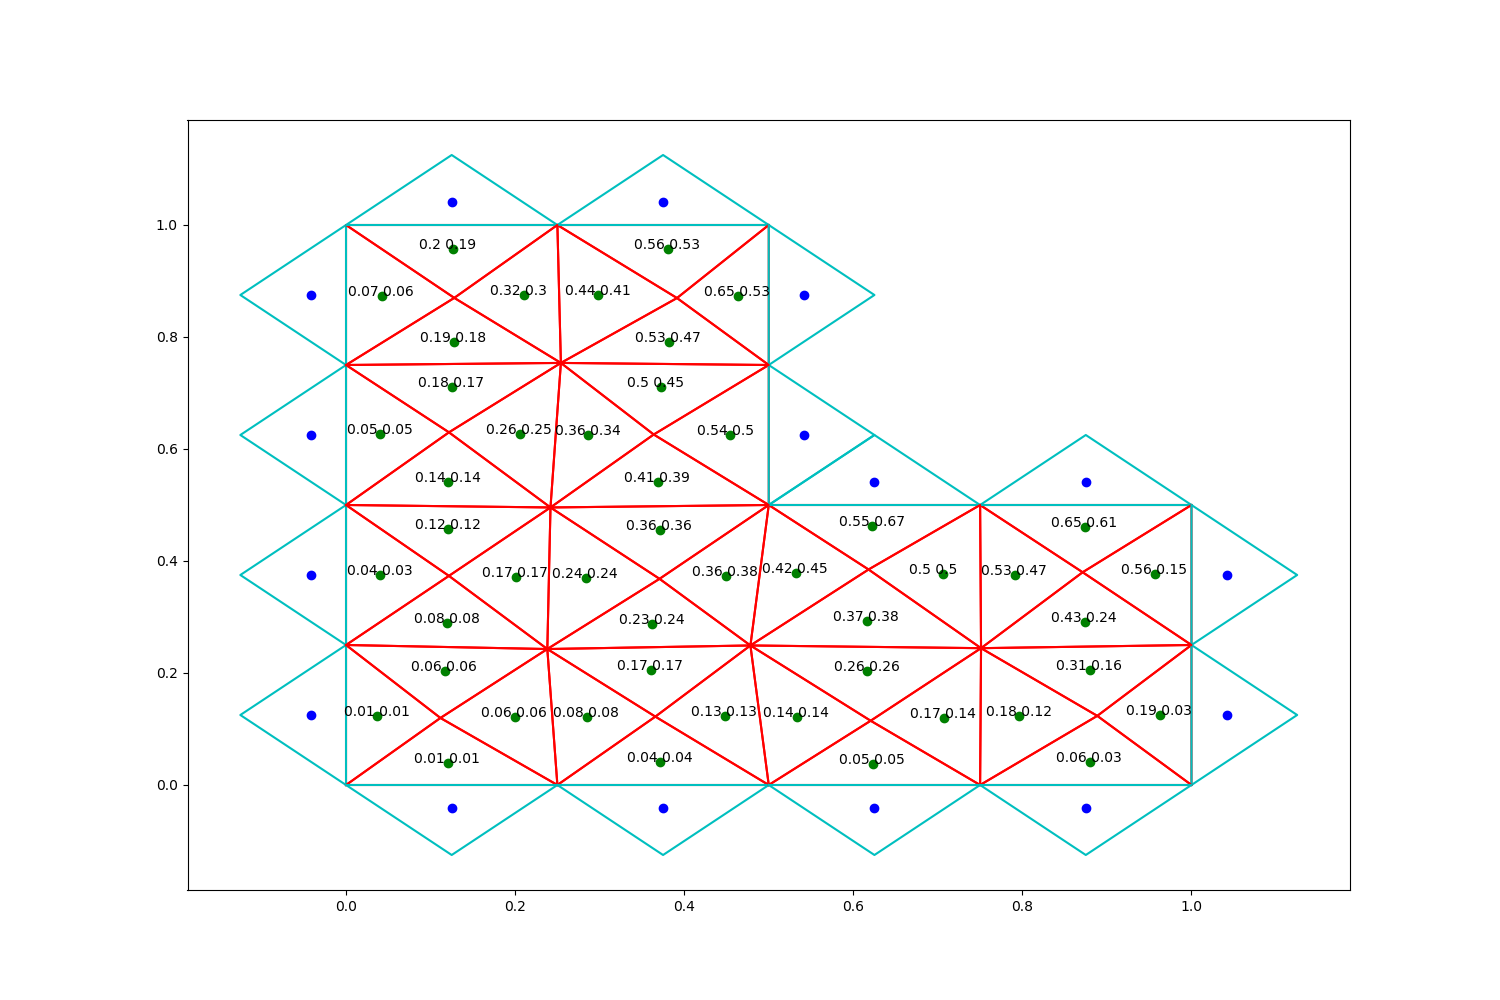
\includegraphics[width=1\linewidth]{fig/malha-ga.png}
    \caption{Melhoramento GA}
    \label{fig:malha-ga}
\end{figure}

O método de suavização baseado no algoritmo genético resultou em um bom valor para a qualidade da malha, no entanto, foi inferior aos outros métodos e teve um tempo computacional maior.

\begin{table}[hb]
\centering
\par\caption{Ângulos da Malha GA}
\begin{tabular}{c|c|c|c}
Maior&menor&média&desvio padrão\\\hline\hline
100.102771&35.502815&60.000000&21.548683\\\hline
\end{tabular}
\label{tab:angulos-malha-ga}
\end{table}

\begin{table}[hb]
\centering
\par\caption{Qualidades da Malha GA}
\begin{tabular}{c|c|c|c}
Maior&menor&média&desvio padrão\\\hline\hline
0.915087&0.715044&0.824170&0.041392\\\hline
\end{tabular}
\label{tab:qualidades-malha-ga}
\end{table}
\chapter[CONCLUSÕES]{CONCLUSÕES}

O problema proposto foi realizar uma comparação dos principais métodos de suavização de malha existentes e a criação de um novo método de suavização baseado no algoritmo genético. Para se fazer essa comparação, criou-se uma aplicação capaz de gerar uma malha triangular em formato 'L' e resolver um problema de difusão de calor com o método dos volumes finitos sendo que essa malha é do tipo não estruturada. Antes de se resolver o problema a malha passou por um outro passo do algoritmo responsável pela sua suavização, ou seja, refazer as triangulações da malha de modo a torná-las mais equiláteras e assim, diminuir os erros numéricos.

Resolveu-se o problema da suavização de malha com o algoritmo genético, esse algoritmo possui parâmetros arbitrários que são o tamanho da população, o número de gerações totais e a probabilidade de mutação. Esse algoritmo foi capaz de melhorar a malha distorcida e produziu um resultado comparável com os demais, no entanto, apresentou um tempo computacional muito maior.

De modo a ser feita a comparação entre os diferentes algoritmos de suavização, definiu-se dois tipos de métrica, o primeiro é a média das diferenças do resultado numérico em relação ao resultado analítico para todos os volumes da malha, conforme apresentado na Tabela \ref{tab:comparacao-analitico}, a segunda métrica é a média das qualidades dos volumes de controle da malha como mostrado na Tabela \ref{tab:comparacao-qualidade}.

Este trabalho abordou uma comparação entre diversos algoritmos para suavização de malhas não estruturadas e o uso do algoritmo genético como um novo processo adaptativo capaz de realizar a suavização de uma malha não estruturada. Foi apresentado o fundamento teórico que mostra a importância da geração e suavização de malhas para a solução numérica em malhas não estruturadas.

Comparando o algoritmo genético com os demais através dessas métricas tem-se que a média das diferenças em relação ao valor analítico foram muito pequenas, o que indica que em geral as soluções numéricas feitas nessa malha tiveram uma grande acurácia numérica, já a métrica da comparação entre as médias das qualidades dos volumes de controle apresentou um valor um pouco inferior aos métodos mais usados.




% Finaliza a parte no bookmark do PDF
% para que se inicie o bookmark na raiz
% e adiciona espaço de parte no Sumário
% ----------------------------------------------------------
%\phantompart

% ---
% Conclusão (outro exemplo de capítulo sem numeração e presente no sumário)
% ---
%\chapter*[Conclusão]{Conclusão}
%\addcontentsline{toc}{chapter}{Conclusão}
% ---
%\chapter[DIFUSÃO DE CALOR 2D EM REGIME PERMANENTE]{DIFUSÃO DE CALOR 2D EM REGIME PERMANENTE}

\label{dif2d}

Para o estudo da difusão de calor 2D em regime permanente, parte-se das seguintes hipóteses:
\begin{itemize}
    \item Difusão de calor 2D
    \item Regime permanente
    \item Propriedades termofísicas constantes
    \item Presença de termo fonte
\end{itemize}

Sob esses hipóteses, tem-se a seguinte equação governante:

\begin{equation}
    \label{eq:8.1}
    \frac{\partial^2 T}{\partial x^2} + \frac{\partial^2 T}{\partial y^2} = S^\phi
\end{equation}

Que pode ser reescrita como:

\begin{equation}
    \label{eq:8.2}
    \vec{\nabla} \cdot (\vec{\nabla} T) = S^\phi
\end{equation}

Tal expressão deve ser, então, integrada para cada volume de controle do domínio discretizado, de modo que:

\begin{equation}
    \label{eq:8.3}
    \int_{vc} \vec{\nabla} \cdot (\vec{\nabla}T) dv = \int_{vc}S^\phi dv
\end{equation}

Aplicando-se, na sequência, o teorema da divergência de Gauss no lado esquerdo da equação anterior, tem-se:

\begin{equation}
    \label{eq:8.4}
    \int_A \hat{n} \cdot (\vec{\nabla T}) dA = \int_{vc} S^\phi dv
\end{equation}

Ou seja,

\begin{equation}
    \label{eq:8.5}
    \sum_{superficies} \int_{\nabla A_i} \hat{n} \cdot (\vec{\Delta}T)dA = \int_{vc} S^\phi dv
\end{equation}

A integração de superfície de cada elemento é aproximada pelo produto interno entre o vetor normal (direcionado para fora do volume de controle) à superfície $\hat{n_i}$ e um vetor de fluxo difusivo $(\vec{\Delta}T)$ que atravessa a superfície do elemento de controle $(\Delta A_i)$. O primeiro termo da equação \ref{eq:8.5} pode ser aproximado empregando-se o método de diferenças centrais ao longo da linha $PA$. Deste modo,

\begin{equation}
    \label{eq:8.6}
    \int_{\Delta A_i} \hat{n_i} \cdot (\vec{\nabla}T)dA \approx \hat{n_i} \cdot (\vec{\nabla}T) \Delta A_i \approx \frac{T_A - T_P}{\Delta \xi} \Delta A_i
\end{equation}

\begin{figure}[ht]
    \begin{subfigure}{.5\textwidth}
        \centering
        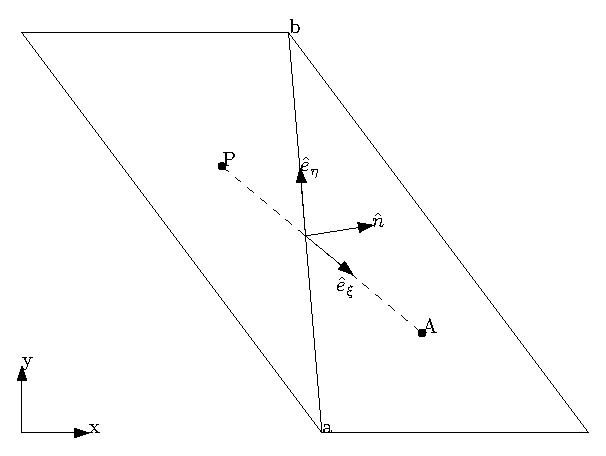
\includegraphics[width=.8\linewidth]{fig/difusao-cruzada-a.eps}
        \caption{}
        \label{fig:8.1-a}
    \end{subfigure}
    \begin{subfigure}{.5\textwidth}
        \centering
        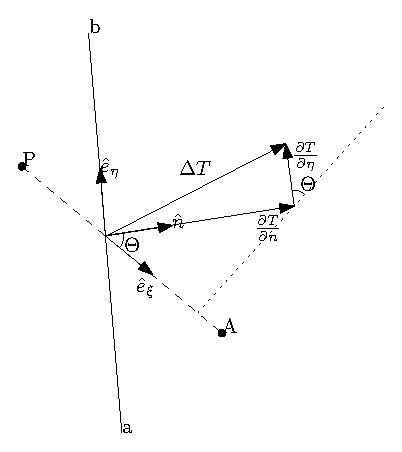
\includegraphics[width=.8\linewidth]{fig/difusao-cruzada-b.eps}
        \caption{}
        \label{fig:8.1-b}
    \end{subfigure}

    \begin{subfigure}{.5\textwidth}
        \centering
        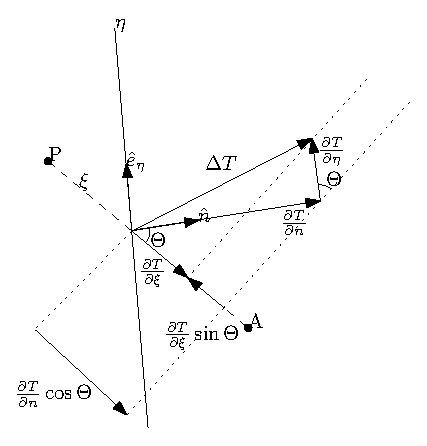
\includegraphics[width=.8\linewidth]{fig/difusao-cruzada-c.eps}
        \caption{}
        \label{fig:8.1-c}
    \end{subfigure}

    \caption{Esquemas para definição do termo de difusão cruzada}
    \label{fig:8.1}
\end{figure}

Na equação \ref{eq:8.6} $\Delta \xi$ é a distância entre os centroides A e P. Nota-se que a diferença central na equação \ref{eq:8.6} só é acurada se a linha que une os pontos A e P e o vetor normal unitário $\hat{n_i}$ estão na mesma direção, ou seja, a aproximação só é correta no caso em que a malha é completamente ortogonal. Normalmente, em malhas não-estruturadas as linhas que conectam os centroides P e A não são paralelas ao vetor normal unitário $\hat{n_i}$. Isto é conhecido como não-ortogonalidade de malha (mesh skewness ou mesh non-orthogonality). O cálculo do fluxo na equação \ref{eq:8.6} deve, desse modo, ser corrigido pela adição de uma contribuição provocada pela não-ortogonalidade. Existem diversos meios de realizar essa correção, mas a forma mais comum é a de introduzir um termo conhecido como difusão cruzada (cross diffusion), que é tratada como termo-fonte na equação discretizada.

Seguindo-se a metodologia proposta por Mathur e Murthy (1997), tem-se que o termo de difusão cruzada é obtido, introduzindo-se as coordenadas $\xi$ e $\eta$, sendo: $\xi$ definida ao longo da linha que une os pontos A e P, e $\eta$ ao longo da face do volume de controle (ao longo da linha que une os vértices a e b). Desse modo, o gradiente $\vec{\Delta}T$ pode ser expresso por:

\begin{equation}
    \label{eq:8.7}
    \vec{\nabla}T = \frac{\partial T}{\partial x}\hat{i} + \frac{\partial T}{\partial y}\hat{j} = \frac{\partial T}{\partial n}\hat{n} + \frac{\partial T}{\partial \eta}\hat{e_\eta}
\end{equation}

Sendo $\hat{i}$ e $\hat{j}$ vetores unitários nas direções $x$ e $y$ e $\hat{n}$ e $\hat{e_\eta}$ vetores unitários ao longo das direções normal e tangencial.

O vetor unitário normal $\hat{n}$, bem como os vetores unitários nas direções $\xi$ e $\eta$, $\hat{e_\xi}$ e $\hat{e_\eta}$, respectivamente, podem ser expressas através das seguintes relações envolvendo centroides e vértices:

\begin{equation}
    \label{eq:8.8}
    \hat{n} = \frac{\Delta y}{\Delta A_i}\hat{i} - \frac{\Delta x}{\Delta A_i}\hat{j} = \frac{y_b - y_a}{\Delta \eta}\hat{i} - \frac{x_b - x_a}{\Delta \eta}\hat{j}
\end{equation}

\begin{equation}
    \label{eq:8.9}
    \hat{e_\xi} = \frac{x_A - x_P}{\Delta \xi}\hat{i} + \frac{y_A - y_P}{\Delta \xi}\hat{j}
\end{equation}

\begin{equation}
    \label{eq:8.10}
    \hat{e_\eta} = \frac{x_b - x_a}{\Delta \eta}\hat{i} + \frac{y_b - y_a}{\Delta \eta}\hat{j}
\end{equation}

Uma observação que deve ser feita a respeito da equação \ref{eq:8.6} é a que ela é uma aproximação real de $\partial T/\partial \xi$ apenas no caso de uma malha ortogonal, ou seja, quando $\partial T/\partial \xi = \partial T/\partial n$. Caso contrário, para malhas não-ortogonais, $\partial T/\partial \xi$ pode ser muito diferente de $\partial T/\partial n$.

Observa-se nas figuras \ref{fig:8.1-b} e \ref{fig:8.1-c} que $\partial T/\partial \xi$ corresponde ao comprimento da projeção do vetor $\vec{\Delta}T$ na direção de $\xi$. Empregando a equação \ref{eq:8.7}, pode-se representar também $\vec{\Delta}T$ como a soma de $(\partial T/\partial n)\hat{n}$ e $(\partial T/\partial \eta)\hat{e_\eta}$, conforme a figura \ref{fig:8.1-c}.

Para se obter uma melhor estimativa do fluxo normal $\hat{n} \cdot \vec{\Delta}T = \partial T/\partial n$, examina-se a relação entre a projeção de $\vec{\Delta}T$ na direção $\xi$ que é $(\partial T/\partial \xi)$ e as projeções nessa direção de duas componentes de $\vec{\Delta}T$ que são: $(\partial T/\partial n)\hat{n} \cdot \hat{e_\xi}$ e $(\partial T/\partial \eta)\hat{e_\eta} \cdot \hat{e_\xi}$.

Denotando-se o ângulo entre as direções $\hat{n}$ e $\xi$ por $\Theta$, tem-se que:

\begin{equation}
    \label{eq:8.11}
    \frac{\partial T}{\partial n} \hat{n} \cdot \hat{e_\xi} = \frac{\partial T}{\partial n} \cos{\Theta}
\end{equation}

e

\begin{equation}
    \label{eq:8.12}
    \frac{\partial T}{\partial \eta} \hat{e_\eta} \cdot \hat{e_\xi} = - \frac{\partial T}{\partial \eta} \sin{\Theta}
\end{equation}

Deste modo, tem-se que:

\begin{equation}
    \label{eq:8.13}
    \frac{\partial T}{\partial \xi} = \frac{\partial T}{\partial n}\cos{\Theta} - \frac{\partial T}{\partial \eta} \sin{\Theta}
\end{equation}

Recorda-se, então, que $\hat{n} \cdot \vec{\Delta}T = \partial T/\partial n$ e, rearranjando os termos da equação \ref{eq:8.13}, obtém-se o fluxo difusivo da equação \ref{eq:8.6}:

\begin{equation}
    \label{eq:8.14}
    \hat{n} \cdot \vec{\Delta}T = \frac{\partial T}{\partial n} = \frac{\partial T}{\partial \xi} \frac{1}{\cos{\Theta}} + \frac{\partial T}{\partial \eta} \tan{\Theta}
\end{equation}

Os dois gradientes que transportam T no lado direito da equação \ref{eq:8.14} podem ser aproximados por diferenças centrais (CDS):

\begin{equation}
    \label{eq:8.15}
    \frac{\partial T}{\partial \xi} = \frac{T_A - T_P}{\Delta \xi}
\end{equation}

\begin{equation}
    \label{eq:8.16}
    \frac{\partial T}{\partial \eta} = \frac{T_b - T_a}{\Delta \eta}
\end{equation}

Onde $\Delta \xi$ é a distância entre os centroides $A$ e $P_i$ e $\Delta \eta$ é a distância entre os vértices $a$ e $b$ ($\Delta \eta = \Delta A_i)$.

Na literatura, tem-se que $\partial T/\partial \xi$ e $\partial T/\partial \eta$ são chamaods de gradiente direto (Direct Gradient) e difusão cruzada (Cross Diffusion), respectivamente. A substituição das aproximações por diferenças centrais, equações \ref{eq:8.15} e \ref{eq:8.16} na equação \ref{eq:8.14} resulta em:

\begin{equation}
    \label{eq:8.17}
    \hat{n} \cdot \vec{\nabla}T \Delta A_i = \frac{\Delta A_i}{\cos{\Theta}} \frac{T_A - T_P}{\Delta \xi} + \Delta A_i \tan{\Theta} \frac{T_b - T_a}{\Delta \eta}
\end{equation}

Da figura \ref{fig:8.1}, observa-se que:

\begin{equation}
    \label{eq:8.18}
    \frac{1}{\cos \Theta} = \frac{1}{\hat{n}\cdot \hat{e_\xi}} = \frac{\hat{n} \cdot \hat{n}}{\hat{n} \cdot \hat{e_\xi}}
\end{equation}

e

\begin{equation}
    \label{eq:8.19}
    \tan{\Theta} = \frac{\sin{\Theta}}{\cos{\Theta}} = - \frac{\hat{e_\xi} \cdot \hat{e_\eta}}{\hat{n} \cdot \hat{e_\xi}}
\end{equation}

Lembrando-se que:

\begin{equation}
    \label{eq:8.20}
    \vec{a} \cdot \vec{b} = |a| |b| \cos{\Theta}
\end{equation}

e

\begin{equation}
    \label{eq:8.21}
    \cos{\pi / 2 = \alpha} = - \sin{\alpha}
\end{equation}

Deste modo, a equação \ref{eq:8.17} pode ser escrita na forma vetorial como:

\begin{equation}
    \label{eq:8.22}
    \hat{n} \cdot \vec{\nabla} T \Delta A_i = \frac{\hat{n} \cdot \hat{n} \Delta A_i}{\hat{n} \cdot \hat{e_\xi}} \frac{T_A - T_P}{\Delta \xi} - \frac{\hat{e_\xi} \cdot \hat{e_\eta} \Delta A_i}{\hat{n} \cdot \hat{e_\xi}} \frac{T_b - T_a}{\Delta \eta}
\end{equation}

Os fatores $\hat{n} \cdot \hat{n} \Delta A_i / (\hat{n} \cdot \hat{e_\xi})$ e $\hat{e_\xi} \cdot \hat{e_\eta} \Delta A_i / (\hat{n} \cdot \hat{e_\xi})$ podem ser obtidos da geometria dos elementos de malha.

Normalmente, o termo de disufão cruzada é tratado como termo-fonte na equação dicretizada. Deste modo, separando-se o termo de difusão cruzada da equação \ref{eq:8.22}, obtém-se:

\begin{equation}
    \label{eq:8.23}
    \hat{n} \cdot \vec{\nabla}T \Delta A_i = \frac{\hat{n} \cdot \hat{n} \Delta A_i}{\hat{n} \cdot \hat{e_\xi}} \frac{T_A - T_P}{\Delta \xi} + S_{DC}
\end{equation}

Para a estimativa do termo de difusão cruzada, é necessário avaliar o $\vec{\nabla}T$ ao longo da linha $ab$. Existem vários métodos que podem ser empregados nesse cáclulo. Um deles consiste em interpolar os valores de $T$ nodais (obtidas para os centroides) para calcular os valores de $T_a$ e $T_b$ e então estimar o gradiente. Empregando-se a média entre todos os pontos nodais vizinhos ao vértice $a$ conduz a:

\begin{equation}
    \label{eq:8.24}
    T_a = \frac{T_P + T_A + T_B + \dots}{N}
\end{equation}

Onde $N$ é o número total de nós (centroides) ao redor do vértice $a$. Uma alternativa é empregar uma média ponderada pela distância entre o vértice e os nós, cujo resultado é mais acurado, porém, também mais caro computacionalmente.

O termo-fonte, da equação \ref{eq:8.15}, é tratado de modo semelhante ao método empregado para malhas ortogonais, ou seja:

\begin{equation}
    \label{eq:8.25}
    \int_{vc} S^\phi dv = \bar{S} \Delta v
\end{equation}

Onde $\Delta v$ é o volume do volume de controle envolvido, e $\bar{S}$ é o valor médio de $S^\phi$ sobre todo o volume de controle.

A aproximação da equação \ref{eq:8.25}, com uma aproximação de segunda ordem de acurácia, é obtida ao se empregar o teorema do valor intermediário para integrais, substituindo-se o valor médio $\bar{S}$ pelo valor nodal da função $S$ aplicado no centroide do volume de controle. No caso bidimensional, o volume $\Delta v$ corresponde à área do elemento de malha multiplicada por um comprimento unitário na direção normal ao plano bidimensional. Assim:

\begin{equation}
    \label{eq:8.26}
    \int_{vc} S^\phi dv = S_P \Delta v
\end{equation}

No caso 2D tem-se que $\Delta v = \Delta A$.

Antes de efetuar o acoplamento das diversas partes da equação discretizada para se obter o sistema de equações lineares correspondente. A equação \ref{eq:8.23} será reescrita como:

\begin{equation}
    \label{8.27}
    \hat{n} \cdot \vec{\nabla}T \Delta A_i = D_i (T_A-T_P) + S_{DC,i}
\end{equation}

Onde

\begin{equation}
    \label{eq:8.28}
    D_i = \frac{\hat{n_i} \cdot \hat{n_i}}{\hat{n_i} \cdot \hat{e_{\xi,i}}} \frac{\Delta A_i}{\Delta \xi}
\end{equation}

e

\begin{equation}
    \label{eq:8.29}
    S_{DC,i} = - \frac{\hat{e_{\xi,i}} \cdot \hat{e_{\eta,i}}}{\hat{n_i} \cdot \hat{e_{\xi,i}}} \frac{\Delta A_i}{\Delta \eta_i} (\phi_b - \phi_a)
\end{equation}

Generalizando-se a equação \ref{8.27} para todas as faces de um volume de controle e utilizando-se também a equação \ref{eq:8.26} na equação \ref{eq:8.25}, obtém-se:

\begin{equation}
    \label{eq:8.30}
    \sum_{i=1}^{nb} [ D_i (T_i - T_P) + S_{DC,i}] = S_P \Delta v
\end{equation}

No caso 2D tem-se que $\Delta v = \Delta A$ e onde:

\begin{equation}
    \label{eq:8.31}
    D_i = \frac{\hat{n_i} \cdot \hat{n_i}}{\hat{n_i} \cdot \hat{e_{\xi,i}}} \frac{\Delta A_i}{\Delta \xi}
\end{equation}

\begin{equation}
    \label{eq:8.32}
    S_{DC,i} = - \frac{\hat{e_{\xi,i}} \cdot \hat{e_{\eta,i}}}{\hat{n_i} \cdot \hat{e_{\xi,i}}} \frac{\Delta A_i}{\Delta \eta_i} (T_b - T_a)
\end{equation}

Sendo:

\begin{itemize}
    \item i: o índice referente a uma face qualquer do volume de controle
    \item nb: a quantidade total de faces do volume de controle
    \item P: o índice do centroide do volume de controle considerado
    \item Ti: a temperatura no centroide do volume de controle vizinho ao volume P, com compartilhamento da face i
    \item $\hat{n_i}$: o vetor normal unitário à face i, que aponta para fora do volume P
    \item $\hat{e_{\xi,i}}$: vetor unitário na direção $\xi$, para a face i
    \item $\hat{e_{\eta,i}}$: vetor unitário na direção $\eta$, para a face i
    \item $\xi$: direção da linha que une os centroides do volume P e do volume vizinho com compartilhamento da face i
    \item $\eta$: direção da linha que une os vértices a e b, pertencentes à face i
    \item $\Delta A_i$: área da face i, no caso 2D, $\Delta A_i = \Delta \eta$
    \item $\Delta v$: volume total do volume de controle P, no caso 2D, $\Delta v = \Delta A$ (área do elemento de malha).
    \item $T_b, T_a$: temperaturas avaliadas nos vértices $b$ e $a$, respectivamente, da face i (é conveniente que $b$ e $a$ estejam dispostos de tal modo que a ordenação dos vértices esteja no sentido anti-horário)
\end{itemize}

A equação \ref{eq:8.30} pode ser rearranjada para a forma:

\begin{equation}
    \label{eq:8.33}
    a_P T_P = \sum a_{nb} T_{nb} + b_P
\end{equation}

Sendo:

\begin{equation}
    \label{eq:8.34}
    a_P = \sum a_{nb}
\end{equation}

\begin{equation}
    \label{eq:8.35}
    \sum a_{nb} = \sum_{i=1}^{nb} S_{DC,i}
\end{equation}

\begin{equation}
    \label{eq:8.36}
    b_P = -S_P \Delta v = \sum_{i=1}^{nb} S_{DC,i}
\end{equation}

O sistema de equações, na forma da equação \ref{eq:8.33}, pode ser resolvido por qualquer método para solução de sistemas lineares. Caso o método escolhido seja o de Gauss-Seidel, tem-se que:

\begin{equation}
    \label{eq:8.37}
    T_P = (\sum a_{nb}T_{nb}+b_P)/a_P
\end{equation}

\section{Algoritmo}

O algoritmo apresenta os seguintes passos:

\begin{enumerate}
    \item Gerar a malha: tipos de elementos, vértices, centroides, conectividades
    \item Para um volume de controle P, calcular os coeficientes $a_P$ e $\sum a_{nb}$. Para tanto, é necessário.
    \begin{enumerate}
        \item Em cada face i, definem-se os vetores unitários: normal à superfície $(\hat{n})$, na direção da linha que une os vértices $a$ e $b$ da face $(\hat{e_\eta})$, e na direção da linha que une o centroide de P e o centroide do volume que compartilha a face i $(\hat{e_\xi})$: equações \ref{eq:8.8} a \ref{eq:8.10}, no caso 2D.
        \item Obter o valor de $D_i$, referente à face i, pela equação \ref{eq:8.28}
        \item Voltar ao passo 2a, para que sejam obtidos todos os vetores unitários $(\hat{n}, \hat{e_\xi}, \hat{e_\eta})$, bem como todos os valores de $D_i$ para as $nb$ faces do volume de controle, obtendo-se então todos os coeficientes $a_{nb}$.
    \end{enumerate}
    \item Calcular o termo-fonte $b_P$. Para tanto, é necessário calcular $\Delta v$ para o volume de controle P (no caso 2D, $\Delta v = \Delta A$). É necessário, também, avaliar a função $S^\phi$ no centroide do volume P, bem como calcular $S_{DC,i}$ para todas as $nb$ faces do volume P. Para o cálculo das temperaturas nos vértices, pode-se empregar a equação \ref{eq:8.24}, utilizando-se todos os centroides cujos volumes são construídos empregando-se o vértice em questão.
    \item Retornar ao passo 2, até que todos os volumes de controle da malha sejam avaliados.
    \item Resolver o sistema linear obtido através de um método como o de Gauss-Seidel, equação \ref{eq:8.37}
    \item Recalcular os termos-fontes de todos os volumes (Passo 3).
    \item Voltar ao passo 5 até que um dado critério de parada (Tolerância, número de iterações) seja atingido.
\end{enumerate}

\section{Condições de contorno}
A aplicação das condições de contorno pode ser realizada com o auxílio, por exemplo, de volumes fictícios. Neste caso, duas possibilidades são listadas:

\subsection{Volume espelhado}

Também chamado de volume simétrico, neste caso, apesar do vetor normal à superfície de controle que separa os volumes A e P ser paralelo à linha que une A a P, nota-se que há um desalinhamento entre o ponto médio da face (m) e a linha $\bar{AP}$. Neste caso, existe um erro de discretização relacionado ao fato de a linha $\bar{PA}$ não interceptar o ponto médio $m$ da face $ab$. Esse erro cresce com o aumento da não-ortogonalidade da malha, bem como com o aumento da razão de aspecto da malha como pode ser visto na figura \ref{contorno-1}.

\begin{figure}[h]
    \centering
    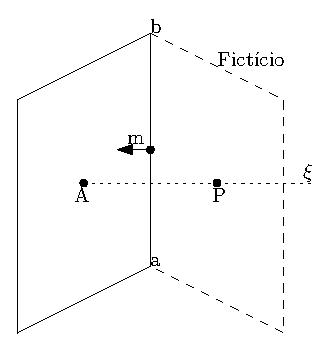
\includegraphics{fig/contorno-1.eps}
    \caption{Volume Espelhado}
    \label{contorno-1}
\end{figure}

Outro modo de se aplicar as condições de contorno com volumes fictícios é feita empregando-se um volume antissimétrico, ou seja, ele deve ser espelhado em ambas as direções (e e y), como se segue:

\subsection{Volume antissimétrico}

\begin{figure}[]
    \centering
    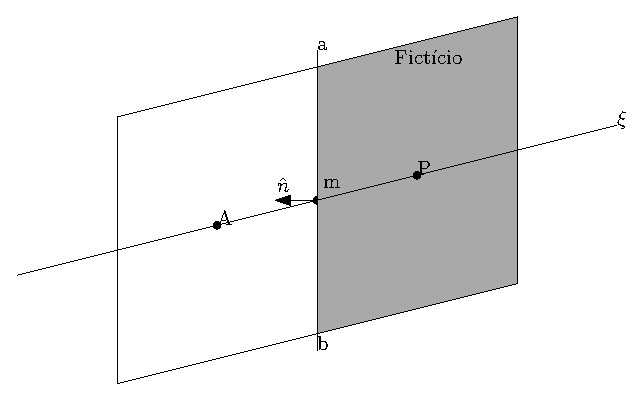
\includegraphics{fig/contorno-2.eps}
    \caption{Volume Antissimétrico}
    \label{contorno-2}
\end{figure}

Neste caso, a linha que une P e A passa pelo ponto médio da face $(m)$. Assim, não há o erro de não-ortogonalidade existente ao se aplicar o volume fictício espelhado (simétrico). Nota-se, contudo, que será necessário avaliar o termo de difusão cruzada, uma vez que o vetor normal $\hat{n}$ e o vetor unitário na direção $\xi$ podem não ser coincidentes. Nesse caso, será necessário empregar uma expressão semelhante à equação \ref{8.27}. Contudo, a temperatura nos vértices $T_a$ e $T_b$ pode ser avaliada mediante o uso das condições de contorno.

Uma importante observação a respeito da utilização de diferenças centrais envolvidas na integração da superfície dos elementos de controle diz respeito ao fato que sua acurácia será de segunda ordem apenas no caso em que as mesmas sejam avaliadas no ponto médio de $\hat{n} \cdot \vec{\nabla}T \Delta A_i$. Este não é o caso se as linhas PA e ab não se interceptam no ponto médio m de ab quando a malha é não-ortogonal.

Este erro aumenta com a não-ortogonalidade e a razão de aspecto da malha, de modo que um grande esforço deve ser feito com relação ao controle da não-ortogonalidade e da razão de aspecto em malhas não-estruturadas.


% ELEMENTOS PÓS-TEXTUAIS
% ----------------------------------------------------------
\postextual


% Referências bibliográficas
% ----------------------------------------------------------
%\bibliography{referencias}


\printbibliography[heading=bay]
% ----------------------------------------------------------


% Glossário
% ----------------------------------------------------------
% Consulte o manual da classe abntex2 para orientações sobre o glossário.
%
%\glossary

% Apêndices
% ----------------------------------------------------------
\ifthenelse{\equal{\terApendice}{Sim}}
{\begin{apendicesenv}

% Imprime uma página indicando o início dos apêndices
\partapendices

   % Existem várias formas de se colocar anexos.
   % O exemplo abaixo coloca 2 apêndices denominados de 
   % DESENVOLVIMENTO DETALHADO DA PINTURA e 
   % ESCOLHA DO MATERIAL DE IMPRESSÃO:
   % ---
   % --- insere um capítulo que é tratado como um apêndice
   %\chapter{DESENVOLVIMENTO DETALHADO DA PINTURA}
   % 
   %\lipsum[29] % gera um parágrafo
   %
   % --- insere um capítulo que é tratado como um apêndice
   %\chapter{ESCOLHA DO MATERIAL DE IMPRESSÃO}
   % 
   %\lipsum[30] % gera um parágrafo


% --- Insere o texto do arquivo ap01.tex
% 
% --- O conteúdo do arquivo pode ser vários anexos ou um único apêndices.
%     A vantagem de se utilizar este procedimento é de suprimi-lo
%     das compilações enquanto se processa o resto do documento.

\input{ap01}

\end{apendicesenv}
}{}


% Anexos
% ----------------------------------------------------------
\ifthenelse{\equal{\terAnexo}{Sim}}{
\begin{anexosenv}

% --- Imprime uma página indicando o início dos anexos
 \partanexos

   % Existem várias formas de se colocar anexos.
   % O exemplo abaixo coloca 2 anexos denominados de 
   % TABELA DE VALORES e GRÁFICOS DE BALANCEMANTO:
   % ---
   % --- insere um capítulo que é tratado como um anexo
   %\chapter{TABELAS DE VALORES}
   % 
   %\lipsum[31] % gera um parágrafo
   %
   % --- insere um capítulo que é tratado como um anexo
   %\chapter{GRÁFICOS DE BALANCEAMENTO}
   % 
   %\lipsum[32] % gera um parágrafo


% --- Insere o texto do arquivo ax01.tex
% 
% --- O conteúdo do arquivo pode ser vários anexos ou um único anexo.
%     A vantagem de se utilizar este procedimento é de suprimi-lo
%     das compilações enquanto se processa o resto do documento.

 \input{ax01} 


\end{anexosenv}
}{}

% INDICE REMISSIVO
%---------------------------------------------------------------------
\ifthenelse{\equal{\terIndiceR}{Sim}}{
\phantompart
\printindex
}{}

\end{document}
